\chapter{Переход между искажёнными ориентационными структурами в случае большого усреднённого флексоэлектрического коэффициента.}\label{ch:ch5}
В предыдущей главе рассматривалась ситуация, когда при достаточно больших значениях $\bar{e}$ и $U$ выполнялось соотношение
\begin{equation}\label{criterion_eU}
\frac{\bar{e}U}{K}\gg 1,
\end{equation}
где $K = \max{K_{ii}}$ -- наибольший модуль Франка рассматриваемой системы.
При этом вкладами в свободную энергию $\FF_\mathrm{tot}$, даваемую выражением~\eqref{eq:free-energy}, содержащими $K_{ii}$ и $ W_\phi^{(1,2)}$, можно пренебречь.
Таким образом, выражение для свободной энергии может быть записано в следующем виде:
\begin{multline}\label{eq_F_f_final1_ch5}
\FF = \frac{S_\bot}{2} \bigg(-\frac{1}{4\pi}U^2 J + 2 \bar{e}U JJ_1 + 4\pi \bar{e}^2\int_{0}^{L}\frac{(\sin 2\theta \,\theta'-JJ_1)^2}{{\EE}(\theta)}dz +\\
+ W_\theta^{(1)} {\sin^2\big( \theta(0) - \theta_0^{(1)}\big)} + W_\theta^{(2)} {\sin^2\big( \theta(L) - \theta_0^{(2)}\big)}\bigg).
\end{multline}
Видно, что в этом пределе свободная энергия не зависит от азимутального угла $\phi(z)$, а значит, в этом случае нематические и холестерические ЖК описываются одинаково.

Исследуем, как равновесная ориентационная структура ЖК-ячейки (описываемая зависимостью $\theta(z)$) меняется в зависимости от приложенного напряжения $U$ для различных наборов материальных параметров.
В дальнейшем ограничимся углами лёгкого ориентирования на границах $\theta_0^{(1,2)} = \pi/2$.
Отметим, что в этом приближении свободная энергия~\eqref{eq_F_f_final1_ch5} является функционалом $\cos^2\theta(z)$.
Таким образом, удобно использовать замену $y(z)\equiv \cos^2\theta(z) + \ve_\bot/\ve_a = \EE(\theta)/\ve_a$.
Так как ранее мы указывали, что ищем функцию $\theta(z)\in C^2[0,\, L]$, то и на $y(z)$ накладываются такие же требования: $y(z)\in C^2[0,\, L]$. 
При этом важно, что функция $y(z)$ ограничена: $y(z)\in \left[{\ve_\bot}/{\ve_a},\ {\ve_\| }/{\ve_a}\right]\ \forall z\in[0,L]$.
Свободная энергия как функционал $y(z)$ имеет вид
\begin{multline}\label{eq_F_f_final_y}
\FF = \frac{S_\bot}{2}\bigg(-\frac{1}{4\pi}U^2 J + 2 \bar{e}U JJ_1 + \frac{4\pi \bar{e}^2}{\ve_a}\int_{0}^{L}\frac{(y'+JJ_1)^2}{y}dz +\\
+ W_\theta^{(1)}y(0) + W_\theta^{(2)}y(L) - (W_\theta^{(1)} + W_\theta^{(2)})\frac{\ve_\bot}{\ve_a}\bigg).
\end{multline}
В терминах $y(z)$ можно также записать
\begin{equation}\label{D_z=UJ_y}
J^{-1}= \ve_a^{-1}\int_0^L \frac{dz}{y},\quad J_1=\varepsilon_a^{-1}\ln\frac{y(0)}{y(L)}.
\end{equation}
Для того, чтобы рассчитать равновесную ориентационную конфигурацию $\theta(z)$, нужно найти функцию $y(z)$, доставляющую минимум функционалу~\eqref{eq_F_f_final_y}.
Так как функция $y(z)$ ограничена, необходимое условие минимизации свободной энергии можно сформулировать как неотрицательность её первой вариации
\begin{equation}
\delta \FF \geq 0.
\label{eq:dF1}
\end{equation}
Вариация $\delta\FF$ даётся следующей формулой:
\begin{equation}\label{eq:dF_ch5}
\begin{aligned}
\frac{\delta\FF}{S_\bot} = 
&\left[ \frac{-U^2 J^2}{8\pi} + \bar{e}U J_1 J^2 + 2\pi\bar{e}^2 \left( (y')^2 - 2y''y - J_1^2 J^2 \right) \right] \frac{\delta y(z)}{\ve_a y^2} + \\
&+\left[ \bar{e}UJ - 4\pi\bar{e}^2\left( y'(0) + JJ_1 \right) + \ve_a y(0) \frac{W_1}{2} \right] \frac{\delta y(0)}{\ve_a y(0)} + \\
&+\left[ -\bar{e}UJ + 4\pi\bar{e}^2\left( y'(L) + JJ_1 \right) + \ve_a y(L) \frac{W_2}{2} \right] \frac{\delta y(L)}{\ve_a y(L)}.
\end{aligned}
\end{equation}
При этом функция $y(z)$ должна удовлетворять условиям
\begin{subequations}
	\begin{empheq}[left = \empheqlbrace]{align}
		&0\leq z \leq L,\label{eq:rectangle_1}\\
		&\ve_\bot/\ve_a \leq y \leq \ve_\| /\ve_a.\label{eq:rectangle_2}
	\end{empheq}
\end{subequations}
\begin{figure}\label{pic:Allowed_areas_for_y}
	\centering
	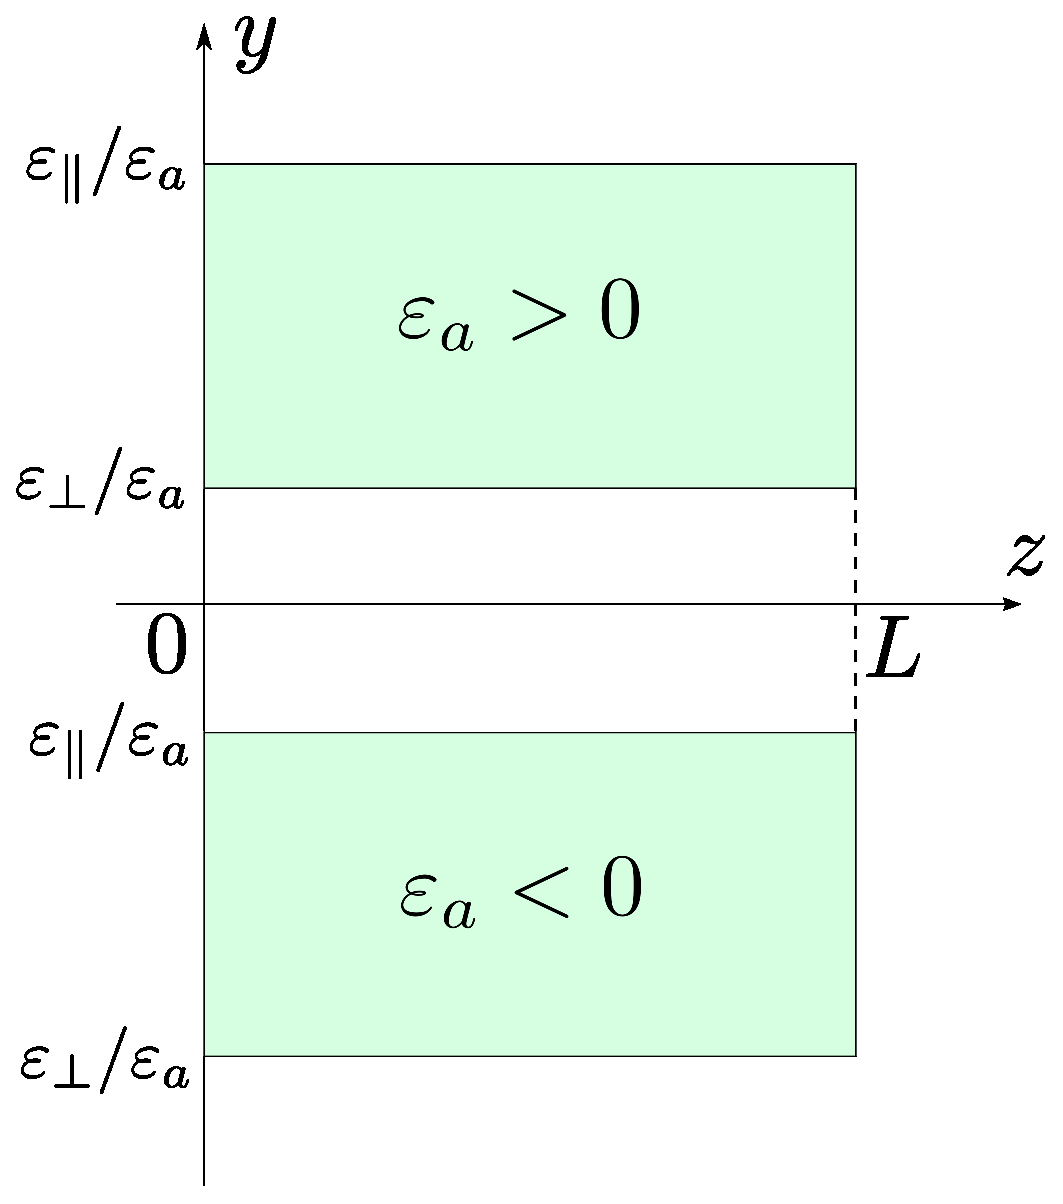
\includegraphics[width=0.55\textwidth]{Allowed_areas_for_y}
	\caption{Графическая иллюстрация системы неравенств~\eqref{eq:rectangle_1}  и~\eqref{eq:rectangle_2} для случаев $\varepsilon_a > 0$ и $\varepsilon_a < 0$.}
\end{figure}
На Рис.~\ref{pic:Allowed_areas_for_y} изображены области, задаваемые неравенствами~\eqref{pic:Allowed_areas_for_y}.
Таким образом, участок кривой $y(z)$ при $z\in[0,\, L]$ должен находиться внутри соответствующего прямоугольника.
Минимум функционалу могут доставлять и такие профили, у которых существуют точки или целые области, где $y(z) = \ve_\|/\ve_a$ или $y(z) = \ve_\bot/\ve_a$.
Обозначим множество таких точек через $A$, а дополнение $A$ до отрезка $[0,L]$ -- $B$.
Проиллюстрируем эти множества на примере графика зависимости $y(
z)$, приведённого на Рис.~\ref{pic:Sample_profile}.
\begin{figure}\label{pic:Sample_profile}
	\centering
	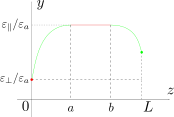
\includegraphics[width=0.7\textwidth]{Sample_profile}
	\caption{График зависимости $y(z)$, иллюстрирующий случай, когда кривая $y(z)$ касается границ ограничивающего прямоугольника.}
\end{figure}
Так, в данном случае $A = \{0\}\cup[a,b]$, $B = (0,a)\cup(b,L]$.
Также важно отметить, что бесконечно малые вариации $\delta y(z)$ произвольны, когда $z\in B$.
В этом случае в условии~\eqref{eq:dF1} может реализоваться только равенство.
Это требование приводит к следующему уравнению Эйлера-Лагранжа:
\begin{align}\label{eq:E-l_y}
&-2yy''+(y')^2 - J^2\left(J_1 - \frac{U}{4\pi\bar{e}}\right)^2 = 0%\\
%&\ve_\bot/\ve_a < y(z) < \ve_\| /\ve_a, \label{cond10}\\
%&0 < z < L.
\end{align}
и граничными условиями
\begin{subequations}
	\begin{align}
		&\bar{e}UJ - 4\pi\bar{e}^2\left( y'(0) + JJ_1 \right) + \ve_a y(0) \frac{W_1}{2} = 0 \label{eq:ch5_boundary1_eq}\\
		-&\bar{e}UJ + 4\pi\bar{e}^2\left( y'(L) + JJ_1 \right) + \ve_a y(L) \frac{W_2}{2} = 0.\label{eq:ch5_boundary2_eq}
	\end{align}
\end{subequations}
Однако при достижении $y(z)$ "верхней" или "нижней" границы прямоугольника~\eqref{eq:rectangle_2}, то есть когда $z\in A$, эти вариации оказываются знакоопределёнными: $\delta y(z) \geq 0$, если $y(z) = \ve_\bot/\ve_a$, и $\delta y(z) \leq 0$ при $y(z) = \ve_\| /\ve_a$.
В этом случае, используя выражение для первой вариации свободной энергии~\eqref{eq:dF_ch5}, для $z\in(0,\ L)\cap A$ вместо уравнения Эйлера-Лагранжа~\eqref{eq:E-l_y} можно записать неравенство
\begin{equation}\label{eq:E-l_ineq}
\left(-2yy''+(y')^2 - J^2\left(J_1 - \frac{U}{4\pi\bar{e}}\right)^2\right)\frac{\delta y}{y} \ge 0.
\end{equation}
Для $z\in \{0, L\}\cap A$ граничные условия также примут форму неравенств:
\begin{subequations}
	\begin{align}
		\left[ -y'(0) - J\left(J_1  - \frac{U}{4\pi\bar{e}}\right) + g_1 y(0) \right]\delta y(0) &\geq 0,\label{eq:boundary1_ch5}\\
		\left[ y'(L) + J\left(J_1  - \frac{U}{4\pi\bar{e}}\right) + g_2 y(L) \right]\delta y(L) &\geq 0,\label{eq:boundary2_ch5}
	\end{align}
\end{subequations}
где
\begin{equation}
g_i = \frac{\ve_a W_i}{8\pi\bar{e}^2},\quad i = 1,2.
\end{equation}
Утверждение.
Если существует некоторый отрезок $[a,\ b] \subset(0,L)$ такой, что множество $[a,b]\cap A$ содержит конечное число элементов, то во всех этих точках $\delta \FF/\delta y = 0$.
Действительно, пусть нашёлся такой отрезок $[a,\ b]$, что существует $z_1$: $z_1\in[a,\ b]\cap A$.
Тогда из непрерывности $\delta \FF/\delta y(z)$ следует, что
\begin{equation}
\frac{\delta \FF}{\delta y(z_1-0)} = \frac{\delta \FF}{\delta y(z_1+0)} = \frac{\delta \FF}{\delta y(z_1)}.
\end{equation}
При этом хотя бы с одной из сторон от $z_1$ $\delta\FF/\delta y(z) = 0$ в силу определения отрезка $[a,\ b]$.
Слеовательно, значение вариации в точке $z_1$ также нулевое.
Утверждение доказано.
	
%Отдельно отметим, что для $z\in\partial A\cap (0,\ L)$ в~\eqref{eq:E-l_ineq} должно выполняться равенство (по непрерывности), а для $z\in\interior{A}$ -- неравенство. 
%Необходимые условия минимума свободной энергии также включают в себя ледующие граничные условия:
%Здесь строгое неравенство соответствует случаю, когда $\{0\}\in A$ или $\{ L \}\in A$, в противном случае имеет место равенство.
При записи условий~\eqref{eq:E-l_ineq}, \eqref{eq:boundary1_ch5} и~\eqref{eq:boundary2_ch5} учтено, что $\ve_a y(z) = \EE(\theta(z)) > 0$.
Отметим, что неравентва~\eqref{eq:E-l_ineq}--\eqref{eq:boundary2_ch5} аналогичны условиям Каруша-Куна-Таккера (см., например,~\cite{Kun-TakkerBook}) для уравнения Эйлера-Лагранжа с граничными условиями.
Таким образом, поиск равновесной ориентационной структуры ЖК-ячейки сводится к достаточно необычной математической задаче: уравнение Эйлера-Лагранжа~\eqref{eq:E-l_y} является интегро-дифференциальным, а также содержит значения искомой функции на границах.
Каждое из граничных условий~\eqref{eq:boundary1_ch5} и~\eqref{eq:boundary2_ch5} -- неравенство и тоже содержит интегральный множитель $J$, зависящий от распределения $\theta(z)$ в объёме ячейки, а также значения $y(0)$ и $y(L)$ в множителе $J_1$.
Наконец, условие, которому должна удовлетворять искомая функция $y(z)$, может быть различным и зависит от того, как распределяются множества $A$ и $B$ на отрезке $[0,\ L]$ для конкретной функции-кандидата. 
%Наконец, если происходит касание границ~\eqref{eq:y_border}, уравнение Эйлера-Лагранжа заменяются неравенством~\eqref{eq:E-l_ineq}.

Достаточное условие минимума свободной энергии может быть получено, если добавить к~\eqref{eq:dF1} требование положительности второй вариации свободной энергии
\begin{equation}
\delta^2\FF[y(z)] > 0,\quad z\in B\cup(\partial A\cap (0,\ L)).
\end{equation}
Во всех остальных точках отрезка $[0,\ L]$ достаточное условие даётся неравенством~\eqref{eq:E-l_ineq}.

Для решения уравнения Эйлера-Лагранжа введём обозначение
\begin{equation}\label{eq:parameter_a}
a = J\left(J_1 - \frac{U}{4\pi\bar{e}}\right).
\end{equation}
Так как выражение $J(J_1 - U/(4\pi\bar{e}))$ не зависит от $z$, получаем параметрическое уравнение
\begin{equation}\label{eq:parametric_EL}
-2yy''+(y')^2 - a^2 = 0.
\end{equation}
Этот параметр также входит в граничные условия~\eqref{eq:boundary1_ch5} и~\eqref{eq:boundary2_ch5}.

Заметим, что если вторая производная  $y''$ равна нулю (а значит, $y(z)$ -- линейная функция), то уравнение~\eqref{eq:parametric_EL} принимает вид
\begin{equation}
(y')^2 - a^2 = 0.
\end{equation}
Семейство линейных функций, являющихся его решениями, может быть описано как
\begin{equation}
y(z) = \pm az + b,
\end{equation}
где $b$ -- произвольная константа.

Далее, путь $y'' \neq 0$.
Введём замену $\tau(y) = y'$.
Тогда справедлива цепочка равенств
\begin{equation}\label{eq:tau_ch5}
y''_{zz} = \tau'_z = \tau'_y y' = \tau'_y\tau.
\end{equation}
Подставляя выражение для $y''$ из~\eqref{eq:tau_ch5} в~\eqref{eq:parametric_EL}, получаем:
\begin{equation}
-2y\tau'_y\tau + \tau^2 - a^2 = 0.
\end{equation}
Разделив переменные и проинтегрировав, запишем
\begin{equation}
\tau^2 - a^2 = cy,
\end{equation}
где $c$ -- произвольная константа.
Учитывая, что $\tau = y'$, проинтегрируем это уравнение:
\begin{equation}
|y'| = \sqrt{cy + a^2} \Rightarrow y = \frac{c}{4}\left( z + b \right)^2- \frac{a^2}{c}.
\end{equation}
Здесь $b$ -- также произвольная константа.

Таким образом, уравнение~\eqref{eq:parametric_EL} имеет три независимых решения
\begin{align}
&y(z) = \pm az + b,\label{eq:linear_solution}\\
&y(z) = \frac{c}{4}\left(z+b\right)^2 - \frac{a^2}{c},\label{eq:parabolic_solution}
\end{align}
где $b$ и $c$ -- произвольные константы.
Выражение~\eqref{eq:parameter_a} является, по своей сути, условием самосогласования на параметр $a$, так как $J$ и $J_1$, в свою очередь, зависят от $a$.
\section{Линейное решение}\label{sec:sec5.1}
Отметим, что из-за требования $y\in C^2[0,\, L]$ кусочно-заданная функция, состоящая из линейных функций~\eqref{eq:linear_solution} решением быть не может.
Подставляя линейное решение~\eqref{eq:linear_solution} в уравнение~\eqref{eq:parametric_EL}, приходим к следующему равенству:
\begin{equation*}
\frac{JU}{4\pi\bar{e}} = 0.
\end{equation*}
Это требование может быть выполнено только в тривиальном случае $U = 0$.
Таким образом, в дальнейшем будем рассатривать только параболическое решение~\eqref{eq:parabolic_solution} с учётом ограничения~\eqref{eq:rectangle_2} на $y(z)$.
Это требование совместно с условиями на границах ячейки~\eqref{eq:boundary1_ch5} и~\eqref{eq:boundary2_ch5}, а также условием самосогласования~\eqref{eq:parameter_a} позволяет определить параметры $a$, $b$ и $c$.
\section{Параболическое решение без участков насыщения}
Проверим возможность существования параболического решения $y(z)$ вида~\eqref{eq:parabolic_solution}, для которого было бы выполнено условие $y(z) \in (\ve_\|/\ve_a,\, \ve_\bot/\ve_a) \forall z\in[0,\, L]$.
На языке множеств $A$ и $B$ этот случай соответствует пустому множеству $B$.
Решение должно обладать следующими свойствами:
\begin{itemize}
	\item Абсцисса вершины параболы находится либо вне отрезка $[0,\, L]$, либо её ордината лежит в области возможных значений функции $y(z)$:
	\begin{subequations}
		\begin{empheq}[left = \empheqlbrack]{align}
			&-b \notin [0,\, L],\\
			&\frac{\ve_\bot}{\ve_a}< \frac{-a^2}{c} < \frac{\ve_\|}{\ve_a};
		\end{empheq}
	\end{subequations}
	\item Значения функции $y(z)$ на краях отрезка $[0,\, L]$ также должны находиться в указанном выше интервале:
	\begin{equation}
		\ve_\bot / \ve_a < y(0,\, L) < \ve_\| / \ve_a
	\end{equation}
	\item Должны быть удовлетворены граничные условия~\eqref{eq:ch5_boundary1_eq} и~\eqref{eq:ch5_boundary2_eq};
	\item Должно выполняться условие самосогласования~\eqref{eq:parameter_a}.
\end{itemize}
Подставим исследуемое параболическое решение в граничные условия~\eqref{eq:ch5_boundary1_eq} и~\eqref{eq:ch5_boundary2_eq} и после несложных преобразований получим:
\begin{subequations}
	\begin{align}
		&\left( b + \frac{2a}{c} \right)\left( \frac{g_1}{2}(b - \frac{2a}{c}) - 1 \right) = 0\label{eq:ch5_boundary1_1}\\
		&\left( L + b + \frac{2a}{c} \right)\left( \frac{g_2}{2}(L + b - \frac{2a}{c}) - 1 \right) = 0.\label{eq:ch5_boundary2_1}
	\end{align}
\end{subequations}
Кроме того, вычисляя $J$ и $J_1$ для $y(z)$ заданного вида, запишем условие самосолгасования~\eqref{eq:parameter_a}:
\begin{multline}
a = a \ve_a \left(\ln{\left( \frac{L+b - 2a/c}{b - 2a/c} \times \frac{b+ 2a/c}{L+b+2a/c} \right)} \right)^{-1} \times\\
\times \left( \frac{1}{\ve_a}\ln{ \left( \frac{b - 2a/c}{L + b - 2a/c} \times \frac{b+ 2a/c}{L+b+2a/c} \right)} - \frac{U}{4\pi\bar{e}} \right).
\end{multline}
После преобразований получаем следующее условие:
\begin{equation}\label{eq:ch5_gamma_1}
	L + b - \frac{2a}{c} = \gamma\left( b - \frac{2a}{c} \right).
\end{equation}
Здесь и далее использовано обозначение
\begin{equation}
	\gamma = \exp{\left(\frac{-\ve_a U}{8\pi\bar{e}}\right)}.
\end{equation}
Видно, что условия~\eqref{eq:ch5_boundary1_1} и~\eqref{eq:ch5_boundary2_1} приводят к равенству нулю одного из множителей в каждом условии.
Рассмотрим теперь значения функции $y(z)$ на границах ячейки:
\begin{subequations}
	\begin{align}
		&y(0) = \frac{c}{2}\left( b-\frac{2a}{c} \right)\left( b + \frac{2a}{c} \right)\\
		&y(L) = \frac{c}{2}\left( L + b - \frac{2a}{c} \right)\left( L + b + \frac{2a}{c} \right)
	\end{align}
\end{subequations}
Из того, что они должны быть отличны от нуля, следует, что в условиях~\eqref{eq:ch5_boundary1_1} и~\eqref{eq:ch5_boundary2_1} нулю могут быть равны только вторые множители, что приводит к следующим равенствам:
\begin{align}
&b - 2a/c = 2/g_1\label{eq:ch5_boundary1_2}\\
&L + b - 2a/c = 2/g_2.\label{eq:ch5_boundary2_2}
\end{align}
Видно, что подстановка~\eqref{eq:ch5_boundary1_2} и~\eqref{eq:ch5_boundary2_2} в~\eqref{eq:ch5_gamma_1} даёт
\begin{equation}
g_1 = \gamma g_2.
\end{equation}
Это выражение связывает материальные параметры и не может быть удовлетворено в общем случае.

Рассмотрим решение параболического типа, для которого множество $B$ содержит единственную точку $z_0$.
Как было показано ранее, если эта точка находится на интервале $(0,\, L)$, то уравнение Эйлера-Лагранжа остаётся в силе, а значит, ничего, по сравнению с предыдущим рассмотренным случаем не меняется.
Таким образом, имеет смысл рассмотреть ситуацию, когда $z_0 = 0$ или $z_0 = L$.
Если эта точка находится на левой границе, $z_0 = 0$, то рассмотрим совместно выражение~\eqref{eq:ch5_gamma_1}, возникающее из условия самосогласования, и равенство~\eqref{eq:ch5_boundary2_2}, возникающее из граничного условия~\eqref{eq:ch5_boundary1_2}:
\begin{subequations}
	\begin{align}
		&L+b-\frac{2a}{c} = \frac{2}{g_2}\\
		&L + b - \frac{2a}{c} = \gamma \left(b - \frac{2a}{c}\right).
	\end{align}
\end{subequations}
Выражая $b - 2a/c$ из каждого из условий и приравнивая полученное, запишем:
\begin{equation}
\frac{2}{g_2} - L = \frac{L}{\gamma - 1}.
\end{equation}
Вновь получено равенство, связывающее материальные параметры, а значит, решение такого типа невозможно. Аналогично можно доказать, что случай $z_0 = L$ тоже не реализуется.

Таким образом, для случая чисто параболического решения остаётся рассмотреть ситуацию, когда на обеих границах отрезка $[0,\, L]$ $y(z)\in\{ \ve_\bot / \ve_a,\, \ve_\| / \ve_a \}$.
Введём обозначения
\begin{equation}
	y(0,\, L) = \mu_{0,\, L}.
\end{equation}
Можно записать все условия, которым должно удовлетворять решение:
\begin{subequations}
	\begin{empheq}[left = \empheqlbrace]{align}
		&y(z) = \frac{c}{4}(z + b)^2 - \frac{a^2}{c},\label{eq:ch5_parabolic_system_1}\\
		&y(0) = \mu_0,\label{eq:ch5_parabolic_system_2}\\
		&y(L) = \mu_L,\label{eq:ch5_parabolic_system_3}\\
		&a = J\left(J_1 - \frac{U}{4\pi\bar{e}}\right),\label{eq:ch5_parabolic_system_4}\\
		&\left[\begin{aligned}
			&-b \notin [0,\, L],\\
			&\frac{\ve_\bot}{\ve_a}< \frac{-a^2}{c} < \frac{\ve_\|}{\ve_a},
		\end{aligned}\right.,\label{eq:ch5_parabolic_system_5}\\
		&\left[ -(y'(0) + a) + g_1 y(0) \right]\delta y(0) \geq 0,\label{eq:ch5_parabolic_system_6}\\
		&\left[ y'(L) + a + g_2 y(L) \right]\delta y(L) \geq 0.\label{eq:ch5_parabolic_system_7}
	\end{empheq}
\end{subequations}
Подстановка зависимости~\eqref{eq:ch5_parabolic_system_1} в~\eqref{eq:ch5_parabolic_system_2}, \eqref{eq:ch5_parabolic_system_3} и~\eqref{eq:ch5_parabolic_system_4} даёт следующую систему уравнений на коэффициенты $a$, $b$ и $c$: \todo{(эта система взята со страницы R-2)}
\begin{subequations}
	\begin{empheq}[left = \empheqlbrace]{align}
		&b = -\frac{L}{2}\left( \frac{\pm \gamma}{\frac{\mu_L}{\mu_0} \pm \gamma} + \frac{1}{1\pm \gamma} \right),\\
		&b - \frac{2a}{c} = \frac{-L}{1 \pm \gamma},\\
		&\frac{c}{4} \cdot \frac{-L}{1 \pm \gamma}\left( b + \frac{2a}{c} \right) = \mu_0.
	\end{empheq}
\end{subequations}
Здесь и далее подразумевается, что во всех выражениях могут стоять одновременно либо только ``верхние'', либо только ``нижние'' знаки.
После несложных алгебраических преобразований удаётся выразить следующие конструкции из коэффициентов, удобные для дальнейшей подстановки:
\begin{subequations}\label{eq:ch5_parabolic_coeff_system}
	\begin{empheq}[left = \empheqlbrace]{align}
		&b = \frac{-L}{2}\left( \frac{\pm \gamma}{\frac{\mu_L}{\mu_0} \pm \gamma} + \frac{1}{1 \pm \gamma}\right),\label{eq:ch5_parabolic_coeff_system_1}\\
		&\frac{2a}{c} = \frac{L}{2}\left( \frac{1}{1 \pm \gamma} - \frac{\pm \gamma}{\frac{\mu_L}{\mu_0} \pm \gamma} \right),\label{eq:ch5_parabolic_coeff_system_2}\\
		&\frac{c}{4} = \frac{\mu_0 \left(1 \pm \gamma\right)\left( \frac{\mu_L}{\mu_0} \pm \gamma \right)}{\pm \gamma L^2}.\label{eq:ch5_parabolic_coeff_system_3}
	\end{empheq}
\end{subequations}
Граничные условия~\eqref{eq:ch5_parabolic_system_6} и~\eqref{eq:ch5_parabolic_system_7} после подстановки в них выражений для коэффициентов~\eqref{eq:ch5_parabolic_coeff_system_1} -- \eqref{eq:ch5_parabolic_coeff_system_3} принимают следующий вид:
\begin{subequations}\label{eq:ch5_some_system}
	\begin{empheq}[left = \empheqlbrace]{align}
		&\mu_0\left( g_1 + \frac{2(1 \pm \gamma)}{L} \right) \delta y(0) \geq 0,\label{eq:ch5_some_system_a}\\
		&\mu_L \left( g_2 + \frac{2(1 \pm \gamma^{-1})}{L} \right) \delta y(L) \geq 0.\label{eq:ch5_some_system_b}
	\end{empheq}
\end{subequations}
\todo{АО: надо придумать, как здесь заменить $\delta y(0,\, L)$ на единицу в некоторой степени.}
Для того, чтобы анализа полученные неравенства, необходимо выбрать знаки $\ve_a$ и $U$.
Произведём расчёт для случая $\ve_a > 0$, $U > 0$.
Заметим, что в этом случае выполнены следующие неравества:
\begin{subequations}
	\begin{align}
		&\mu_{0,L} > 0,\label{eq:ch5_conseq_from_positive_ea_U_1}\\
		&0 < \gamma \leq 1,\label{eq:ch5_conseq_from_positive_ea_U_2}\\
		&1 \leq \gamma^{-1} < \infty.\label{eq:ch5_conseq_from_positive_ea_U_3}
	\end{align}
\end{subequations}
Учитывая требование~\eqref{eq:ch5_conseq_from_positive_ea_U_2}, неравенство~\eqref{eq:ch5_some_system_a} можно свести к требованию $\delta y(0) > 0$, что соответствует $\mu_0 = \ve_\bot / \ve_a$.
Предположим, что знак при $\gamma$ -- ``верхний''.
Тогда неравенство~\eqref{eq:ch5_some_system_b} принимает вид
\begin{equation}
	\left( g_2 + \frac{2(1 + \gamma^{-1})}{L} \right) \delta y(L) \geq 0.
\end{equation}
Выражение в скобках может принимать только положительные значения ($g_{1,2} > 0$, так как $\ve_a > 0$).
Таким образом, приходим к требованию $\delta y(L) > 0$, что соответствует $\mu_L = \mu_0 = \ve_\bot / \ve_a$.
Так как $y(0) = y(L)$, вершина параболы находится в точке $z = L/2$, а значит, нужно проверить, не выходит ли ордината вершины за границы допустимого отрезка.
Выражение для ординаты параболы:
\begin{equation}\label{eq:ch5_ordinate_of_vertex_symmetric}
	y(z)\bigg|_{z = -b} = \frac{-a^2}{c},
\end{equation}
на него наложено следующее ограничение:
\begin{equation}\label{eq:ch5_case1_ineq_system}
	\frac{\ve_\bot}{\ve_a} \leq \frac{-a^2}{c} \leq \frac{\ve_\|}{\ve_a}.
\end{equation}
Воспользуемся полученными ранее формулами~\eqref{eq:ch5_parabolic_coeff_system}, чтобы выразить $-a^2/c$, и после несложных преобразований получим
\begin{equation}\label{eq:ch5_case_low_sign_ineq}
	1 \leq \frac{-(1 - \gamma)^2}{4\gamma}\leq \frac{\ve_\|}{\ve_\bot}.
\end{equation}
Видно, что это условие не выполняется, а значит, решений в случае выбранного при $\gamma$ знака при $\ve_a > 0$ и $U > 0$ нет.

Рассмотрим теперь ``нижний'' знак при $\gamma$.
В этом случае неравенство~\eqref{eq:ch5_some_system_b} принимает вид
\begin{equation}\label{eq:ch5_right_border_ineq}
	\left( g_2 + \frac{2(1 - \gamma^{-1})}{L} \right) \delta y(L) \geq 0.
\end{equation}
Знак выражения в скобках определяет, какого знака должна быть вариация $\delta y(L)$.
Заметим, что с ростом $U$ значение $\gamma^{-1}$ также монотонно растёт.
Следовательно, существует некоторое значение напряжения $U = \tilde{U}$ такое, что при $U < \tilde{U}$, $\delta y(L) > 0$, а при $U > \tilde{U}$, $\delta y(L) < 0$.
Найти напряжение $\tilde{U}$ можно, приравнивая значение выражения в скобках в формуле~\eqref{eq:ch5_right_border_ineq} к нулю.
После несложных преобразований получим:
\begin{equation}
	\tilde{U} = \frac{8\pi \bar{e}}{\ve_a} \ln \left( 1 + \frac{\ve_a W_2 L}{16\pi \bar{e}^2} \right).
\end{equation}
Рассмотрим случай  $U < \tilde{U}$.
Как сказано выше, это условие приводит к тому, что $\mu_L = \ve_\bot / \ve_a$.
Проверим, выполняется ли условие на ординату вершины параболы, которая при $\mu_0 = \mu_L$ имеет абсциссу $z = -b$.
Подставим в~\eqref{eq:ch5_ordinate_of_vertex_symmetric} выражения для комбинации коэффициентов из~\eqref{eq:ch5_parabolic_coeff_system}:
\begin{equation}
	y(z)\bigg|_{z = -b} = -\left( \frac{2a}{c} \right)^2 \cdot \frac{c}{4} = \frac{\mu_0 \left( \frac{\mu_L}{\mu_0} - \gamma^2 \right)^2}{4\gamma\left(1-\gamma\right)\left( \frac{\mu_L}{\mu_0} - \gamma \right)}.
\end{equation}
Подставляя полученные выше значения $\mu_0 = \mu_L = \ve_\bot / \ve_a$, запишем условие на вершину параболы:
\begin{equation}\label{eq:ch5_toomanynames_001}
	1 \leq \frac{(1+\gamma)^2}{4\gamma} \leq \frac{\ve_\|}{\ve_\bot}.
\end{equation}
Видно, что первое неравенство в~\eqref{eq:ch5_toomanynames_001} выполнено для всех $\gamma\in(0,\, 1]$, а вот второе является содержательным.
Исследуем неравенство
\begin{equation}\label{eq:ch5_case_1_ineq}
(1+\gamma)^2 \leq \frac{4\gamma\ve_\|}{\ve_\bot}.
\end{equation}
Графики функций $f_1(\gamma) = (1+\gamma)^2$ и $f_2(\gamma) = 4\gamma\ve_\|/\ve_\bot$ представлены на Рис.~\ref{fig:ch5_graph_solver_1}
\begin{figure}[h]
	\centering
	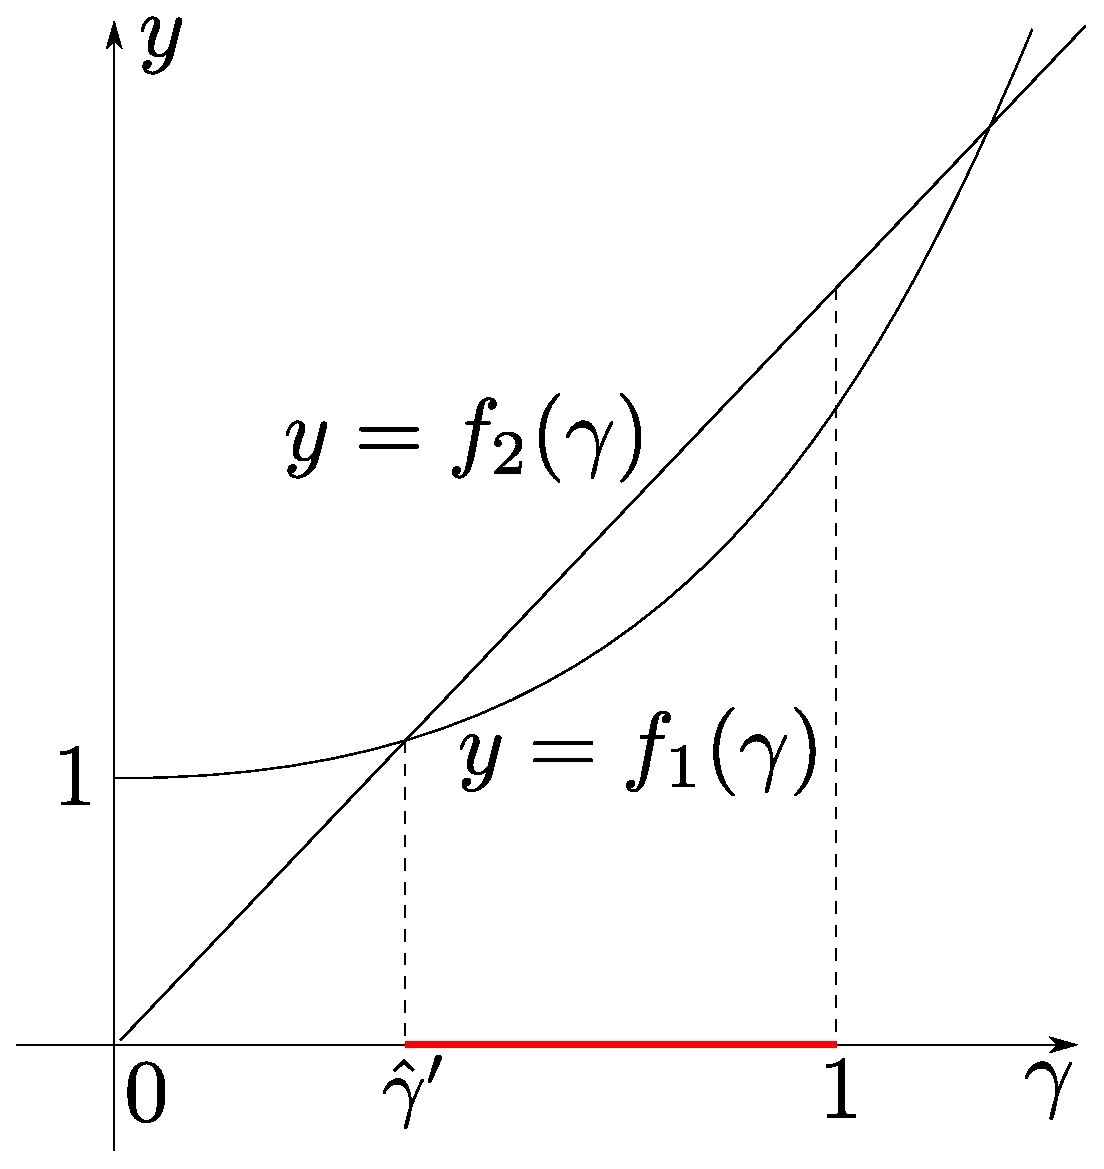
\includegraphics[width=20pc]{ch5_graph_solver_1.eps}
	\caption{Графики функций $y = f_1(\gamma)$ и $y = f_2(\gamma)$. Цветом выделен участок на оси $\gamma$, соответствующий решению неравенства~\eqref{eq:ch5_case_1_ineq}.}\label{fig:ch5_graph_solver_1}
\end{figure}
При построении графиков учтено, что $f_2(0) < f_1(0)$ и $f_2(1) > f_1(1)$, следовательно, на интервале $(0,\, 1)$ существует $\hat{\gamma}'$ такая, что $f_1(\hat{\gamma}') = f_2(\hat{\gamma}')$.
При этом неравенство~\eqref{eq:ch5_case_1_ineq} выполнено при $\hat{\gamma}' < \gamma \leq 1$, что в терминах напряжений соответствует $0 \leq U < \hat{U}'$, $\hat{U}':\hat{\gamma}' = \gamma(\hat{U}')$.
Приведём точное выражение для $\hat{\gamma}'$ и соответствующего напряжения $\hat{U}'$:
\begin{align}
	&\hat{\gamma}' = \frac{2\ve_\|}{\ve_\bot} - 1 - \frac{2\ve_\|}{\ve_\bot} \sqrt{\frac{\ve_a}{\ve_\|}},\\
	&\hat{U}' = \frac{8\pi\bar{e}}{\ve_a}\ln\left( \frac{1}{\hat{\gamma}'} \right).
\end{align}
Напомним, что условие $U < \tilde{U}$ соответствует неравенству, заменяющему граничное условие на границе $z = L$, а условие $U < \hat{U}'$ соответствует требованию, чтобы вершина параболы не выходила за гарницы обозначенного прямоугольника.

Таким образом, заключаем, что при $U < \min(\tilde{U},\,\hat{U}_1)$ возможно существование профиля, изображённого на Рис.~\ref{fig:ch5_profile_1}.
\begin{figure}
	\centering
	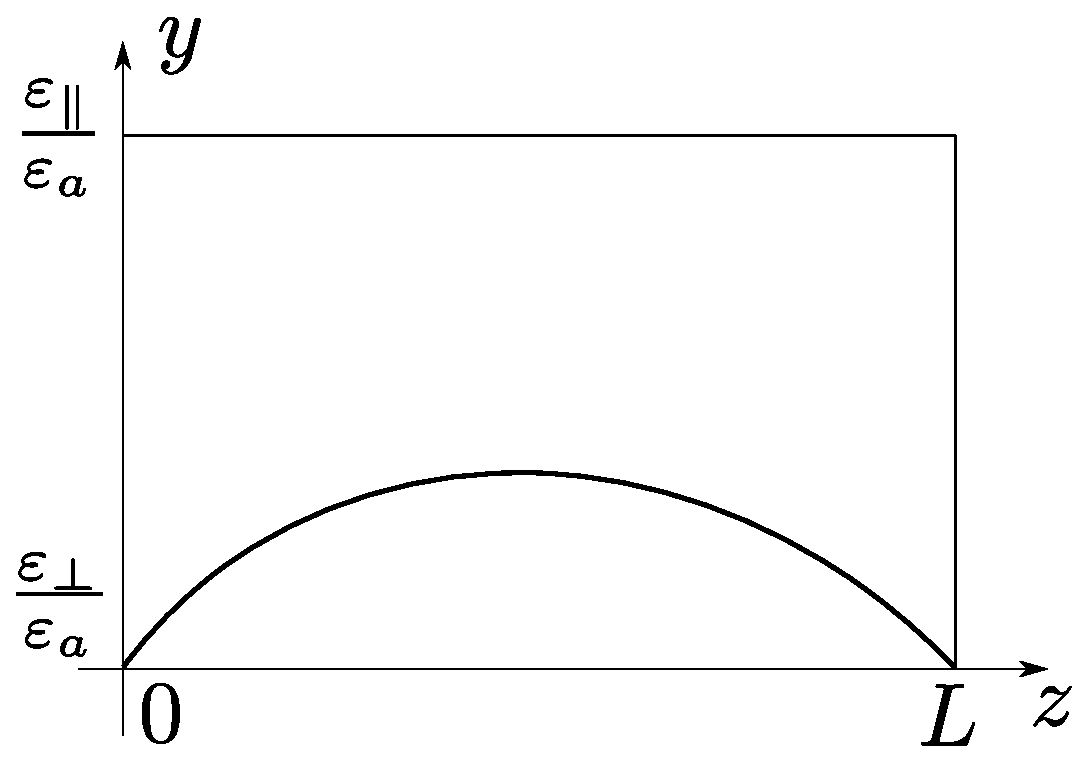
\includegraphics[width = 17pc]{ch5_profile_1.eps}
	\caption{Вид профиля при напряжении $U < \min(\tilde{U},\,\hat{U}_1)$}\label{fig:ch5_profile_1}
\end{figure}
Подставляя $\mu_0 = \mu_L = \ve_\bot/\ve_a$ в~\eqref{eq:ch5_parabolic_coeff_system} и выбирая ``нижний'' знак при $\gamma$, можно получить уравнение такого профиля:
\begin{equation}\label{eq:ch5_simple_parabolic_profile}
	y(z) = \frac{\ve_\bot}{\ve_a}\cdot\frac{(1 - \gamma)^2}{-\gamma^2}\cdot\left( \frac{z}{L}  - \frac{1}{2} \right)^2 + \frac{\ve_\bot}{\ve_a}\cdot \frac{(1 + \gamma)^2}{4\gamma}
\end{equation}

Мы рассмотрели случай $U < \tilde{U}$, что приводит к $\mu_L = \ve_\bot / \ve_a$.
Рассмотрим теперь $U > \tilde{U}$.
В свою очередь, это условие приводит к требованию $\mu_L = \ve_\|/\ve_a$.
Такие значения $\mu_0$ и $\mu_L$ приводят к профилям, схематически изображённым на Рис.~\ref{fig:ch5_profile_2}.
\begin{figure}
	\centering
	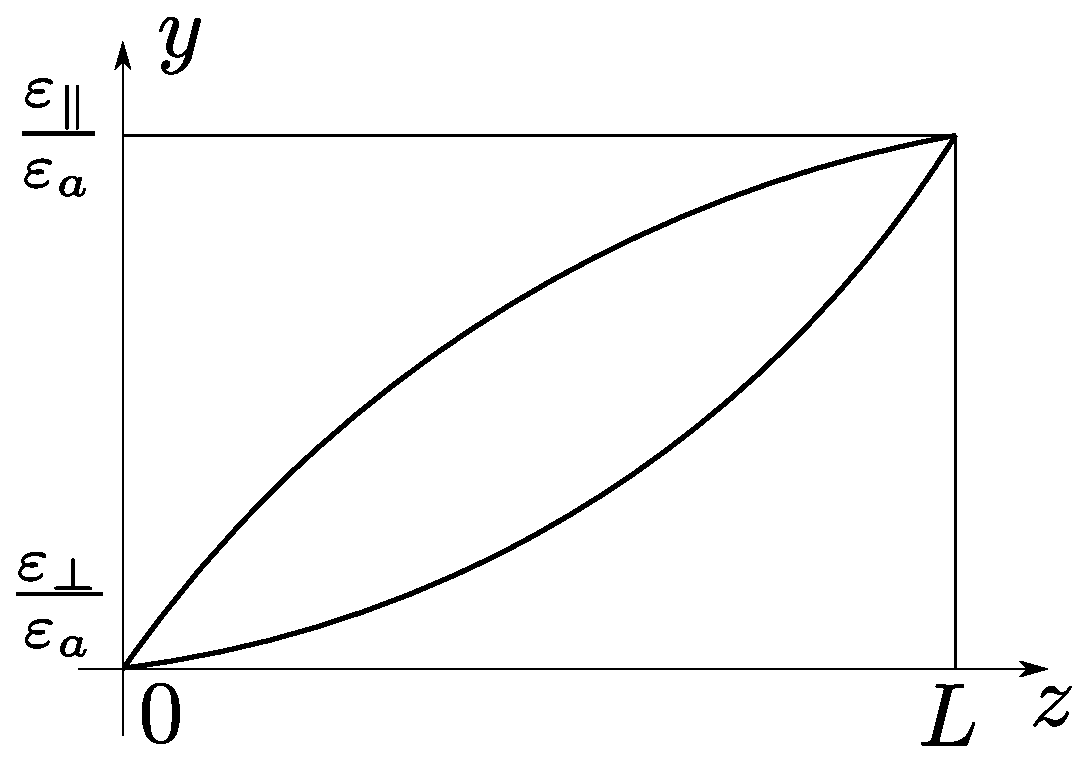
\includegraphics[width = 17pc]{ch5_profile_2.eps}
	\caption{Схематическое изображение параболических профилей без участков насыщения при $\mu_0 = \ve_\bot/\ve_a$ и $\mu_L = \ve_\|/\ve_a$.}\label{fig:ch5_profile_2}
\end{figure}
Проверим, при каких значениях напряжения $U$ выполнено условие на вершину параболы.
В данном случае может быть выполнено только первое условие из совокупности~\eqref{eq:ch5_parabolic_system_5}.
Подставляя в выражение для коэффициента $b$~\eqref{eq:ch5_parabolic_coeff_system_1} ``нижний'' знак при $\gamma$ и исследуемые значения $\mu_{0, L}$, запишем первое условие  из~\eqref{eq:ch5_parabolic_system_5}:
\begin{subequations}
	\begin{empheq}[left = \empheqlbrack]{align}
		&\frac{L}{2}\left( \frac{-\gamma}{\frac{\ve_\|}{\ve_\bot} - \gamma} + \frac{1}{1 - \gamma} \right) < 0,\label{eq:ch5_system_2_a}\\
		&\frac{L}{2}\left( \frac{-\gamma}{\frac{\ve_\|}{\ve_\bot} - \gamma} + \frac{1}{1 - \gamma} \right) > L.\label{eq:ch5_system_2_b}
	\end{empheq}
\end{subequations}
Рассмотрим неравенство~\eqref{eq:ch5_system_2_a}.
После несложных преобразований можно прийти к следующей записи:
\begin{equation}\label{eq:ch5_case_2_ineq_1}
	\frac{1}{1 - \gamma} < \frac{\gamma}{\frac{\ve_\|}{\ve_\bot} - \gamma}
\end{equation}
Заметим, что $\ve_\|/\ve_\bot > 1$ (так как рассматривается случай $\ve_a > 0$), а $\gamma < 1$.
Отсюда можно сделать вывод, что неравенство~\eqref{eq:ch5_case_2_ineq_1} не может быть выполнено.
Отсюда также следует, что профиль, обозначенный на Рис.~\ref{fig:ch5_profile_2} пунктирной линией, не может быть равновесным.

Рассмотрим неравенство~\eqref{eq:ch5_system_2_b}.
Его при помощи алгебраических преобразований можно свести к следующему виду:
\begin{equation}\label{eq:ch5_case_2_ineq_2}
	(1 - \gamma)^2 < (2\gamma -1)\frac{\ve_a}{\ve_\bot}.
\end{equation}
Графики функций $f_1(\gamma) = (1-\gamma)^2$ и $f_2(\gamma) = (2\gamma - 1)\ve_a/\ve_\bot$ представлены на Рис.~\ref{fig:ch5_graph_solver_2}.
\begin{figure}[h]
	\centering
	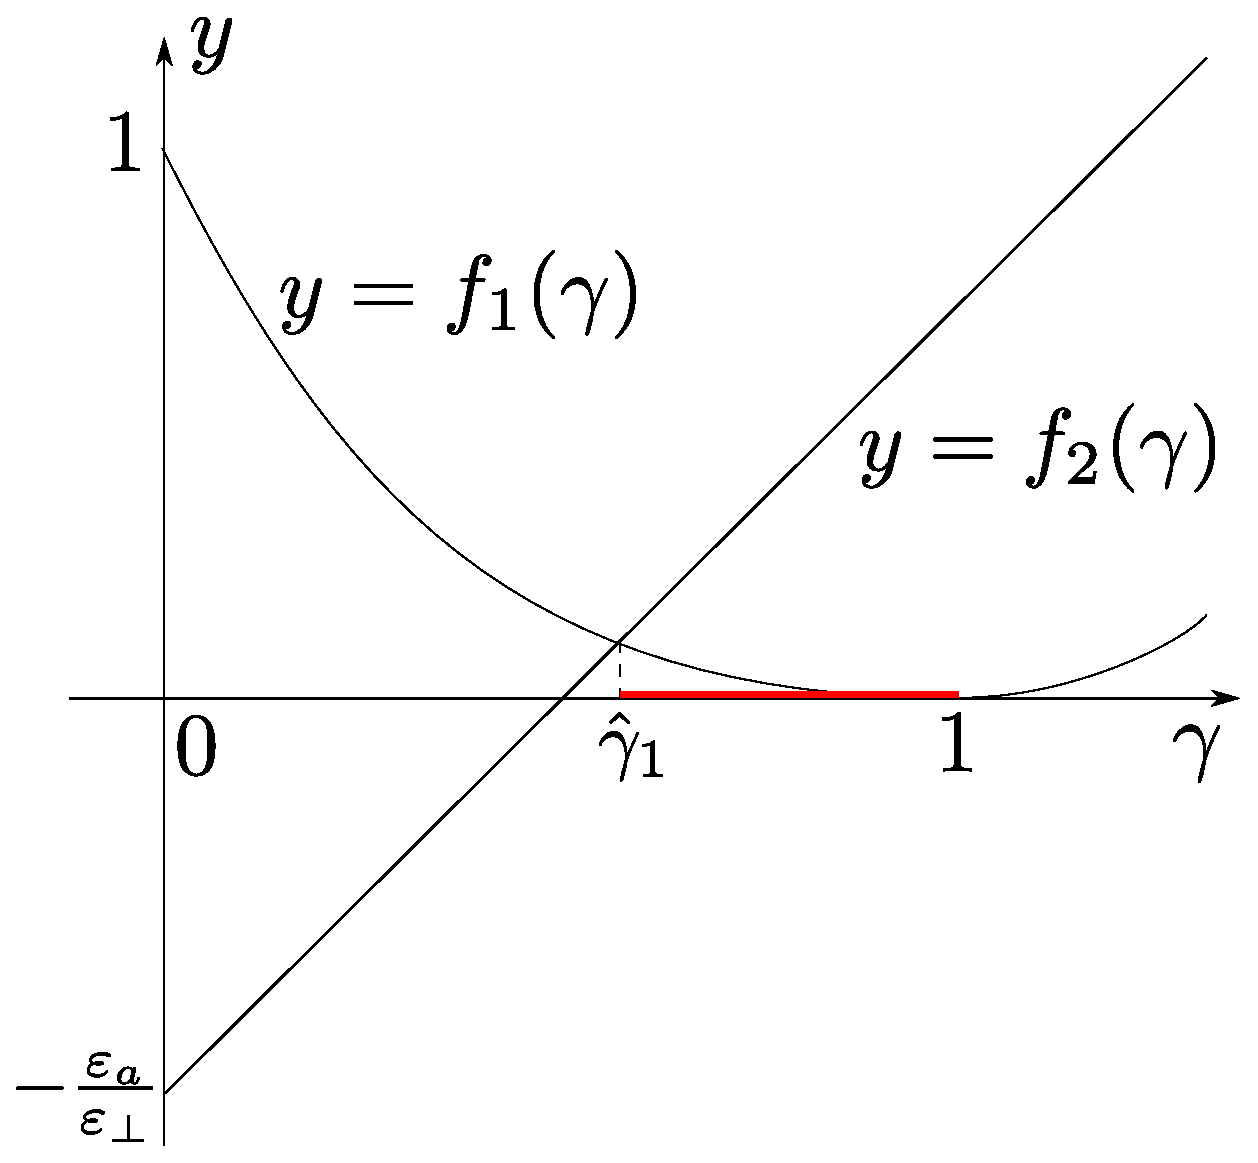
\includegraphics[width=20pc]{ch5_graph_solver_2.eps}
	\caption{Графики функций $y = f_1(\gamma)$ и $y = f_2(\gamma)$. Цветом выделен участок на оси $\gamma$, соответствующий решению неравенства~\eqref{eq:ch5_case_2_ineq_2}.}\label{fig:ch5_graph_solver_2}
\end{figure}
Здесь при построении графика учтено, как соотносятся значения обеих функций при $\gamma = 0$ и $\gamma = 1$.
Таким образом, неравенство~\eqref{eq:ch5_case_2_ineq_2} выполнено, когда $\gamma\in(\hat{\gamma}_1,\,1]$, что соответствует $U\in[0,\, \hat{U}_1)$.
Решая квадратное уравнение, можно получить точное выражение для $\hat{\gamma}_1$ и напряжения $\hat{U}_1$:
\begin{align}
	&\hat{\gamma}_1 = \frac{\ve_\|}{\ve_\bot} - \frac{\ve_\|}{\ve_\bot}\sqrt{\frac{\ve_a}{\ve_\|}},\\
	&\hat{U}_1 = \frac{8\pi \bar{e}}{\ve_a}\ln\left( \frac{1}{\hat{\gamma}_1} \right)
\end{align}
Вновь, условие $U > \tilde{U}$ отвечает за выполнение неравенства~\eqref{eq:ch5_right_border_ineq} на правой границе, а условие $U < \hat{U}_1$ порождено требованием на вершину параболы.

Таким образом, можно видеть, что при
\begin{equation}\label{eq:ch5_case_2_ineq_3}
\tilde{U} < U < \hat{U}_1
\end{equation}
равновесной будет ориентационная структура, профиль $y(z)$ которой обозначен на Рис.~\ref{fig:ch5_profile_2} сплошной линией.
Подставляя в~\eqref{eq:ch5_parabolic_system_1} выражения для коэффициентов~\eqref{eq:ch5_parabolic_coeff_system} с учётом $\mu_0 = \ve_\bot/\ve_a$, $\mu_L = \ve_\|/\ve_a$ и ``нижнего'' при $\gamma$, получим уравнение этого профиля в явном виде:
\begin{multline}\label{eq:ch5_asymmetric_parabolic_profile}
	y(z) = -\frac{\ve_\bot}{\ve_a}\cdot\frac{(1-\gamma)\left(\frac{\ve_\|}{\ve_\bot} - \gamma \right)}{\gamma}\left[ \frac{z}{L} - \frac{1}{2}\cdot\frac{(1 - \gamma)^2 + \frac{\ve_a}{\ve_\bot}}{(1 - \gamma)\left( \frac{\ve_\|}{\ve_\bot} - \gamma \right)} \right] +\\
	+ \frac{\ve_\bot}{\ve_a}\cdot\frac{\left( \frac{\ve_\|}{\ve_\bot} - \gamma^2 \right)^2}{\gamma(1-\gamma)\left( \frac{\ve_\|}{\ve_\bot} - \gamma \right)}.
\end{multline}

Заметим, что для того, чтобы интервал напряжений, задаваемый двойным неравенством~\eqref{eq:ch5_case_2_ineq_3}, был непустым, также необходимо, чтобы выполнялось следующее неравенство:
\begin{equation}
	\tilde{U} < \hat{U}_1
\end{equation}
Для дальнейшего анализа удобно ввести обозначение
\begin{equation}
	\varkappa = \sqrt{\frac{\ve_\|}{\ve_a}}
\end{equation}
и записать найденные выше характеристические напряжения $\tilde{U}$, $\hat{U}'$ и $\hat{U}_1$ с его помощью:
\begin{subequations}\label{eq:ch5_case_2_ineqs_4}
	\begin{align}
		&\tilde{U} = \frac{8\pi\bar{e}}{\ve_a}\ln\left( 1 + \frac{g_2 L}{2} \right),\\
		&\hat{U}' = \frac{8\pi\bar{e}}{\ve_a}\ln\frac{\varkappa + 1}{\varkappa - 1},\\
		&\hat{U}_1 = \frac{8\pi\bar{e}}{\ve_a}\ln\frac{\varkappa + 1}{\varkappa}.
	\end{align}
\end{subequations}
Отметим, что $\hat{U}_1 < \hat{U}'$.
Значит, остаётся три возможных варианта взаимного расположения напряжений:
\begin{subequations}
	\begin{align}
		&\hat{U}_1 < \hat{U}' < \tilde{U},\\
		&\hat{U}_1 < \tilde{U} < \hat{U}',\\
		&\tilde{U} < \hat{U}_1 < \hat{U}'.
	\end{align}
\end{subequations}
С учётом явно выраженный напряжений~\eqref{eq:ch5_case_2_ineqs_4} эти неравенства можно переписать следующим образом:
\begin{subequations}\label{eq:ch5_case_2_ineqs_5}
	\begin{align}
		&\frac{2}{\varkappa} < \frac{4}{\varkappa - 1} < g_2 L,\label{eq:ch5_case_2_ineqs_5_a}\\
		&\frac{2}{\varkappa} < g_2 L < \frac{4}{\varkappa - 1},\label{eq:ch5_case_2_ineqs_5_b}\\
		&g_2 L < \frac{2}{\varkappa} < \frac{4}{\varkappa - 1}.\label{eq:ch5_case_2_ineqs_5_c}
	\end{align}
\end{subequations}
Видно, что параметром, который отвечает за то, какой сценарий будет реализован в данной системе (при данном наборе параметров), является $g_2 L$.
Выясним, каким именно сценариям трансформации ориентационной структуры с изменнением $U$ соответствуют ситуации~\eqref{eq:ch5_case_2_ineqs_5}.
\begin{itemize}
	\item Случай ``сильного'' сцепления, $2/\varkappa < g_2 L$.
	
	При таких значениях параметра $g_2 L$ будет реализован сценарий, схематически изображённый на Рис.~\ref{fig:ch5_scheme_nonsaturated_part_1}.
	\begin{figure}[h]
		\centering
		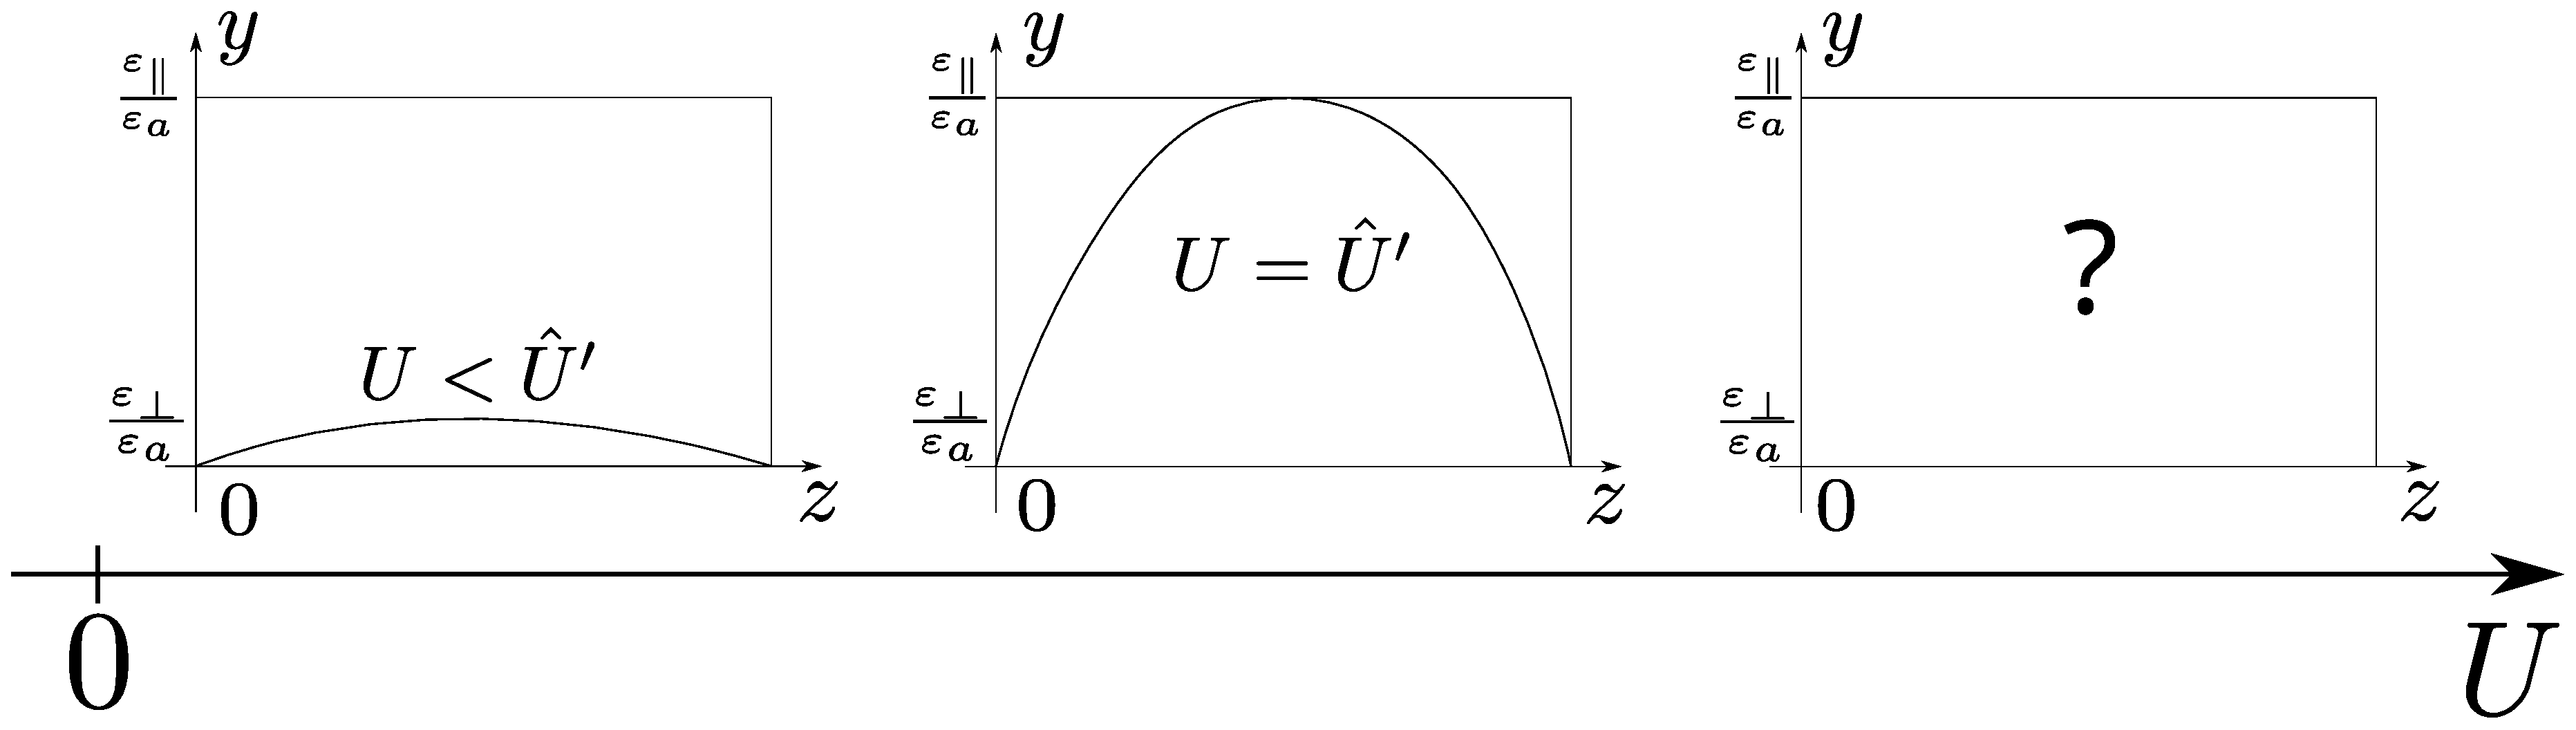
\includegraphics[width=\textwidth]{ch5_scheme_nonsaturated_part_1.eps}
		\caption{Схематическое изображение трансформации профилей $y(z)$ с ростом приложенного напряжения $U$ в случае ``сильного'' сцепления, задаваемого неравенством~\eqref{eq:ch5_case_2_ineqs_5_a}.}\label{fig:ch5_scheme_nonsaturated_part_1}
	\end{figure}
	Видно, что с ростом $U$ от $U = 0$ сначала происходит небольшое искажение структуры вблизи середины ячейки, затем это искажение распространяется ближе к границам и становится всё сильнее.
	При этом ориентация на обеих границах остаётся планарной.
	Наконец, профиль $y(z)$ касается ``верхней границы'' в середине ячейки при $U = \hat{U}'$.
	Дальнейшая эволюция ориентационной структуры ЖК требует рассмотрения профилей с участками насыщения, что будет проделано в части~\ref{sec:sec5.1}.
	На данном этапе эти стадии эволюции отмечены знаками вопроса.
	Отметим, что здесь и на остальных аналогичных схемах по оси напряжений отсутствует масштаб, она нанесена, чтобы показать, в каком порядке сменяются профили с ростом $U$.
	Кроме того, можно увидеть, что в данном сценарии не упоминается напряжение $\hat{U}_1$.
	Это происходит из-за того, что оно соответствует нарушению условия на вершину параболы для асимметричного профиля без участков насыщения, который в данном случае не может быть равновесным.

	\item Случай ``среднего'' сцепления, $4/(\varkappa - 1) < g_2 L < 2/\varkappa$.
	
	При данных значениях параметра $g_2 L$, характеризующего сцепление с подложкой, реализуется сценарий, схематиччески изображённый на Рис.~\ref{fig:ch5_scheme_nonsaturated_part_2}.
	\begin{figure}[h]
		\centering
		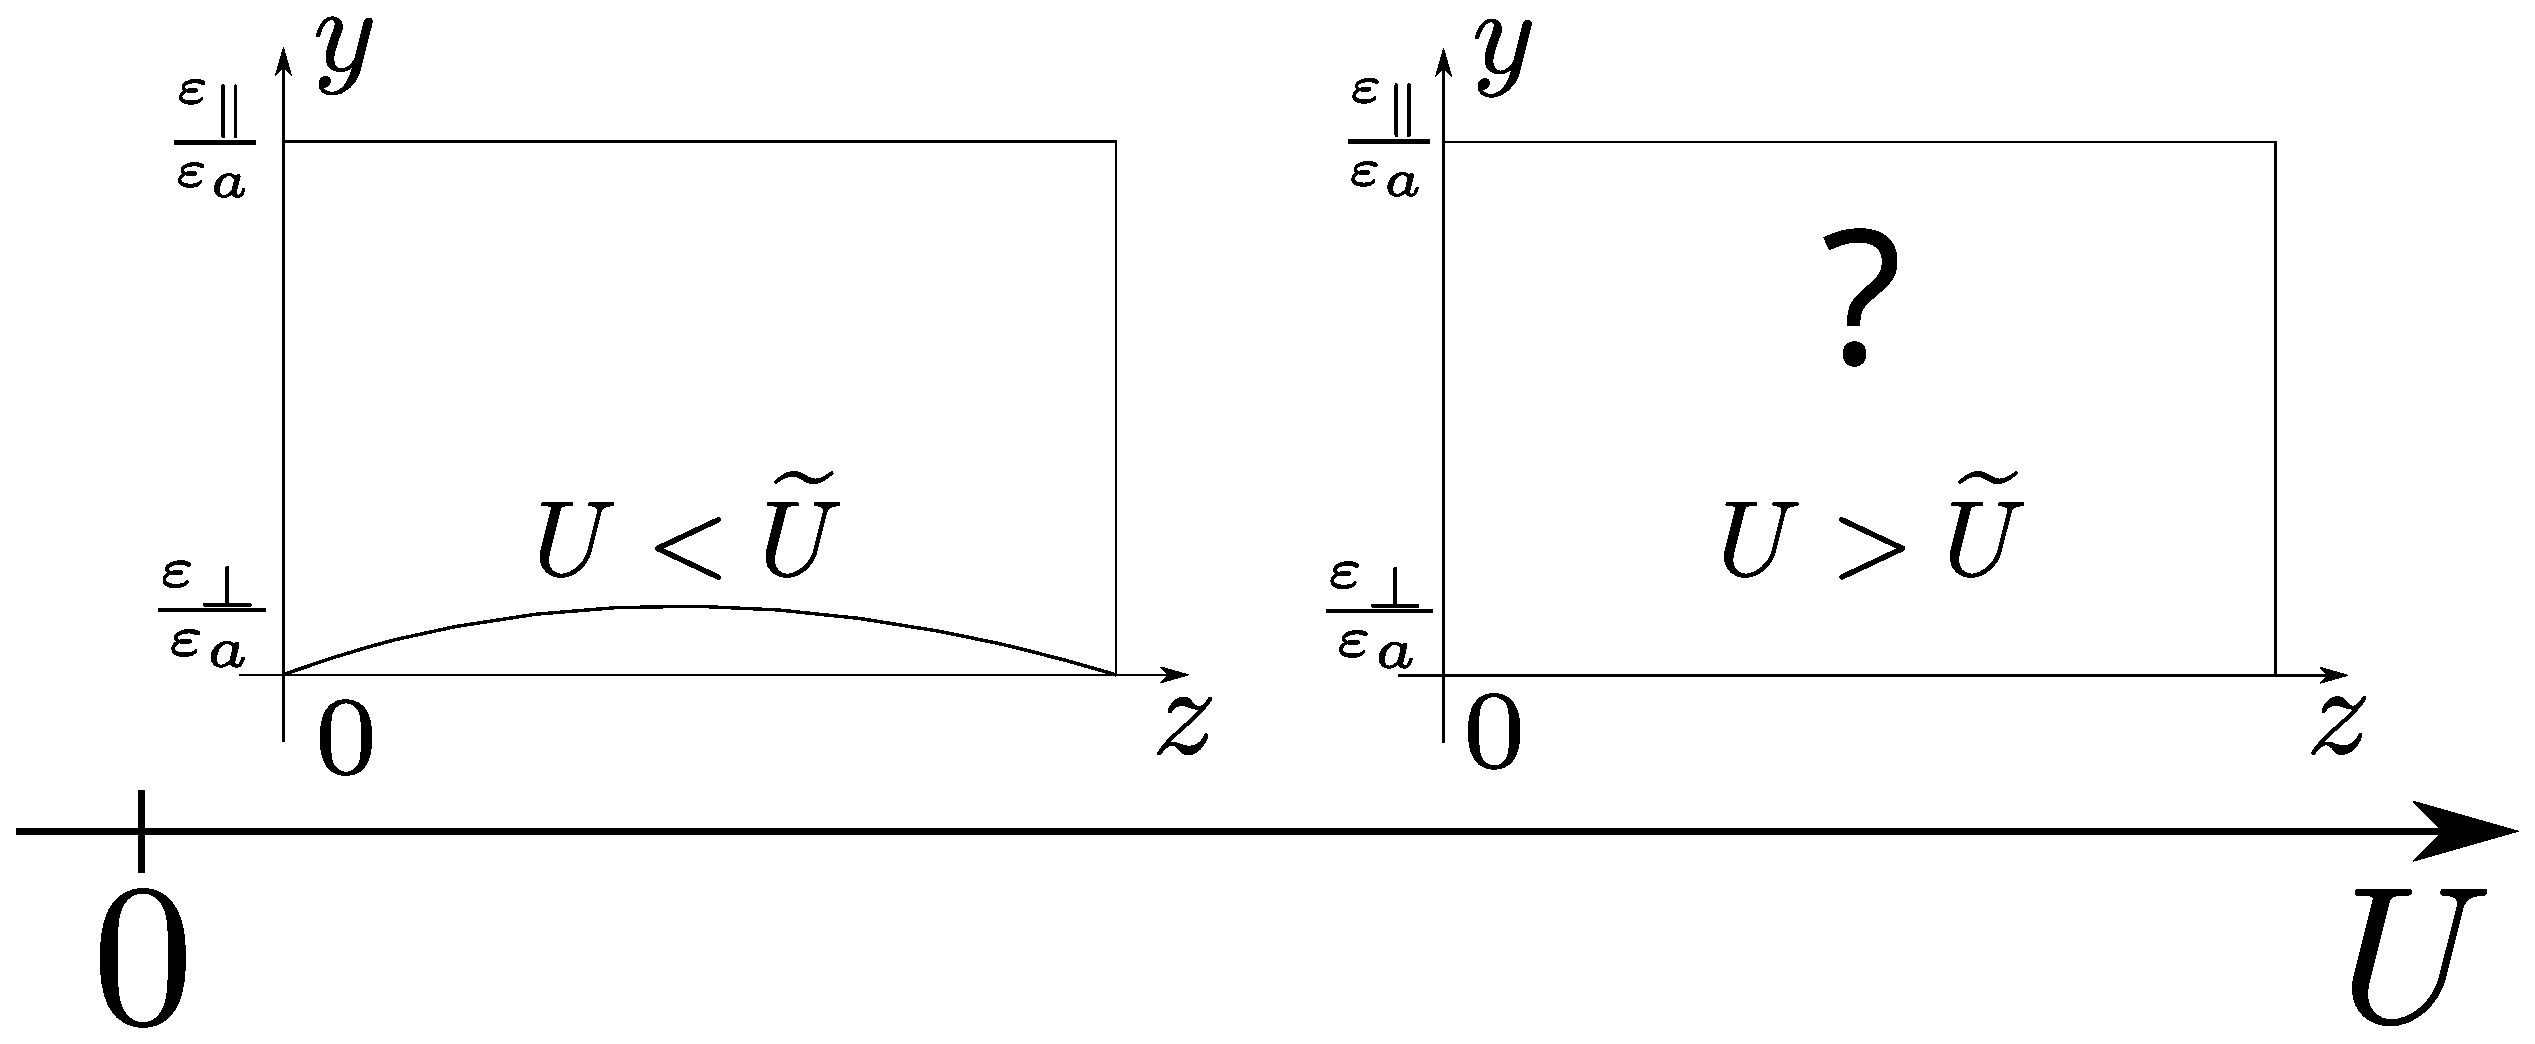
\includegraphics[width=0.7\textwidth]{ch5_scheme_nonsaturated_part_2.eps}
		\caption{Схематическое изображение трансформации профилей $y(z)$ с ростом приложенного напряжения $U$ в случае ``среднего'' сцепления, задаваемого неравенством~\eqref{eq:ch5_case_2_ineqs_5_b}.}\label{fig:ch5_scheme_nonsaturated_part_2}
	\end{figure}
	В этом случае единственным возможным решением без участков насыщения является профиль, задаваемый уравнением~\eqref{eq:ch5_simple_parabolic_profile}.
	Это происходит из-за того, что симметричный (относительно $z = L/2$) параболический профиль является равновесным, пока выполнено неравенство
	\begin{equation}
		U < \min(\tilde{U}, \hat{U}'),
	\end{equation}
	которое в данном случае сводится к $U < \tilde{U}$.
	Поясним, почему в данном случае при рассмотрении изменения ориентационной структуры с ростом $U$ мы не упоминаем напряжения $\hat{U}_1$ и $\hat{U}'$.
	Напряжение $\hat{U}'$ отвечает за касание вершиной симметричного параболического профиля верхней границы, $\ve_\|/\ve_a$ (эта ситуация изображена на второй диаграмме на Рис.~\ref{fig:ch5_scheme_nonsaturated_part_2}), однако этого произойти не может, так как сначала будет достигнуто напряжение $\tilde{U}$, и условие на правой границе~\eqref{eq:ch5_parabolic_system_7} нарушится для симметричного профиля.
	В свою очередь, напряжение $\hat{U}_1$ разделяет случаи, когда вершина асимметричного профиля располагается вне ($U < \hat{U}_1$) или внутри ($U > \hat{U}_1$, такой профиль уже не физичен) интервала $(0,\,L)$.
	Однако при переходе через $\tilde{U}$ и потере устойчивости на правой границе оказывается, что $U > \hat{U}_1$, а значит, асимметричный профиль без участка насыщения не возникает.
	
	\item Случай ``слабого'' сцепления, $g_2 L < 4/(\varkappa - 1)$.
	
	Наконец, при даных значениях параметра $g_2 L$ 
	\begin{figure}[h]
		\centering
		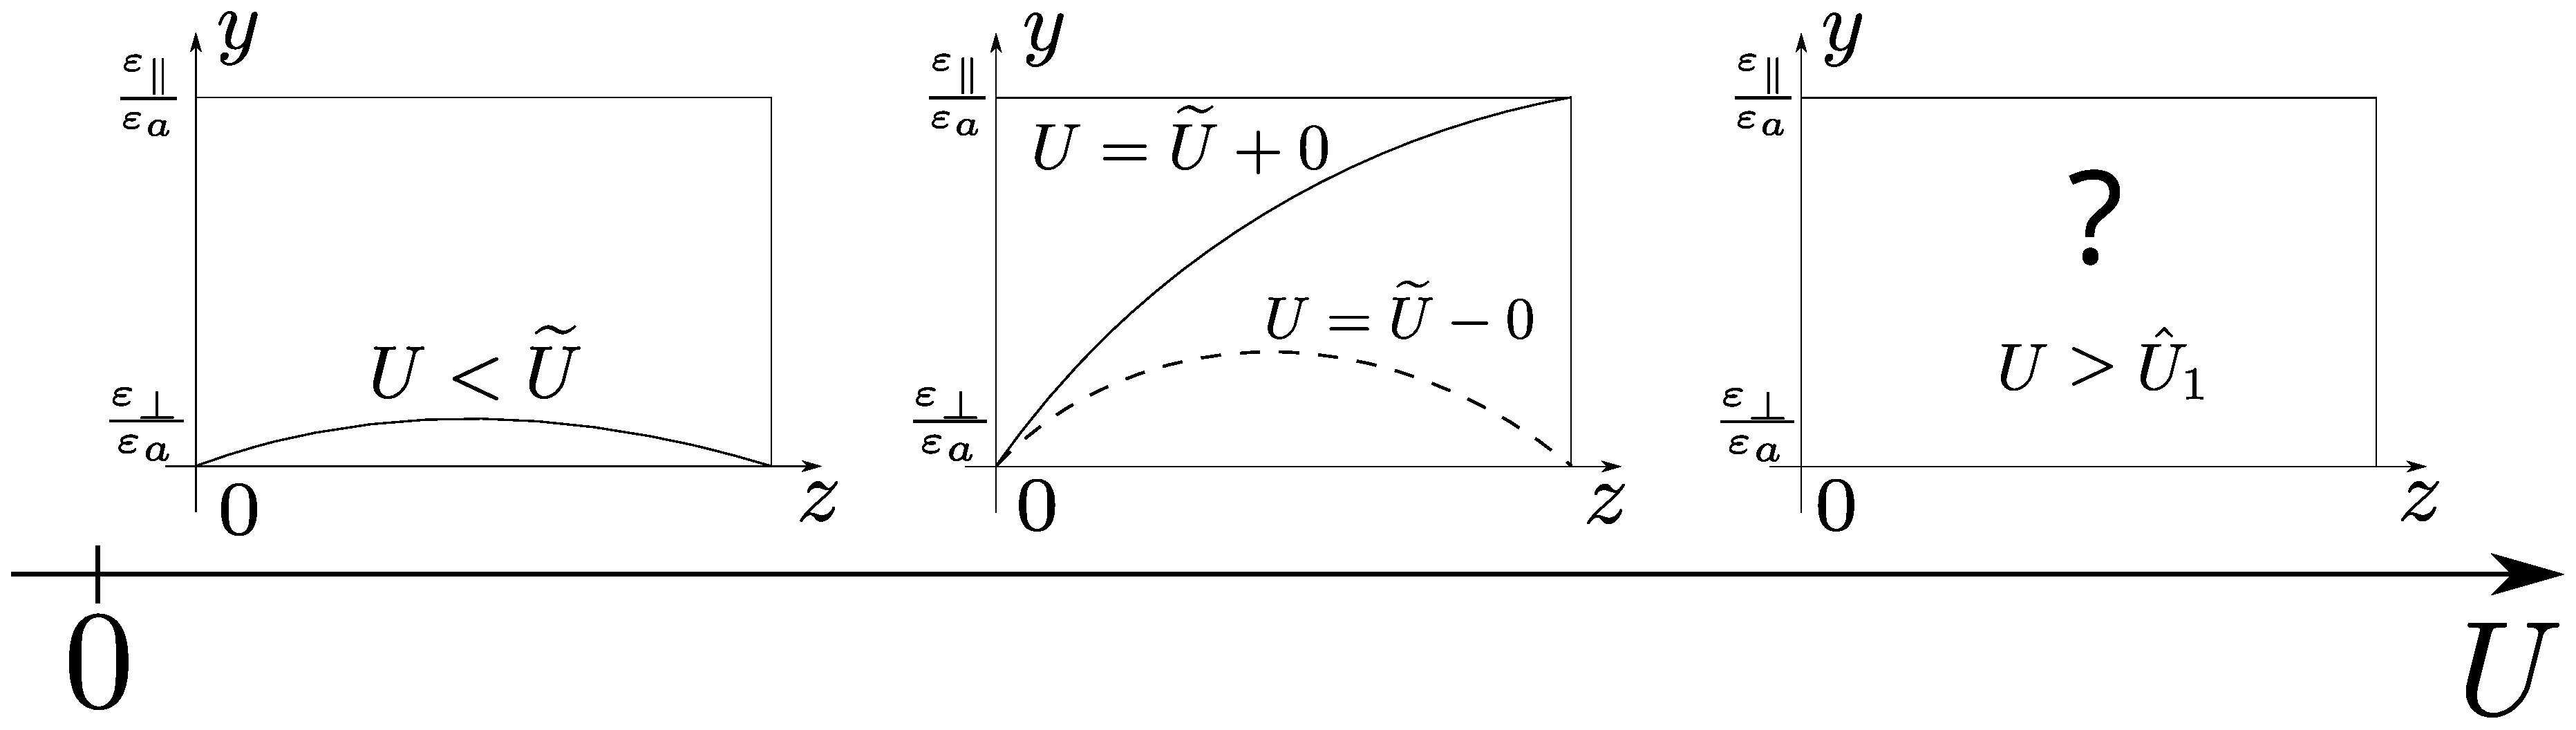
\includegraphics[width=\textwidth]{ch5_scheme_nonsaturated_part_3.eps}
		\caption{Схематическое изображение трансформации профилей $y(z)$ с ростом приложенного напряжения $U$ в случае ``слабого'' сцепления, задаваемого неравенством~\eqref{eq:ch5_case_2_ineqs_5_c}.}\label{fig:ch5_scheme_nonsaturated_part_3}
	\end{figure}
	Здесь симметричный параболический профиль остаётся равновесным, пока напряжение $U$ не превысит значения $\tilde{U}$, после чего равновесным становится параболический профиль с разными значениями на границах, задаваемый уравнением~\eqref{eq:ch5_asymmetric_parabolic_profile}.
	В свою очередь, асимметричный профиль без участков насыщения остаётся равновесным до достижения следующего порогового напряжения, $\hat{U}_1$, после чего равновесным будет уже профиль с участками насыщения.
	В данном случае оказалось неупомянутым напряжение $\hat{U}'$, так как симметричный профиль теряет устойчивость на правой границе ещё до того, как его вершина коснётся границы $y = \ve_\|/\ve_a$.
\end{itemize}

\section{Решения с участком насыщения}

Рассмотрим решения с единственным участком насыщения.
Расчёт равновесных профилей при помощи прямой минимизации свободной энергии проказал, что при $\ve_a, U > 0$ возникают профили только трёх типов.
Они схематически изображены на Рис.~\ref{fig:ch5_profiles_saturated}.
\begin{figure}
	\begin{minipage}{0.32\textwidth}
		\centering
		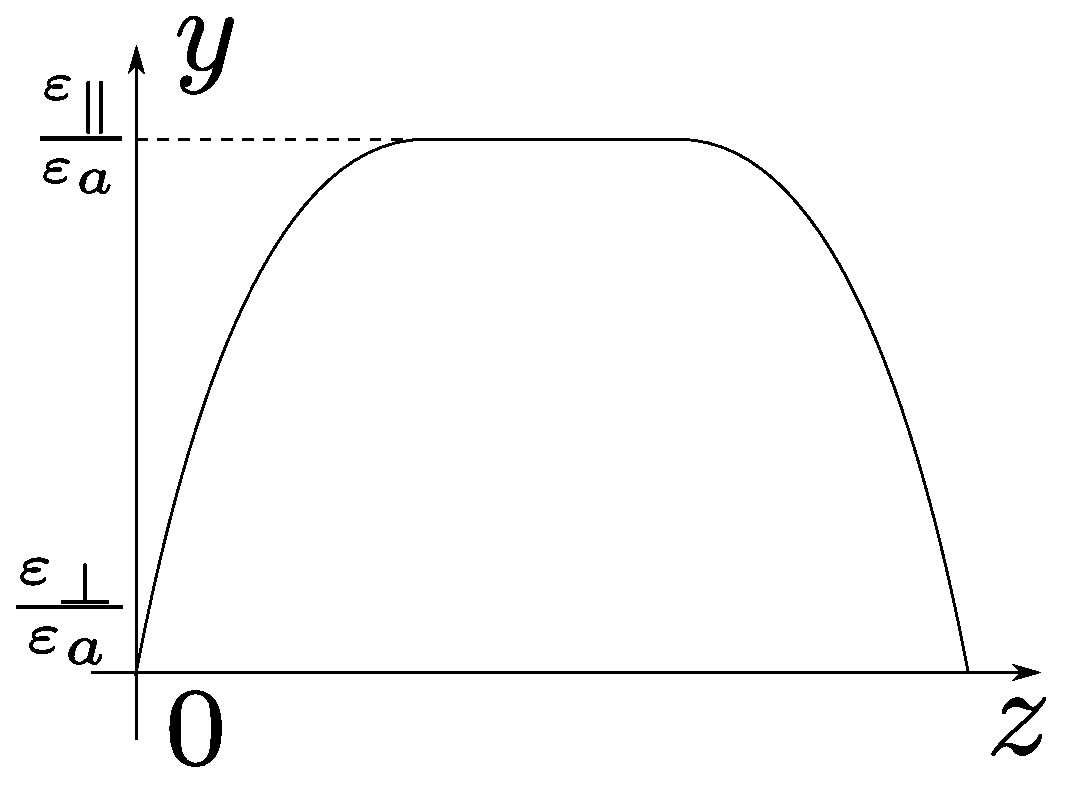
\includegraphics[width=\textwidth]{ch5_profiles_saturated_a.eps}
		{А}
	\end{minipage}
	\hfill
	\begin{minipage}{0.32\textwidth}
		\centering
		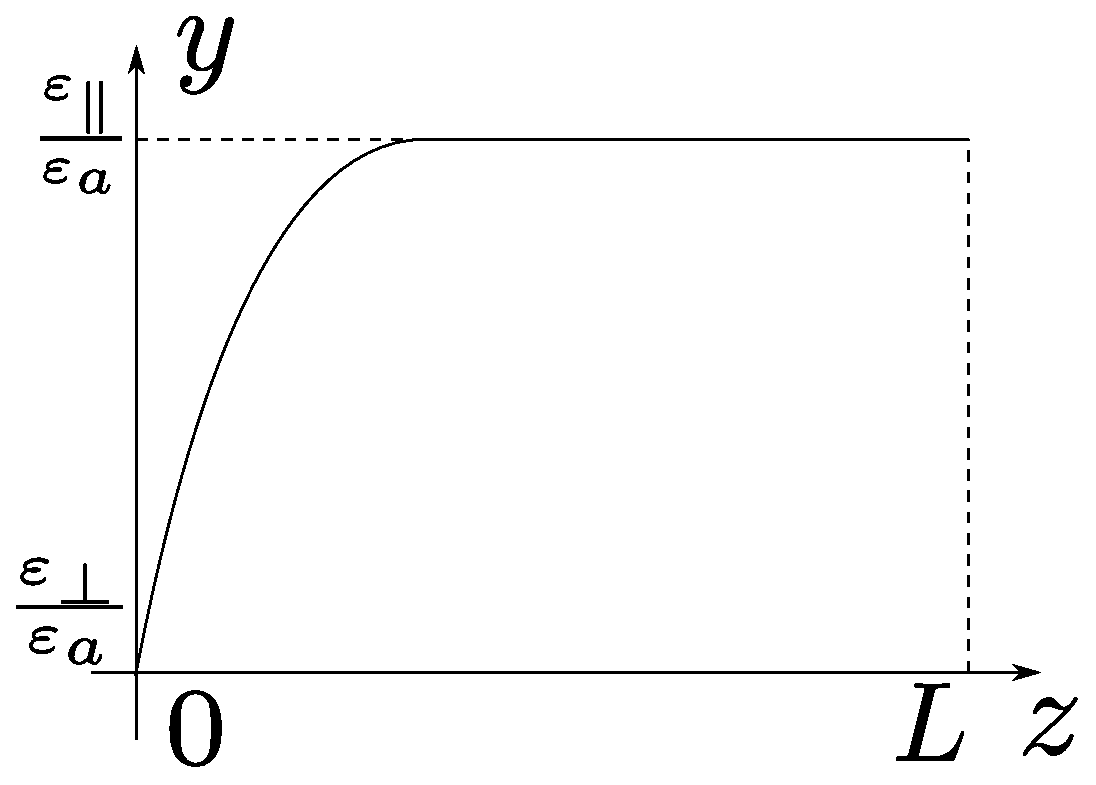
\includegraphics[width=\textwidth]{ch5_profiles_saturated_b.eps}
		{Б}
	\end{minipage}
	\hfill
	\begin{minipage}{0.32\textwidth}
		\centering
		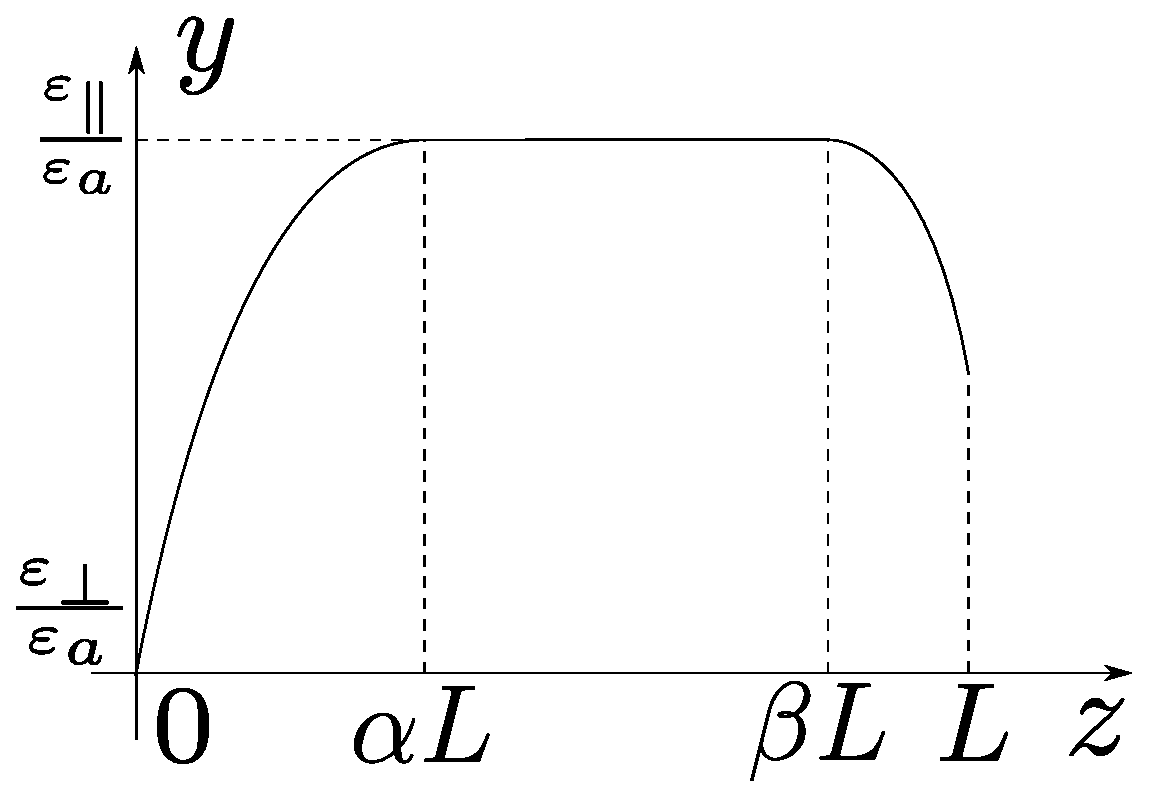
\includegraphics[width=\textwidth]{ch5_profiles_saturated_c.eps}
		{В}
	\end{minipage}
	\vspace{0.5cm}
	\caption{Схематическое изображение различных видов профилей с участками насыщения, полученных при помощи численной минимизации свободной энергии.}
	\label{fig:ch5_profiles_saturated}
\end{figure}
Перед тем, как мы начнём получать их уравнения, отметим следующую особенность: в данном случае искомая функция $y(z)$ состоит из нескольких частей.
При этом на каждую точку сшивания $z_0$ добавляется ещё по два условия: на функцию, $y(z_0 - 0) = y(z_0 + 0)$, и на производную, $y'(z_0 - 0) = y'(z_0 + 0)$.

\paragraph{Случай А. Симметричный профиль с участком насыщения.}
Будем искать решение следующего вида:
\begin{equation}
	y(z) = 
	\begin{cases}
		y_1(z),\quad z\in [0,\,\alpha L],\\
		\frac{\ve_\|}{\ve_a},\quad z\in (\alpha L,\, \beta L),\\
		y_3(z),\quad z\in [\beta L,\,L].
	\end{cases}
\end{equation}
Отметим, что и $y_1$, и $y_3$ должны решать одно и то же уравнение~\eqref{eq:parametric_EL}, а значит, обе они имеют вид~\eqref{eq:parabolic_solution} с общим коэффициентом $a$ и отличаясь только коэффициентами $b$ и $c$ ($b_1$, $c_1$ и $b_3$ и $c_3$ соответственно).
Запишем ``геометрические'' условия на функцию $y_1(z)$:
\begin{subequations}\label{eq:ch5_saturated_case_a_system_1}
	\begin{empheq}[left = \empheqlbrace]{align}
		&y_1(z) = \frac{c_1}{4}(z + b_1)^2 - \frac{a^2}{c_1},\label{eq:ch5_saturated_case_a_system_1_1}\\
		&y_1(0) = \frac{\ve_\bot}{\ve_a},\label{eq:ch5_saturated_case_a_system_2}\\
		&y_1(\alpha L) = \frac{\ve_\|}{\ve_a},\label{eq:ch5_saturated_case_a_system_3}\\
		&y_1'(\alpha L) = 0.\label{eq:ch5_saturated_case_a_system_4}
	\end{empheq}
\end{subequations}
Нетрудно видеть, что требование сшивания производных может быть выполнено тогда и только тогда, когда вершина параболы $y_1(z)$ находится в точке с координатами $(\alpha L,\, \ve_\|/\ve_a)$, а значит, $b_1 = -\alpha L$.
Подстановка~\eqref{eq:ch5_saturated_case_a_system_1} в~\eqref{eq:ch5_saturated_case_a_system_2} и~\eqref{eq:ch5_saturated_case_a_system_3} приводит к следующему виду $y_1(z)$:
\begin{equation}\label{eq:ch5_saturated_case_a_eq_3}
	y_1(z) = -\left( \frac{z}{\alpha L} - 1 \right)^2 + \frac{\ve_\|}{\ve_a}.
\end{equation}
Аналогичные рассуждения можно провести и для $y_3(z)$.
Отметим, что условия $y_1(0) = y_3(L)$ и $y_1(\alpha L) = y_3(\beta L)$ приводят к тому, что параболы $y_1(z)$ и $y_3(z)$ оказываются симметричными относительно $z = L/2$.
Это означает, в частности, что $\alpha = 1 - \beta$.
Таким образом, для $y_3(z)$ имеем:
\begin{equation}
y_3(z) = -\left( \frac{z}{\alpha L} - \frac{1}{\alpha} + 1 \right)^2 + \frac{\ve_\|}{\ve_a}.
\end{equation}
Кроме того, из этих же условий можно получить следующе выражение для $a$:
\begin{equation}\label{eq:ch5_saturated_case_a_eq_1}
	a = -\frac{2\varkappa}{\alpha L}.
\end{equation}
Для того, чтобы определить значение параметра $\alpha$, следует подставить полученную зависимость $y(z)$ в условие самосогласования~\eqref{eq:parameter_a}:
\begin{equation}\label{eq:ch5_saturated_case_a_eq_2}
	a\frac{(1 - 2\alpha)L}{2\varkappa^2} = \ln\left( \gamma \frac{\varkappa + 1}{\varkappa - 1} \right).
\end{equation}
Подставляя~\eqref{eq:ch5_saturated_case_a_eq_1} в~\eqref{eq:ch5_saturated_case_a_eq_2}, можно получить окончательное выражение для $1/\alpha$:
\begin{equation}
	\frac{1}{\alpha} = 2 - \varkappa\ln\left( \gamma\frac{\varkappa + 1}{\varkappa - 1} \right).
\end{equation}
Учитывая, что $\alpha$ ограниченa:
\begin{equation}
	0 < \alpha \leq \frac{1}{2},
\end{equation}
можно заметить, что в данном случае существует ограничение на $\gamma$:
\begin{equation}
	\gamma < \frac{\varkappa - 1}{\varkappa + 1}.
\end{equation}
Это эквивалентно условию $U > \hat{U}'$, где $\hat{U}'$ -- найденное в предыдущей части напряжение, при котором симметричный параболический профиль касается верхней границы (см. Рис.~\ref{fig:ch5_scheme_nonsaturated_part_1}).

Остаётся проверить, что выполнены граничные условия~\eqref{eq:ch5_parabolic_system_6} и~\eqref{eq:ch5_parabolic_system_7}.
Подстановка $y_1(z)$ в первое из них даёт
\begin{equation}
	g_1(\varkappa - 1)(\varkappa + 1) > \frac{2}{\alpha L}(1 - \varkappa),
\end{equation}
что верно всегда, поскольку $\varkappa > 1$.
Подстановка $y_3(z)$ во второе условие приводит к неравенству
\begin{equation}
	g_2 L > \frac{2}{\alpha(\varkappa - 1)}.
\end{equation}
Его можно интерпретировать следующим образом: так как $\alpha = \alpha(U)$, причём с ростом напряжения $\alpha$ монотонно уменьшается, то будет существовать некоторое критическое значение напряжения $\tilde{U}'$, при котором неравенство обратится в равенство, и при превышении которого исследуемый профиль перестанет быть равновесным.
Можно выписать явное выражение для этого порогового напряжения:
\begin{equation}
	\tilde{U}' = \hat{U}' + \frac{8\pi\bar{e}}{\ve_a}\left( \frac{g_2 L}{2}\cdot\frac{\varkappa - 1}{\varkappa} - \frac{2}{\varkappa} \right)
\end{equation}

Таким образом, симметричный профиль с участком насыщения является равновесным, когда выполнены два условия на напряжение, $\hat{U}' < U < \tilde{U}'$, причём указанный интервал напряжений непустой тогда и только тогда, когда $g_2L > 4/(\varkappa - 1)$.

\todo{Может, стоит привести итоговый вид функции $y(z)$ в виде кусочно-заданной функции?}

\paragraph{Асимметричный профиль с насыщеной правой границей.}
Рассмотрим профиль, схематически изображённый на Рис.~\ref{fig:ch5_profiles_saturated}\,Б.
Будем искать решение вида
\begin{equation}\label{eq:ch5_saturated_case_b_start}
y(z) = 
\begin{cases}
y_1(z),\quad z\in [0,\,\alpha L],\\
\frac{\ve_\|}{\ve_a},\quad z\in (\alpha L,\, L].
\end{cases}
\end{equation}
В данном случае необходимо найти единственную функцию $y_1(z)$, удовлетворяющую тем же условиям, что и одноимённая функция, найденная выше (система уравнений~\eqref{eq:ch5_saturated_case_a_system_1}); эти условия приводят к виду $y_1(z)$, повторяющему формулу~\eqref{eq:ch5_saturated_case_a_eq_3}:
\begin{equation}\label{eq:ch5_saturated_case_b_eq_1}
	y_1(z) = -\left( \frac{z}{\alpha L} - 1 \right)^2 + \frac{\ve_\|}{\ve_a}.
\end{equation}
Опять же, из этих условий можно получить выражение для $a$:
\begin{equation}\label{eq:ch5_saturated_case_b_eq_2}
	a = -\frac{2\varkappa}{\alpha L}.
\end{equation}
Подставляя~\eqref{eq:ch5_saturated_case_b_eq_1} в условие самосогласования~\eqref{eq:parameter_a}, получаем ещё одно уравнение:
\begin{equation}\label{eq:ch5_saturated_case_b_eq_3}
	a\frac{(1 - \alpha)L}{2\varkappa^2} = \ln\left( \gamma \frac{\varkappa + 1}{\varkappa} \right).
\end{equation}
Совмещая~\eqref{eq:ch5_saturated_case_b_eq_2} и~\eqref{eq:ch5_saturated_case_b_eq_3}, получаем выражение для $\alpha$:
\begin{equation}\label{eq:ch5_saturated_case_b_eq_4}
	\alpha = \left( 1 - \varkappa\ln\left( \gamma \frac{\varkappa + 1}{\varkappa} \right)\right)^{-1}.
\end{equation}
В данном случае мы также имеем ограничение на $\alpha$:
\begin{equation}
	0 < \alpha \leq 1.
\end{equation}
Видно, что это условие выполнено при $U > \hat{U}_1$, где $\hat{U}_1$ определено выражением~\eqref{eq:ch5_case_2_ineqs_5_c}.

Наконец, проверим, когда выполняется условия на границах.
подстановка $y_1(z)$ в~\eqref{eq:ch5_parabolic_system_6} приводит к тому же выражению, что было получено при рассмотрении предыдущего случая, а значит, и вывод совпадает: условие на границе $z = 0$ выполнено всегда.
Далее, подставляя~\eqref{eq:ch5_saturated_case_b_start} в~\eqref{eq:ch5_parabolic_system_7}, получаем неравенство:
\begin{equation}\label{eq:ch5_saturated_case_b_eq_5}
	g_2 \varkappa^2 + a \leq 0,
\end{equation}
откуда, с учётом~\eqref{eq:ch5_saturated_case_b_eq_2} и~\eqref{eq:ch5_saturated_case_b_eq_4}, можно получить, что существует критическое напряжение $\hat{U}_2$ такое, что при $U > \hat{U}_2$ условие~\eqref{eq:ch5_saturated_case_b_eq_4} будет выполнено.
Приведём явный вид выражения для $\hat{U}_2$:
\todo{
\begin{equation}
	\hat{U}_2 = \hat{U}_1 + \frac{8\pi\bar{e}}{\ve_a}\cdot\frac{1}{\varkappa}\left( \frac{g_2 L}{2} - 1\right)
\end{equation}
}
Отметим, что при рассмотрении данного вида профилей не возникает условия на $g_2 L$, а значит, такой профиль возникает в системе с любым значением $g_2 L$ при достаточно большом напряжении ($U > \hat{U}_2$).


\paragraph{Асимметричный профиль с ненасыщеной правой границей.}
Рассмотрим профиль, схематически изображённый на Рис.~\ref{fig:ch5_profiles_saturated}\,В.
Выпишем все уравнения, которым должно удовлетворять решение:
\begin{subequations}\label{eq:ch5_saturated_case_c_system_1}
	\begin{empheq}[left = \empheqlbrace]{align}
		&y(0) = \frac{\ve_\bot}{\ve_a},\label{eq:ch5_saturated_case_c_system_1_1}\\
		&y(\alpha L) = \frac{\ve_\|}{\ve_a},\\
		&y(\beta L) = \frac{\ve_\|}{\ve_a},\\
		&y'(\alpha L) = 0,\\
		&y'(\beta L) = 0,\label{eq:ch5_saturated_case_c_system_1_5}\\
		&aJ^{-1} = J_1 - \frac{U}{4\pi\bar{e}},\label{eq:ch5_saturated_case_c_system_1_6}\\
		&y'(L) + a + g_2y(L) = 0,\label{eq:ch5_saturated_case_c_system_1_7}
	\end{empheq}
\end{subequations}
и все неравенства:
\begin{subequations}\label{eq:ch5_saturated_case_c_system_2}
	\begin{empheq}[left = \empheqlbrace]{align}
		&0 < \alpha < \beta < L,\\
		&y(L) \geq \frac{\ve_\bot}{\ve_a},\label{eq:ch5_saturated_case_c_system_2_2}\\
		& -(y'(0) + a) + g_1 y(0) \geq 0.\label{eq:ch5_saturated_case_c_system_2_3}
	\end{empheq}
\end{subequations}
Решение будем искать в виде
\begin{equation}
	y(z) = 
	\begin{cases}
		\frac{c_1}{4}\left( z + b_1 \right)^2 - \frac{a^2}{c_1}, &z\in[0,\alpha L),\\
		\frac{\ve_\|}{\ve_a}, &z\in[\alpha L,\, \beta L],\\
		\frac{c_2}{4}\left( z + b_2 \right)^2, &z\in(\beta L,\, L].
	\end{cases}
\end{equation}
Учёт уравнений~\eqref{eq:ch5_saturated_case_c_system_1_1} - \eqref{eq:ch5_saturated_case_c_system_1_5} позваляет записать $y_1(z)$ и $y_3(z)$ в следующем виде:
\begin{align}\label{eq:ch5_saturated_case_c_y_cases}
	&y_1(z) = -\left( \frac{z}{\alpha L} - 1 \right)^2 + \frac{\ve_\|}{\ve_a}\\
	&y_3(z) = -\left( \frac{z}{\alpha L} - \frac{\beta}{\alpha} \right)^2 + \frac{\ve_\|}{\ve_a},\label{eq:ch5_saturated_case_c_eq_1}
\end{align}
Кроме того, остаётся справедливым равенство~\eqref{eq:ch5_saturated_case_b_eq_2}.
Отметим, что подстановка~\eqref{eq:ch5_saturated_case_c_eq_1} в~\eqref{eq:ch5_saturated_case_c_system_2_2} приводит к следующему неравенству:
\begin{equation}
	\alpha \geq 1 - \beta.
\end{equation}
Далее, как и в предыдущих случаях, условие на границе $z = 0$ (неравенство~\eqref{eq:ch5_saturated_case_c_system_2_3}) оказывается выполненным всегда.
Напротив, подставляя~\eqref{eq:ch5_saturated_case_c_eq_1} в условие на границе $z = L$ (уравнение~\eqref{eq:ch5_saturated_case_c_system_1_7}), получаем следующее равенство:
\begin{equation}\label{eq:ch5_saturated_case_c_eq_2}
	(1 - \beta) - \varkappa\alpha = -\frac{2}{g_2 L}.
\end{equation}
Наконец, подстановка~\eqref{eq:ch5_saturated_case_c_y_cases} в условие самосогласования~\eqref{eq:ch5_saturated_case_c_system_1_6} после несложных преобразований и учёта связи $\alpha$ и $\beta$~\eqref{eq:ch5_saturated_case_c_eq_2} приводит к уравнению следующего вида;
\begin{equation}\label{eq:ch5_k/x+ln_x}
	\frac{k}{x} + \ln x = A(U),
\end{equation}
где введены обозначения:
\begin{align}
	&x = \alpha,\\
	&k = \frac{1}{\varkappa}\left( \frac{2}{g_2 L} + 1 \right),\\
	&A(U) = \frac{\ve_a U}{8\pi\bar{e}} + \frac{1}{\hat{\gamma}_1} - \ln\left( \frac{g_2 L}{2}(\varkappa + 1) \right).
\end{align}
Уравнение~\eqref{eq:ch5_k/x+ln_x} решается численно, однако можно найти, когда это решение существует и удовлетворяет нашим требованиям.

Возможны два случая: $k > 1$ и $k < 1$.
Графики функции  $f(x) = \ln(x) + k/x$ для обоих случаев приведены на Рис.~\ref{fig:ch5_graph_solver_3}.
\begin{figure}
	\begin{minipage}{0.35\textwidth}
		\centering
		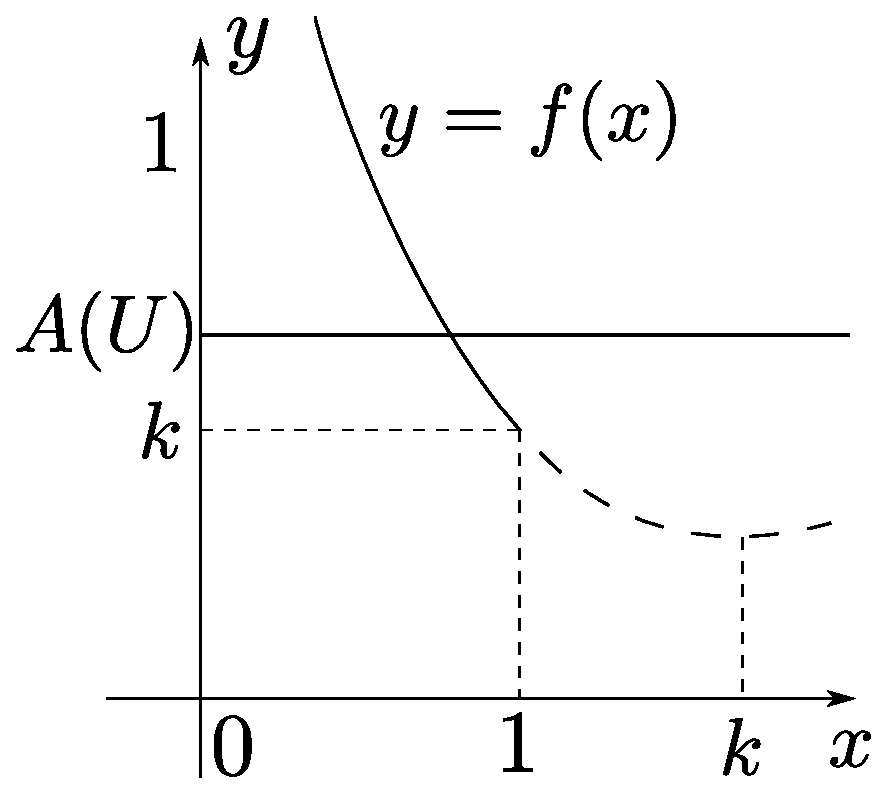
\includegraphics[width=\textwidth]{ch5_graph_solver_3a.eps}
		{А}
	\end{minipage}
	\hfill
	\begin{minipage}{0.52\textwidth}
		\centering
		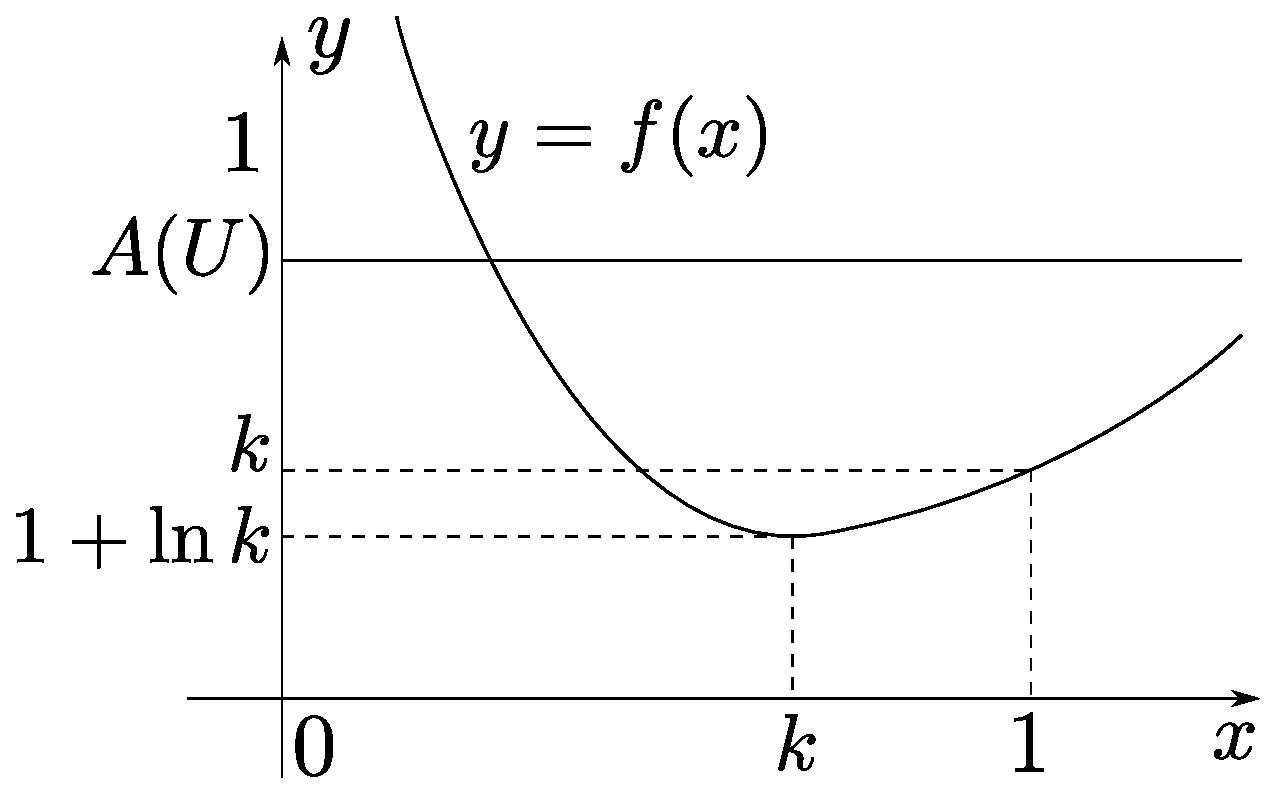
\includegraphics[width=\textwidth]{ch5_graph_solver_3b.eps}
		{Б}
	\end{minipage}
	\vspace{0.5cm}
	\caption{Графики функции $y = f(x)$ в случае $k > 1$ (А) и $k < 1$ (Б).}
	\label{fig:ch5_graph_solver_3}
\end{figure}
Нетрудно видеть, что выолняются следующие утверждения:
\begin{align}
	&A(0) < \ln{k} + 1, \quad k\in\left(\frac{1}{\varkappa},\, 1\right)\\
	&A(0) < k, \quad k > 1.
\end{align}
Отсюда следует, что при $U = 0$ решений у уравнения~\eqref{eq:ch5_k/x+ln_x} быть не может.
Однако с ростом $U$ горизонтальная прямая $y = A(U)$ начинает монотонно подниматься, и при некотором $U$ решение у уравнения~\eqref{eq:ch5_k/x+ln_x} появится.

Рассмотрим условия, которые наложены на решение:
\begin{subequations}
	\begin{empheq}[left = \empheqlbrace]{align}
		&\alpha \geq 1 - \beta,\\
		&\alpha < \beta,\\
		&1 - \beta \geq 0.
	\end{empheq}
\end{subequations}
С учётом связи~\eqref{eq:ch5_saturated_case_c_eq_2} их можно записать только для $\alpha$:
\begin{subequations}\label{eq:ch5_saturated_case_c_last_ineqs}
	\begin{empheq}[left = \empheqlbrace]{align}
		&\alpha \leq \frac{k\varkappa - 1}{\varkappa - 1},\\
		&\alpha < \frac{k\varkappa}{\varkappa + 1},\label{eq:ch5_saturated_case_c_last_ineqs_b}\\
		&\alpha > k - \frac{1}{\varkappa}.
	\end{empheq}
\end{subequations}
Заметим, что из неравенства~\eqref{eq:ch5_saturated_case_c_last_ineqs_b} следует, что искомая точка пересечения графика функции $y = f(x)$ и прямой $y = A(U)$, удовлетворяющая всем условиям, находится левее минимума функции$f(x)$ ($x = k$).
Таким образом, нужно смотреть лишь за пересечением $y = A(U)$ с левой ``ветвью'' $y = f(x)$.
Рис.~\ref{fig:ch5_graph_solver_4} иллюстрирует, какие неравенства из системы~\eqref{eq:ch5_saturated_case_c_last_ineqs} являются определяющими при различных значениях параметра $k$ (и, соответственно, $g_2 L$).
\begin{figure}[h]
	\centering
	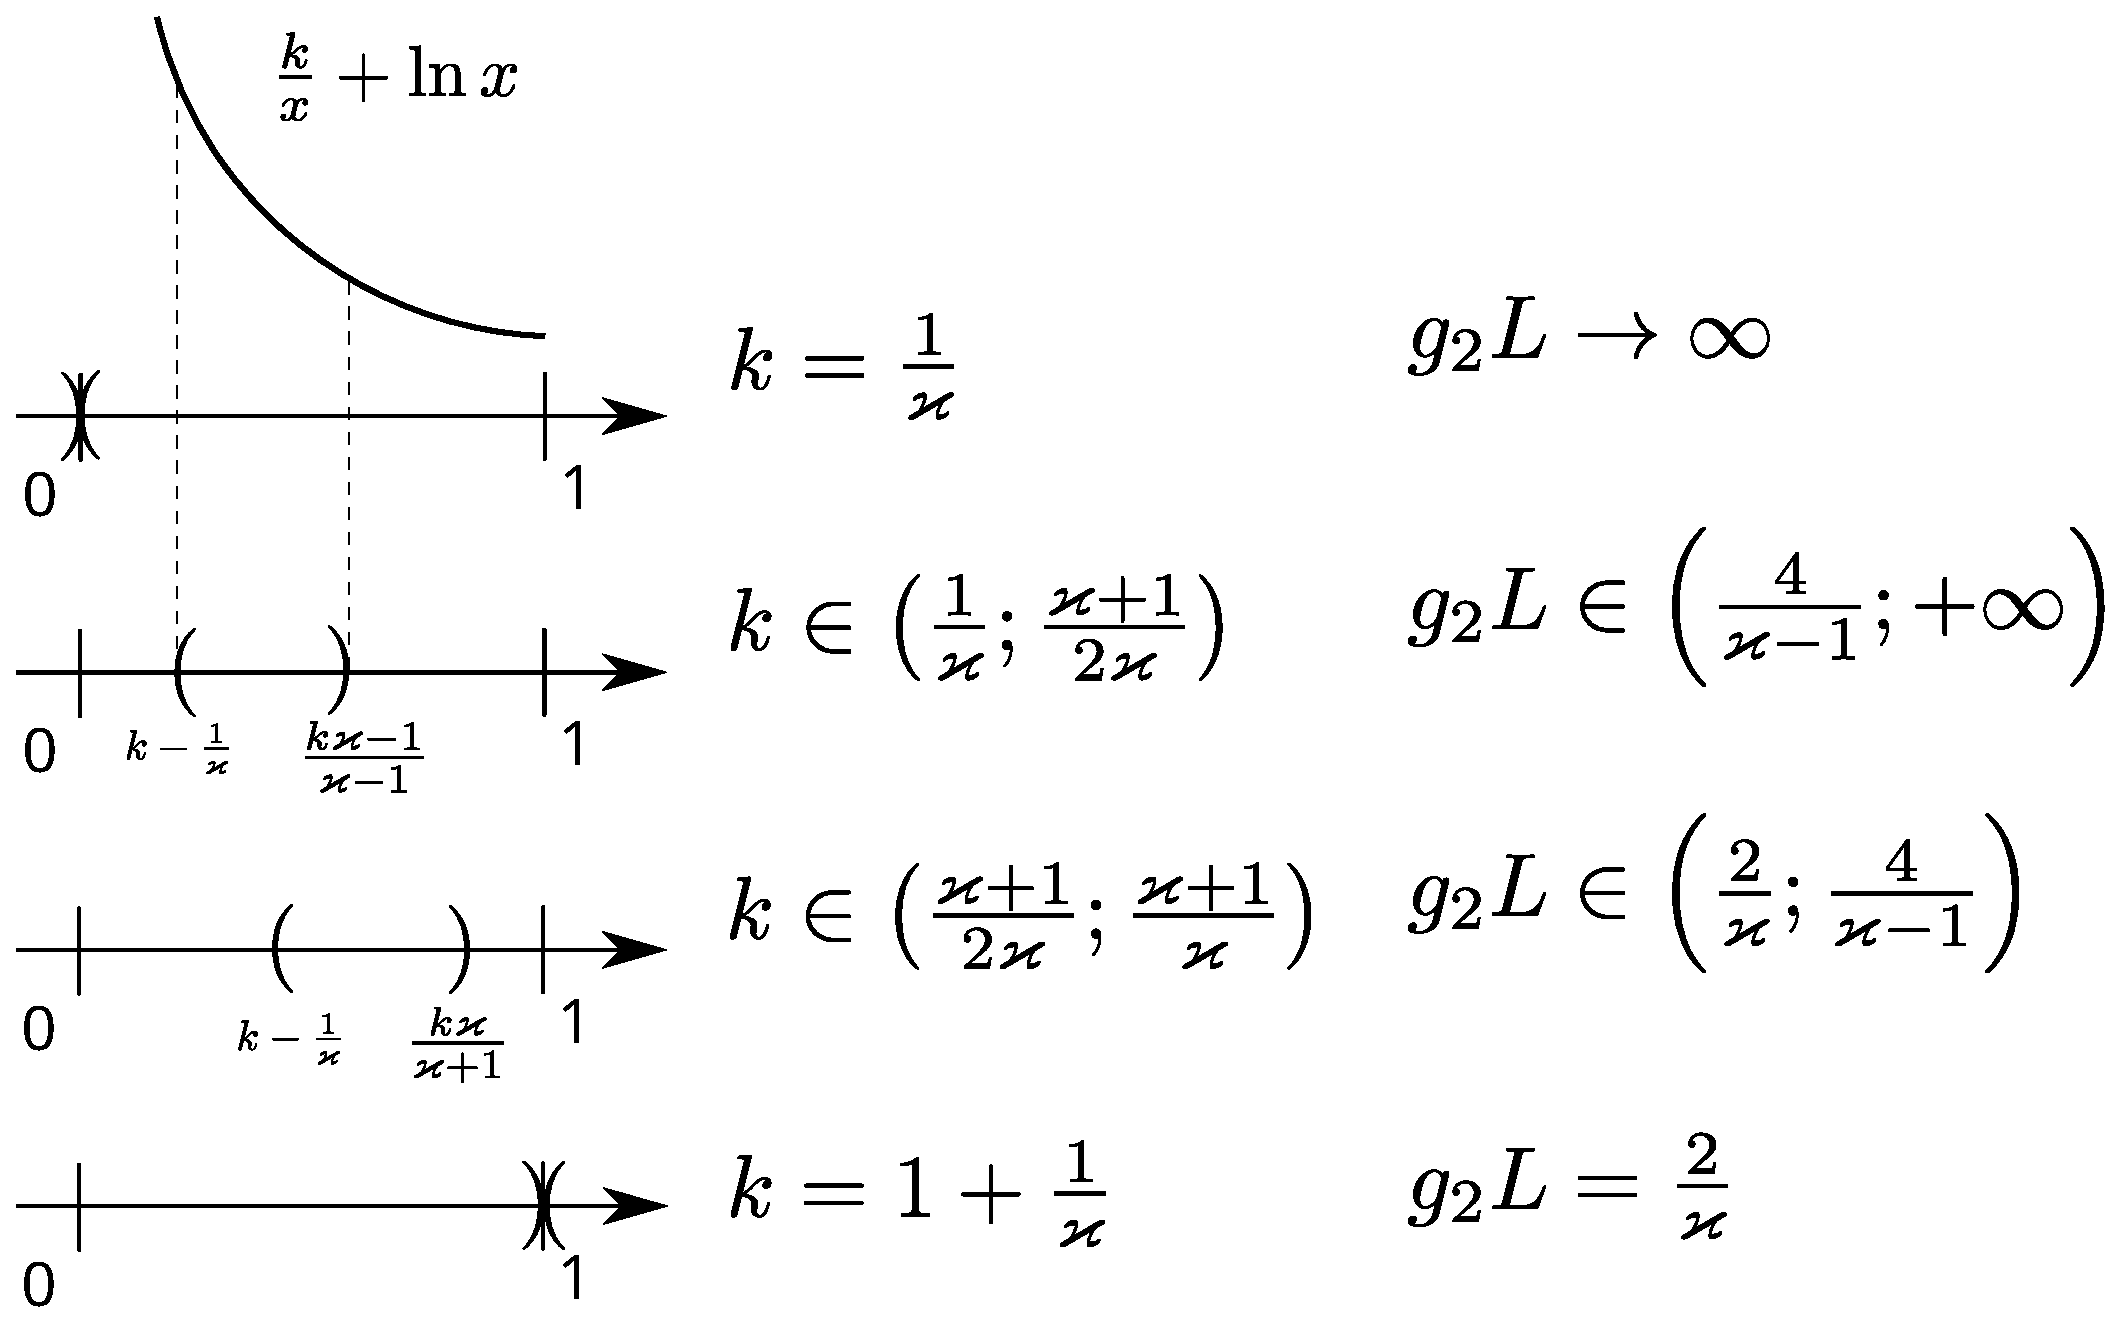
\includegraphics[width=0.8\textwidth]{Inequalities_k.eps}
	\caption{Графики функций $y = f_1(\gamma)$ и $y = f_2(\gamma)$. Цветом выделен участок на оси $\gamma$, соответствующий решению неравенства~\eqref{eq:ch5_case_2_ineq_2}.}\label{fig:ch5_graph_solver_4}
\end{figure}
Отметим, что отмеченные допустимые интервалы на Рис.~\ref{fig:ch5_graph_solver_4} являются интервалами для $\alpha$.
Чтобы найти соответствующие им интервалы напряжений, нужно найти проекцию соответствующего интервала на ось ординат (через график функции $y = f(x)$), а затем вычислить, в каких пределах должно меняться напряжение $U$, чтобы $A(U)$ находилась в обозначенных пределах.

На Рис.~\ref{Scheme} представлена полученная схема эволюции равновесного профиля в зависимости от значения параметра $g_2 L$. 
\begin{figure}[h]
	\centering
	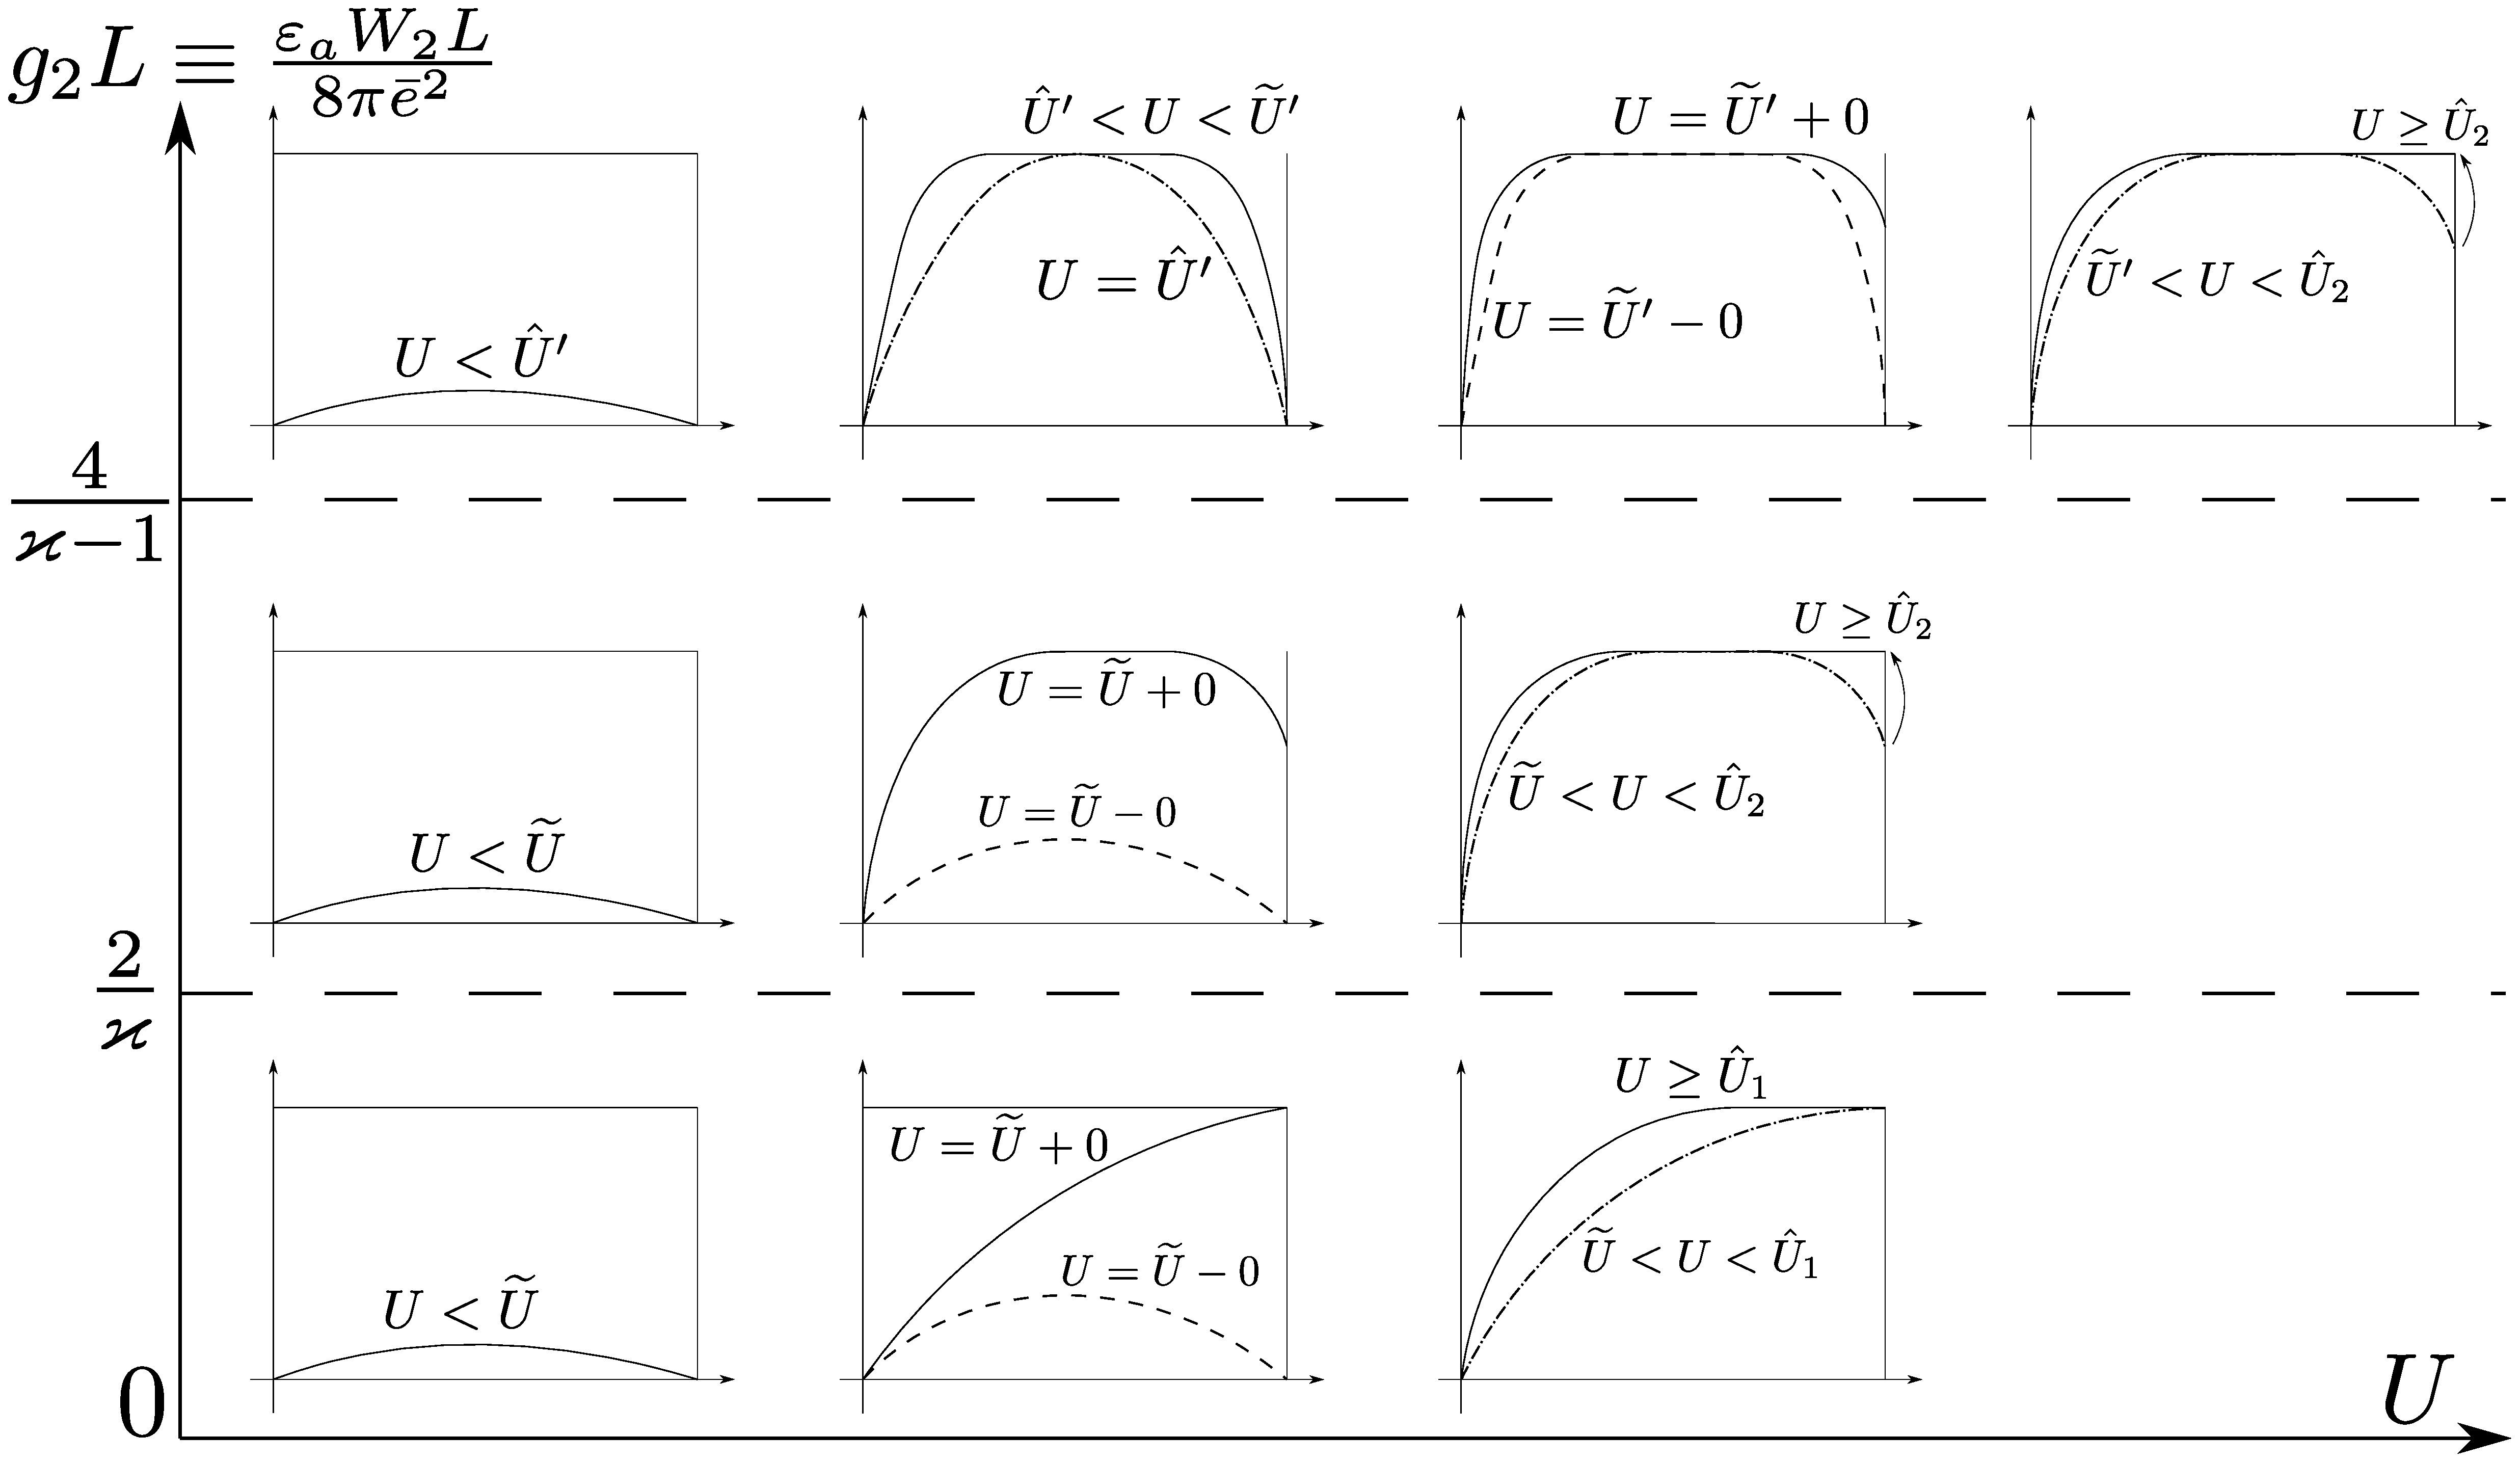
\includegraphics[width=\textwidth]{Scheme.eps}
	\caption{Схема переходов между профилями различных типов в зависимости от значения параметра $g_2 L$.}
	\label{Scheme}
\end{figure}

\section{Сравнение аналитических результатов с расчётными}
В заключение приведём сравнение профилей, рассчитанных при помощи полной модели свободной энергии (\todo{x.xx}) и профилей, полученных аналитически нна основе анализа сокращённой модели свободной энергии (\todo{y.yy}).

Методика поиска равновесной ориентационной структуры ЖК в ячейке путём численной минимизации функционала свободной энергии аналогична таковой, применённой в главе~\ref{ch:ch4}.
При этом был использован следующий набор параметров системы: $L = 0.006$~см, $\ve_\bot = 7.2$, $\ve_\|  = 16.2$, $\ve_a = 9$, $\bar{e} = 0.01$~Фр/см.
Было обнаружено, что, в зависимости от значения $g_2 L$, трансформация ориентационной структуры с изменением приложенного напряжения $U$ может происходить по трём различным сценариям, что соответствует результату, полученному аналитически.
На Рис.~\ref{ch5:fig1} показана трансформация ориентационной структуры при достаточно небольшой энергии сцепления с правой подложкой $W_\theta^{(2)}$, когда выполнено следующее неравенство:
\begin{equation}\label{ineq_g2L_1}
g_2 L < \frac{2}{\varkappa},
\end{equation}
где $\varkappa = \sqrt{\ve_\| /\ve_a}$.
\begin{figure}[h]
	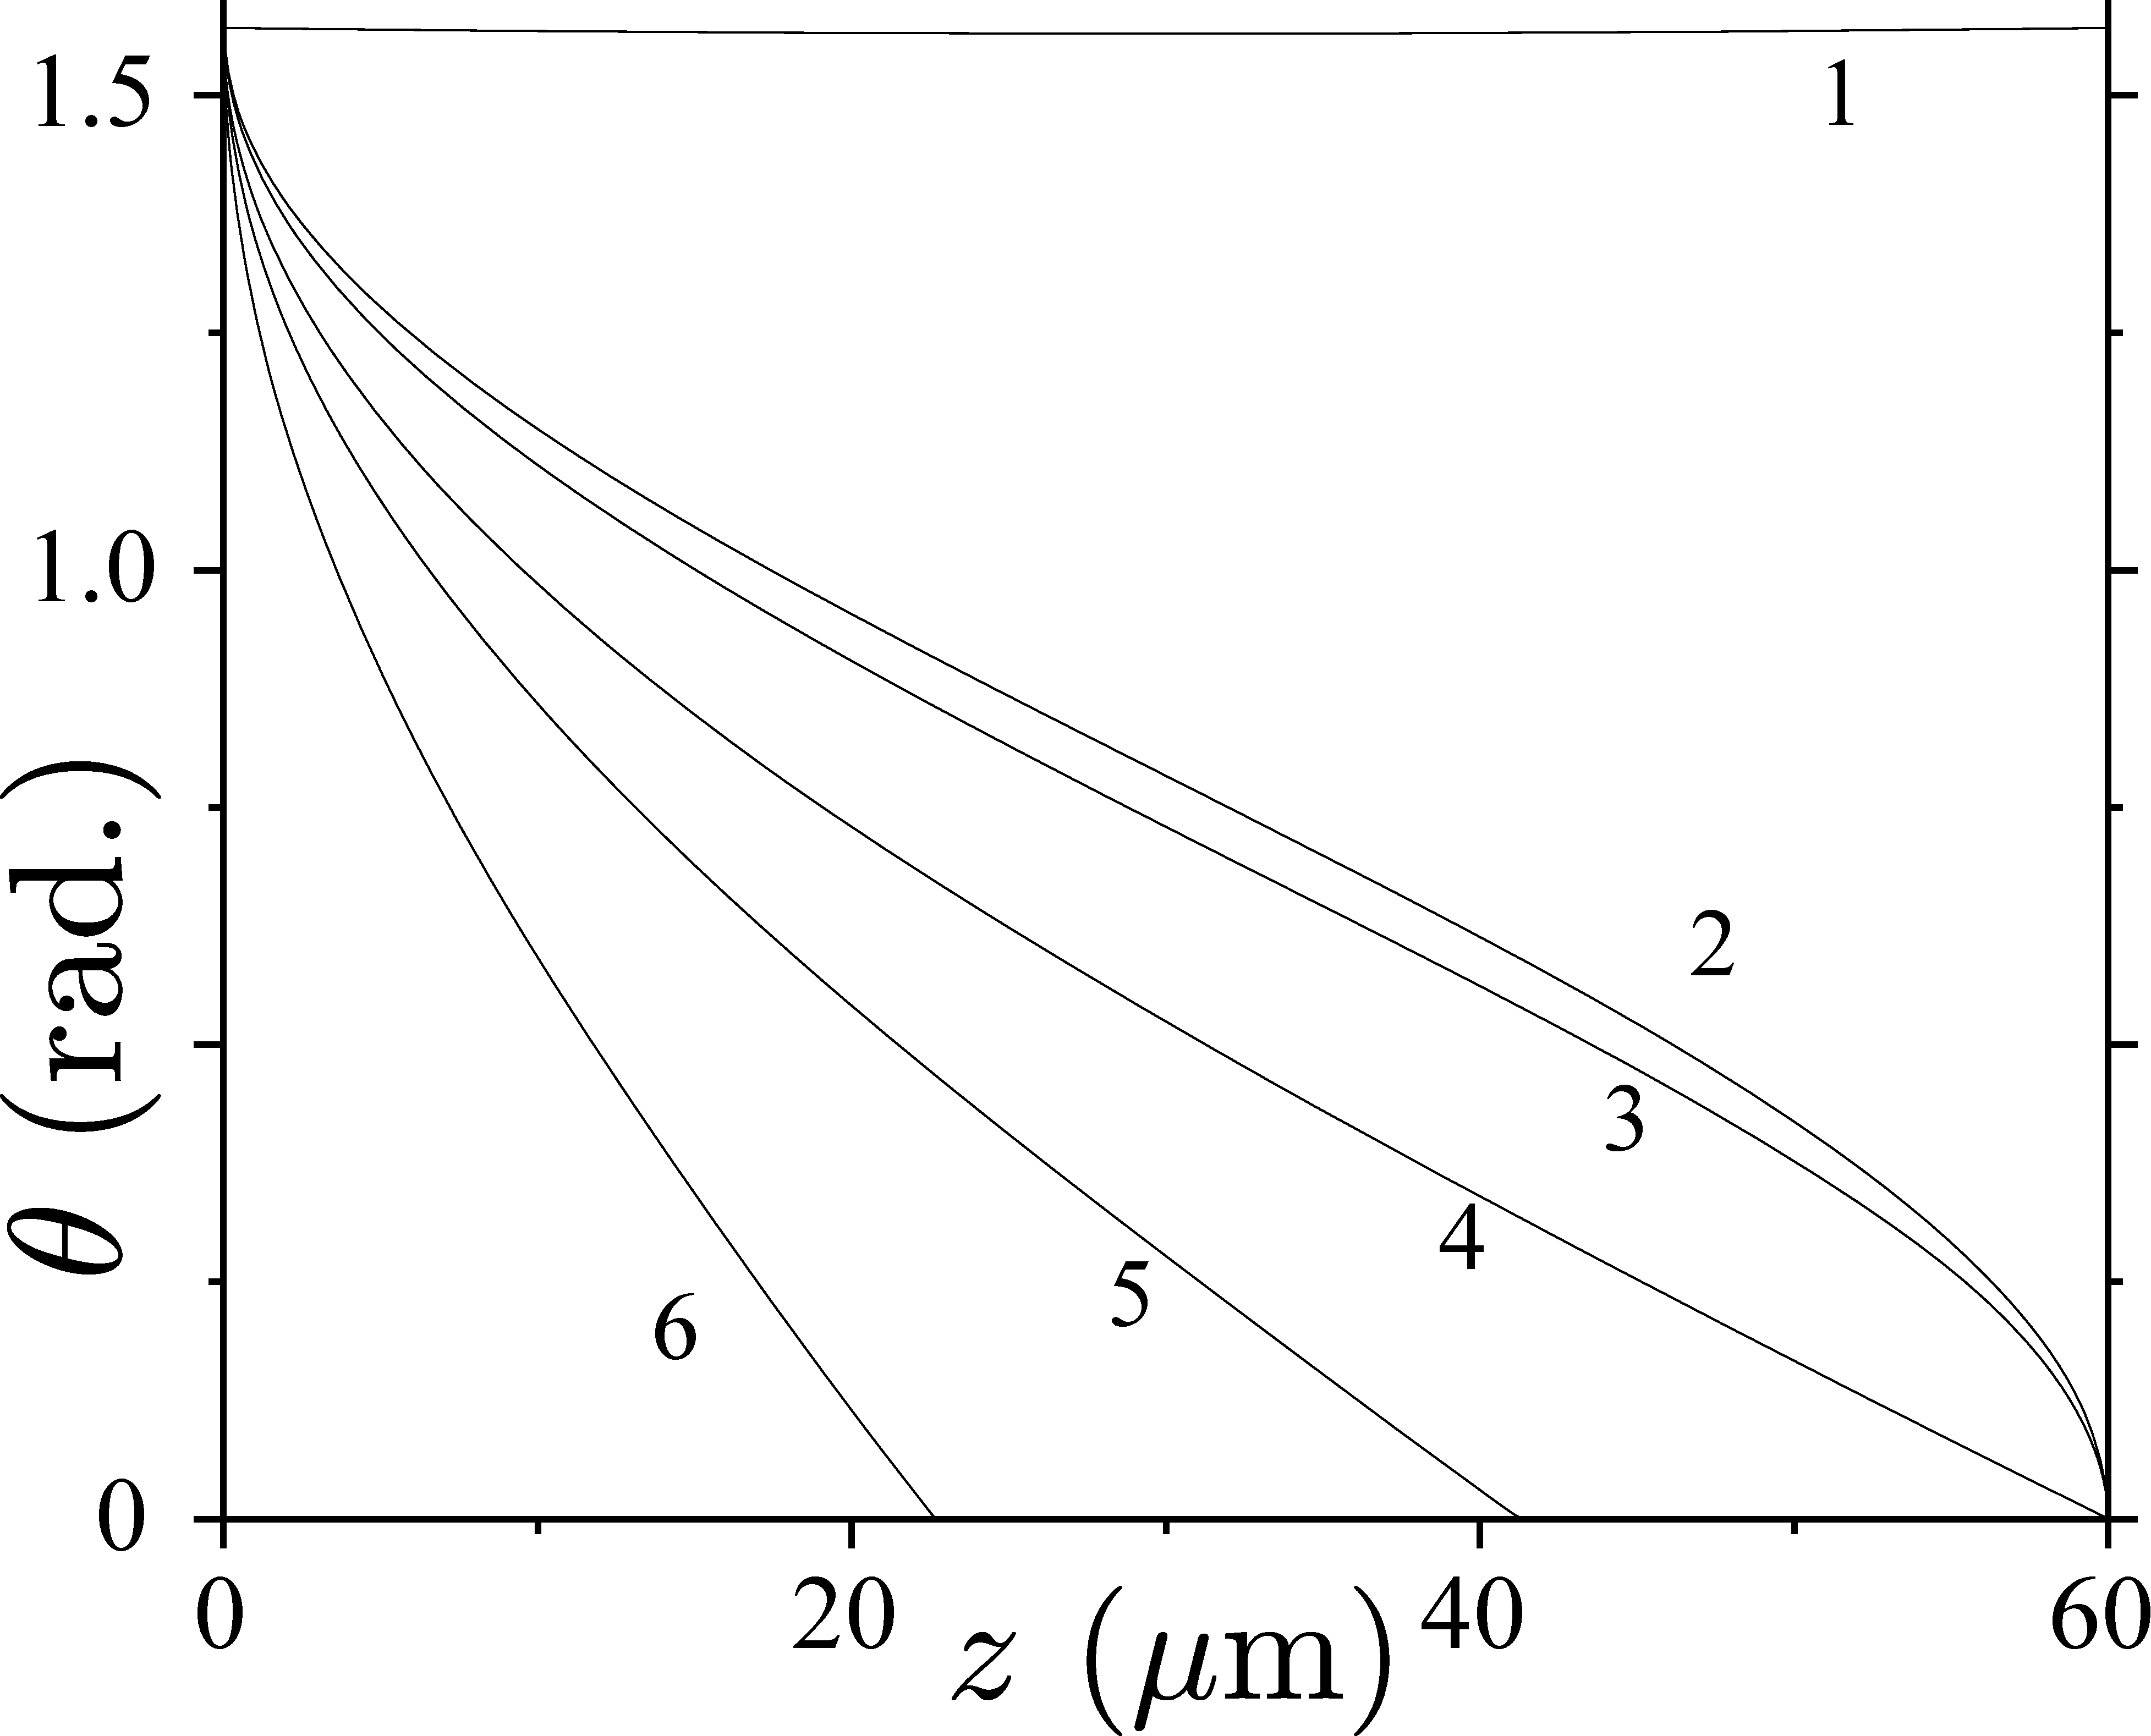
\includegraphics[width=17pc]{Fig1_theta_low_anchoring.eps}\hspace{2pc}%
	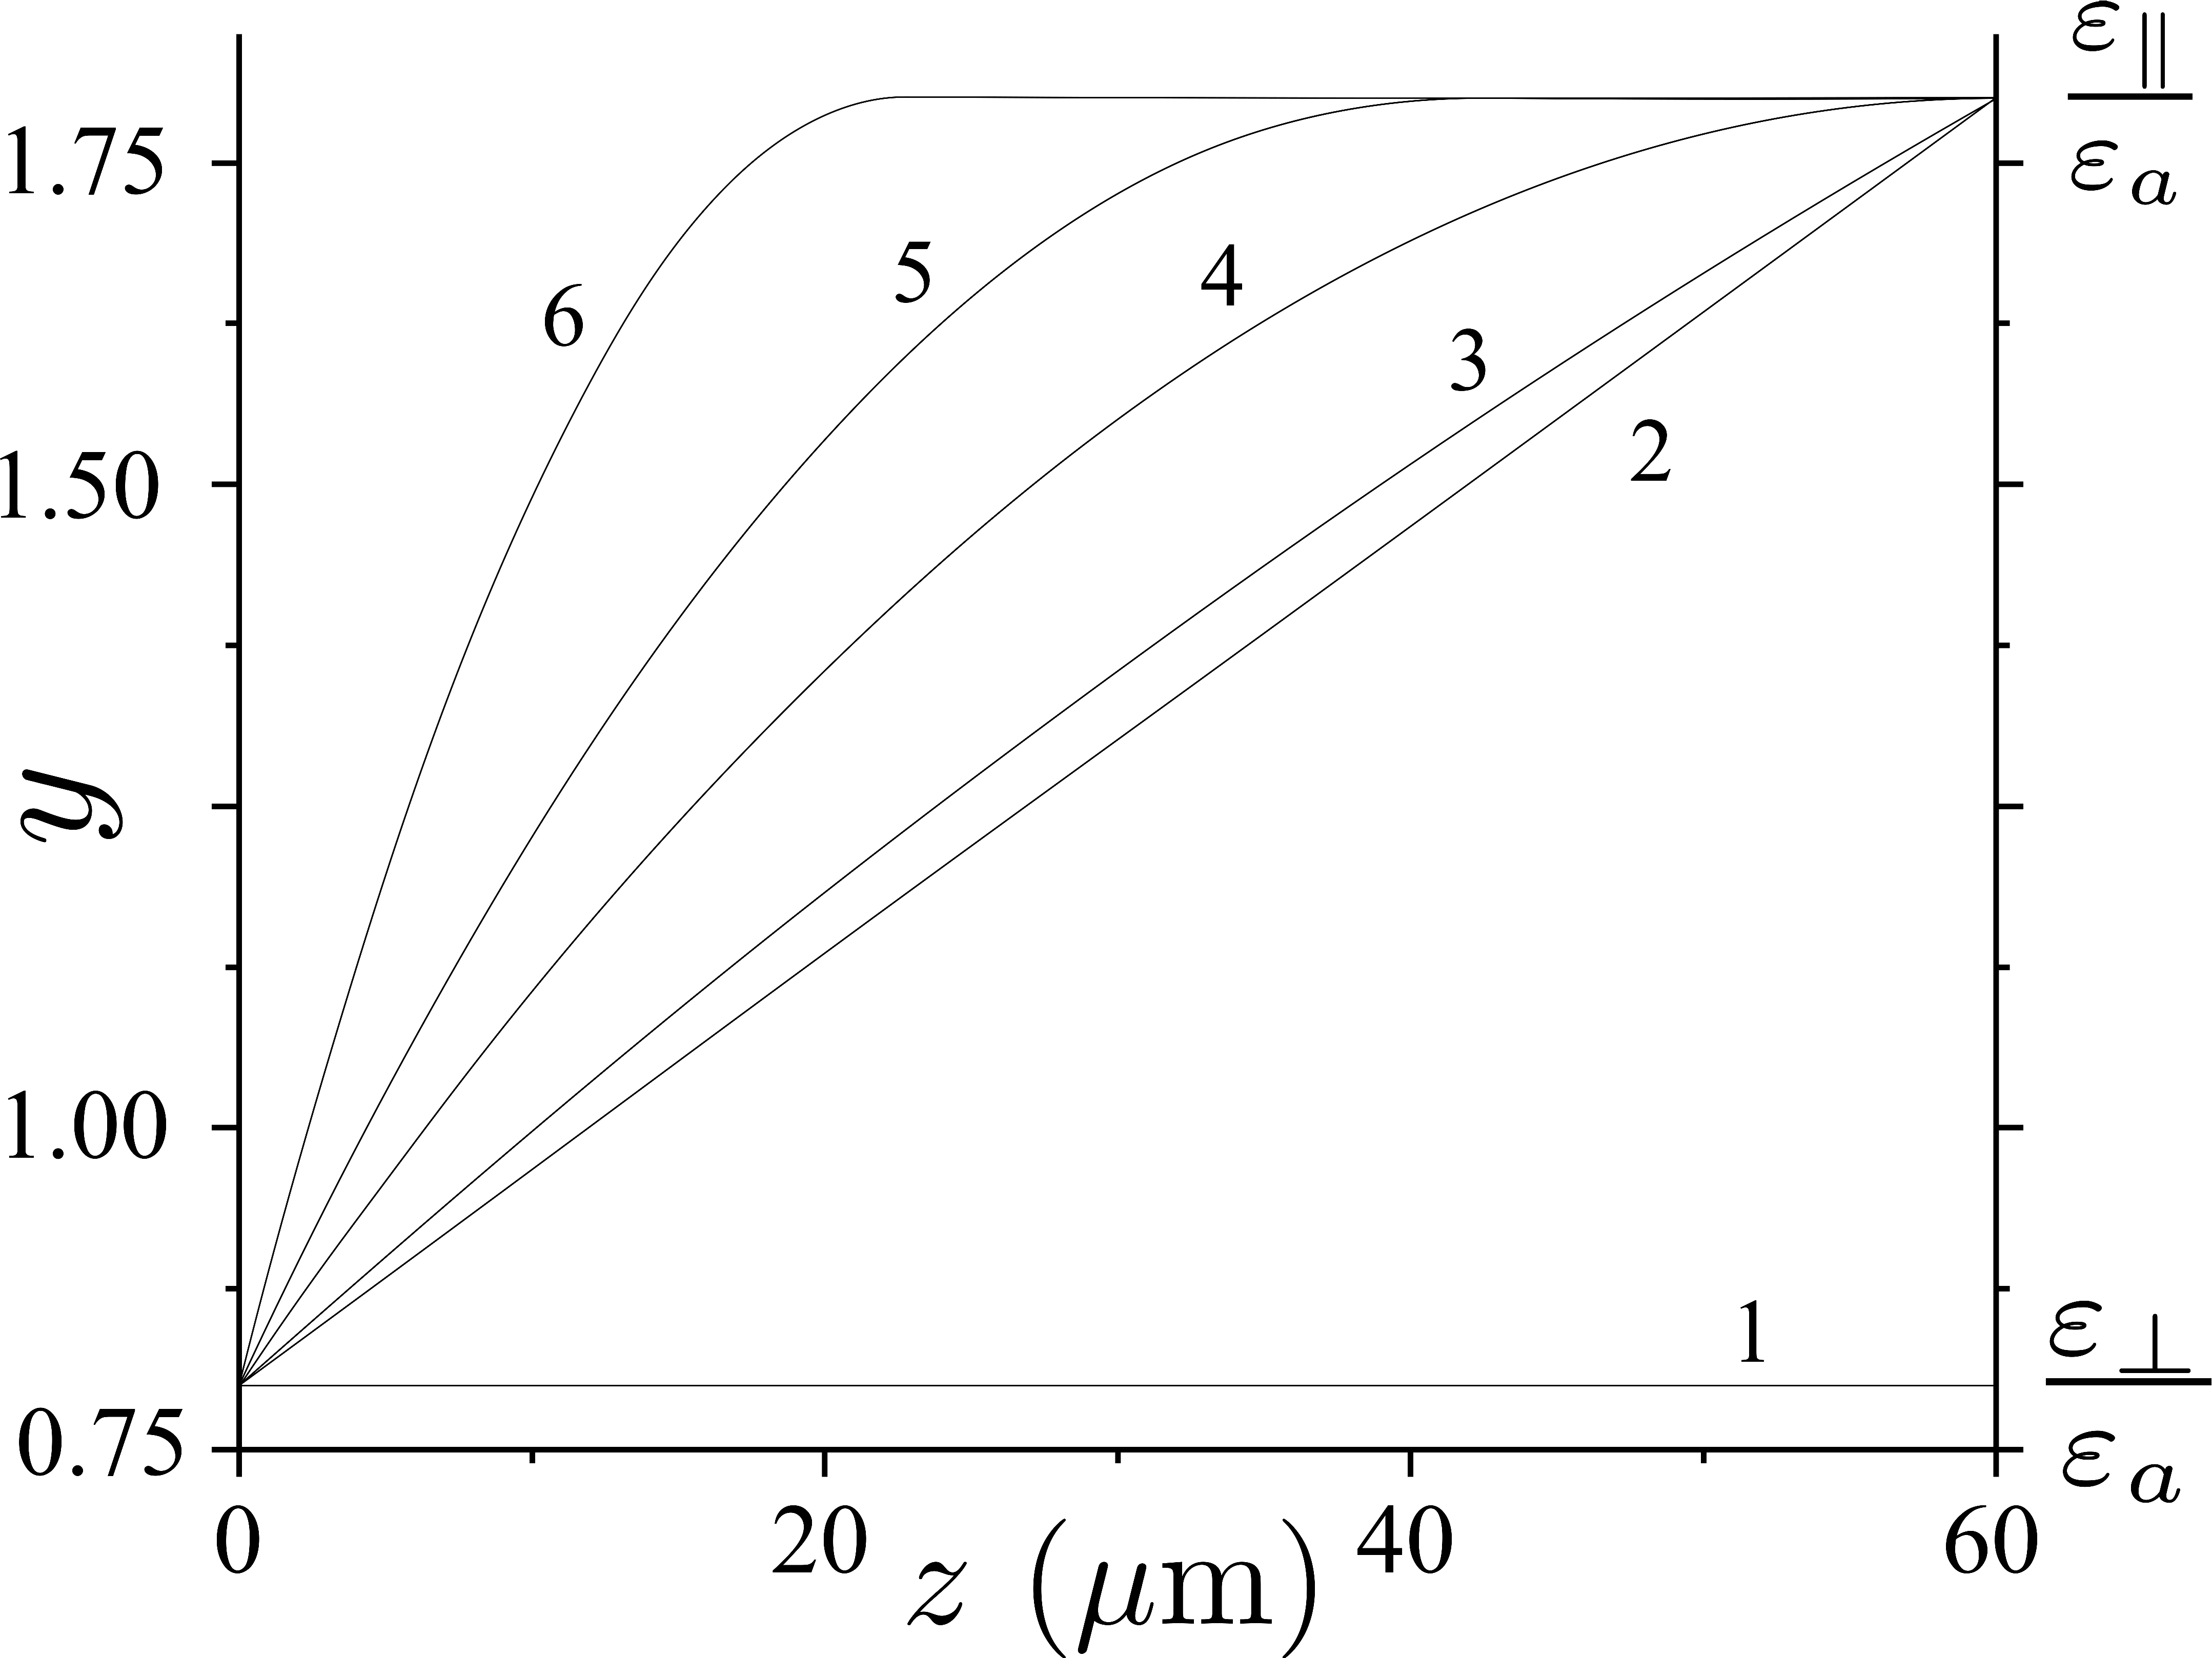
\includegraphics[width=18.8pc]{Fig1_y_low_anchoring.eps}
	\caption{Графики зависимостей $\theta(z)$ (слева) и $y(z)$ (справа), полученные в случае слабого сцепления с правой подложкой, когда выполнено неравенство~\eqref{ineq_g2L_1}.
		Модули сцепления с границами для каждого графика: $W_\theta^{(1)}=0.0025\ \text{эрг}/\text{см}^2$, $W_\theta^{(2)} = 5\times 10^{-4}\ \text{эрг}/\text{см}^2$
		Соответствие линий и приложенного напряжения: 1 -- $U = 0.04$~В, 2 -- $U = 0.05$~В, 3 -- $U = 1.5$~В, 4 -- $U = 4.67$~В, 5 -- $U = 7.5$~В, 6 -- $U = 15$~В.}\label{ch5:fig1}
\end{figure}
Отметим, что кривая $1$ сответствует области малых напряжений $U$, и для неё требование~\eqref{criterion_eU} не выполнено.
Тем не менее, она оказывается близка к зависимости, полученной при помощи численной минимизации полной свободной энергии~\eqref{eq:free-energy}.
Можно также увидеть значительный скачкообразный переход между кривыми $1$ и $2$.
Этот переход происходит при достижении напряжения
\begin{equation}
\widetilde{U}_1 = \frac{8\pi \bar{e}}{\ve_a}\ln{\left( 1 + \frac{g_2 L}{2} \right)}.
\end{equation}
Следует отметить, что для использованных параметров $g_2 L \ll 1$, следовательно, в этом случае $\widetilde{U}_1\simeq W_\theta^{(2)}L/(2\bar{e})$.
С дальнейшим ростом $U$ ориентационная структура меняется без скачков, и при достижении напряжения
\begin{equation}
U_1 = \frac{8\pi \bar{e}}{\ve_a}\ln{\left( \frac{\varkappa + 1}{\varkappa} \right)},
\end{equation}
в объёме ячейки возникает область насыщения, в которой $\theta = 0$, а при увеличении приложенного напряжения эта область увеличивается (см. кривые 5 и 6 на Рис.~\ref{ch5:fig1}).

\todo{``Среднее сцепление''}
В случае, когда константа сцепления с границами удовлетворяет неравенствам
\begin{align}\label{mid_anch}
\frac{2}{\varkappa}< g_2L < \frac{4}{\varkappa - 1},
\end{align}
трансформация ориентационной структуры происходит по другому сценарию, что показано на Рис.~\ref{ch5:fig2}.
\begin{figure}[h]
	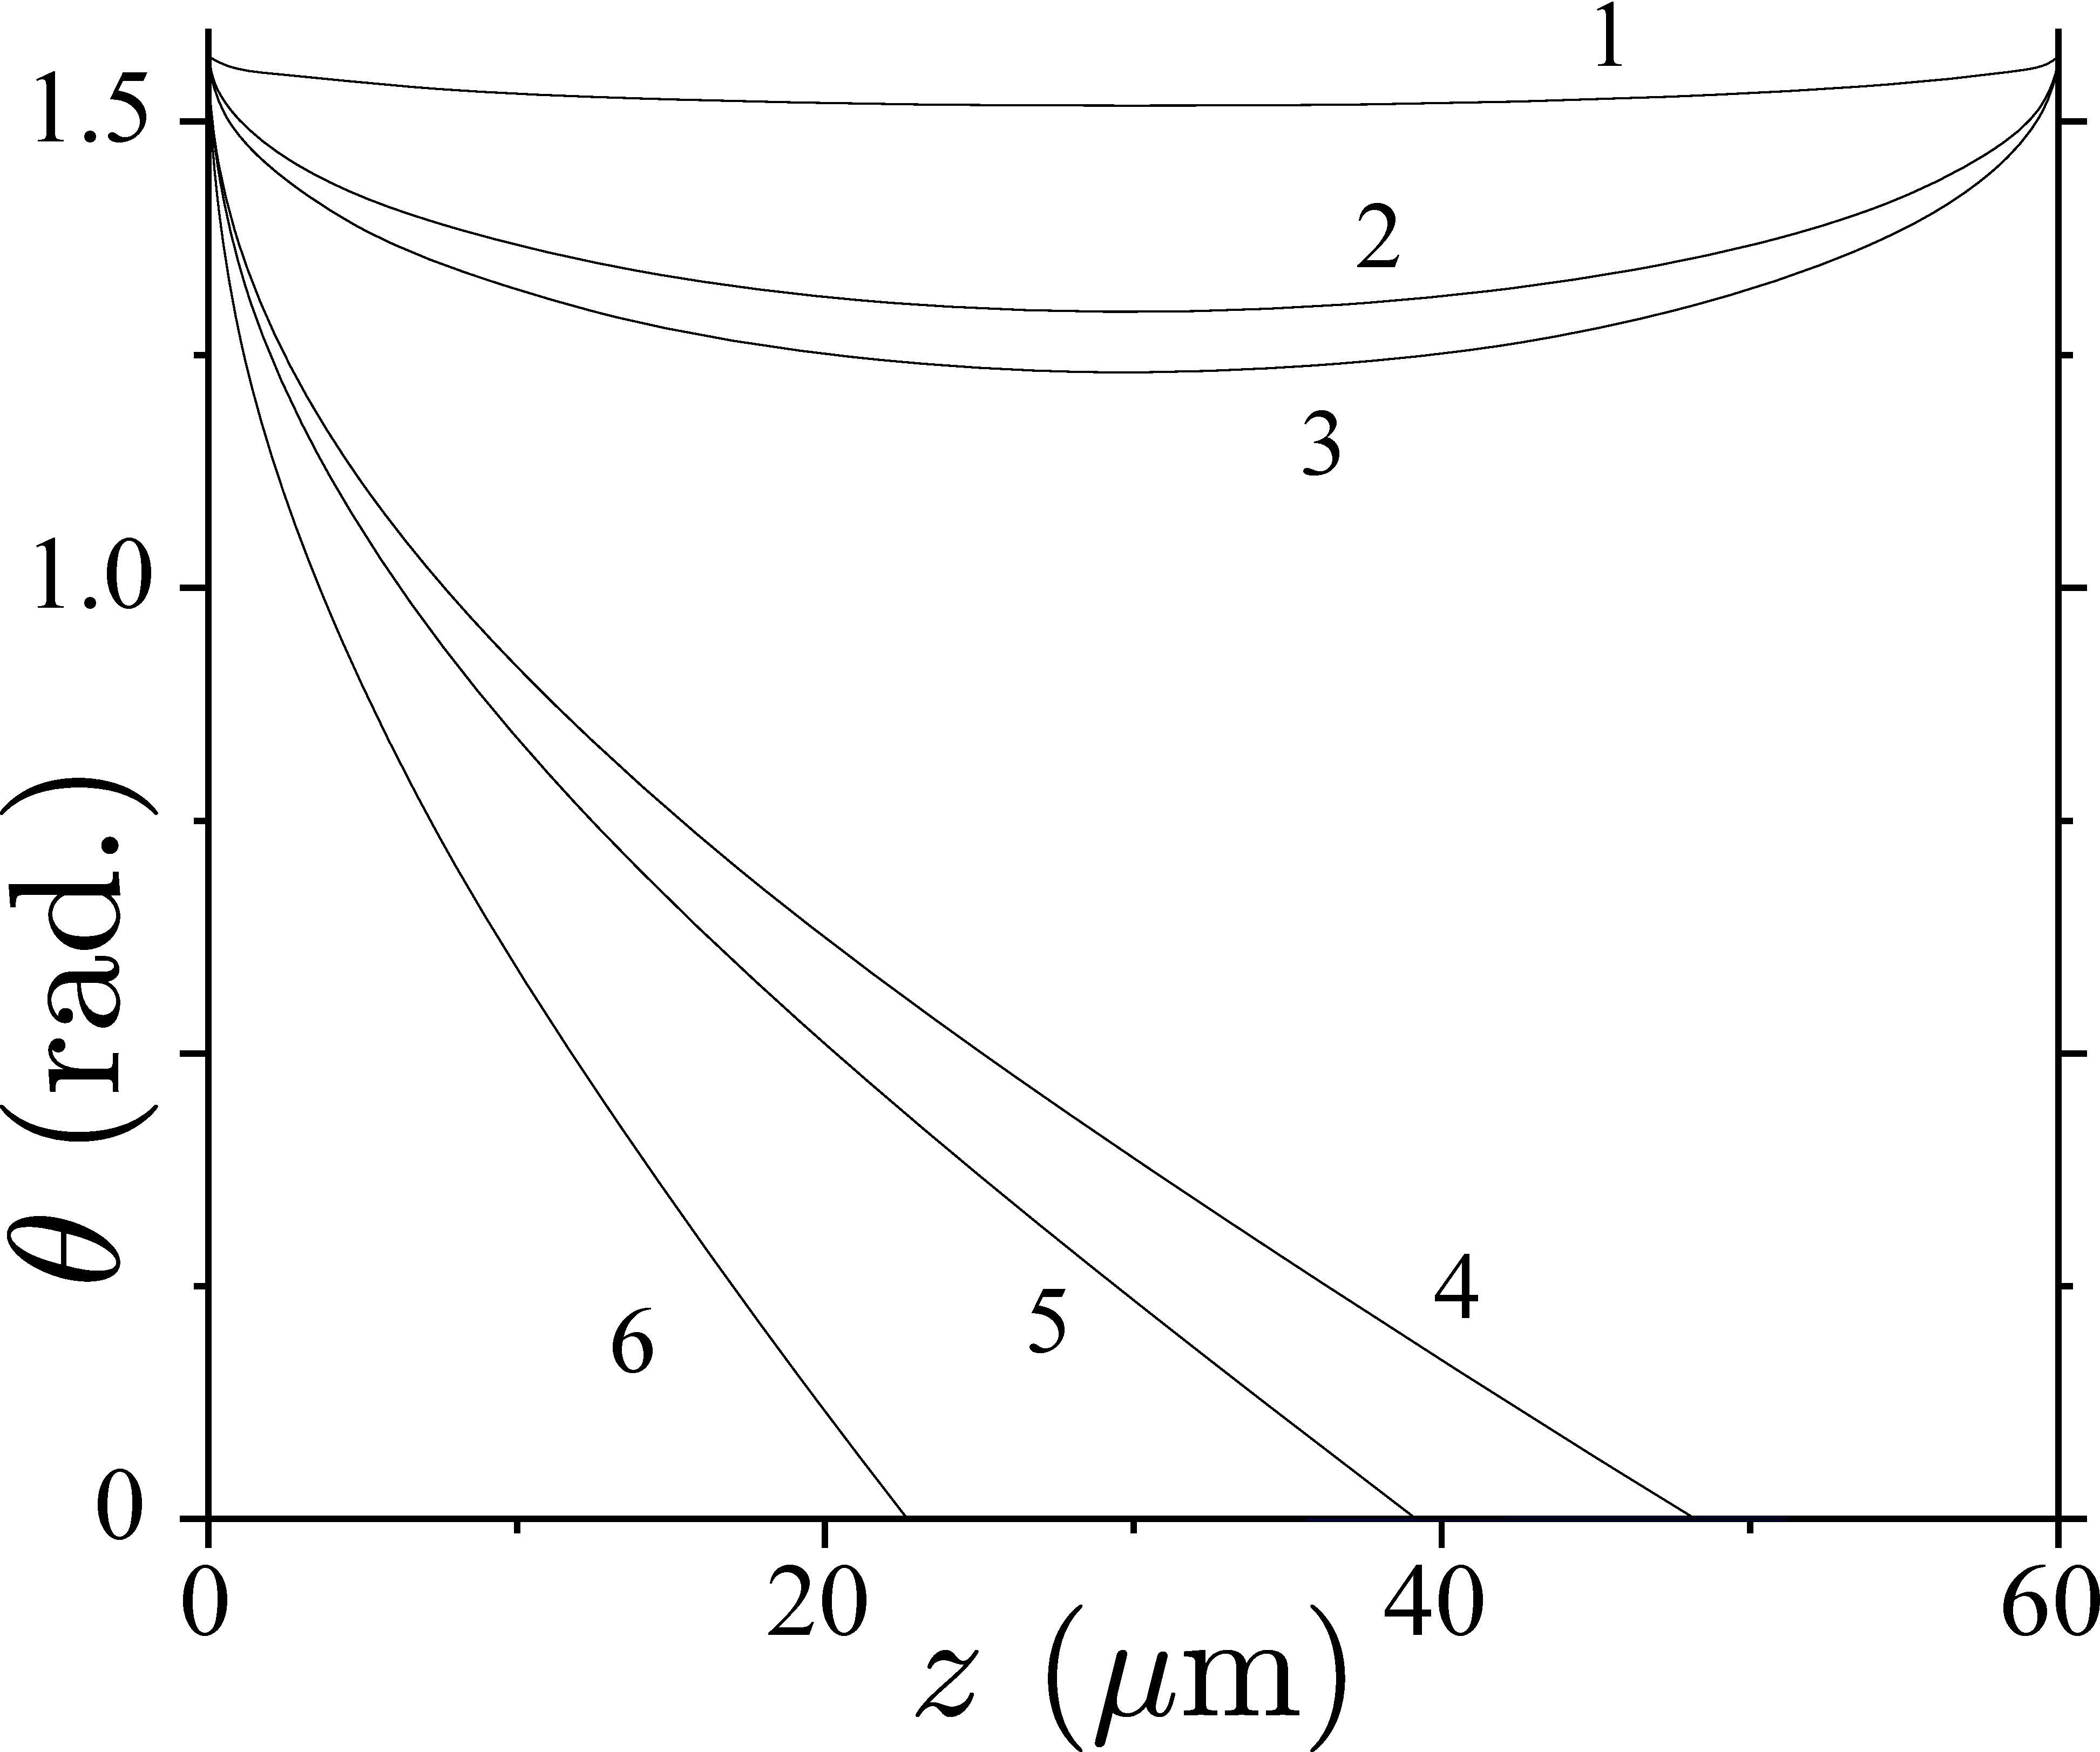
\includegraphics[width=16.9pc]{Fig2_theta_mid_anchoring.eps}\hspace{2pc}%
	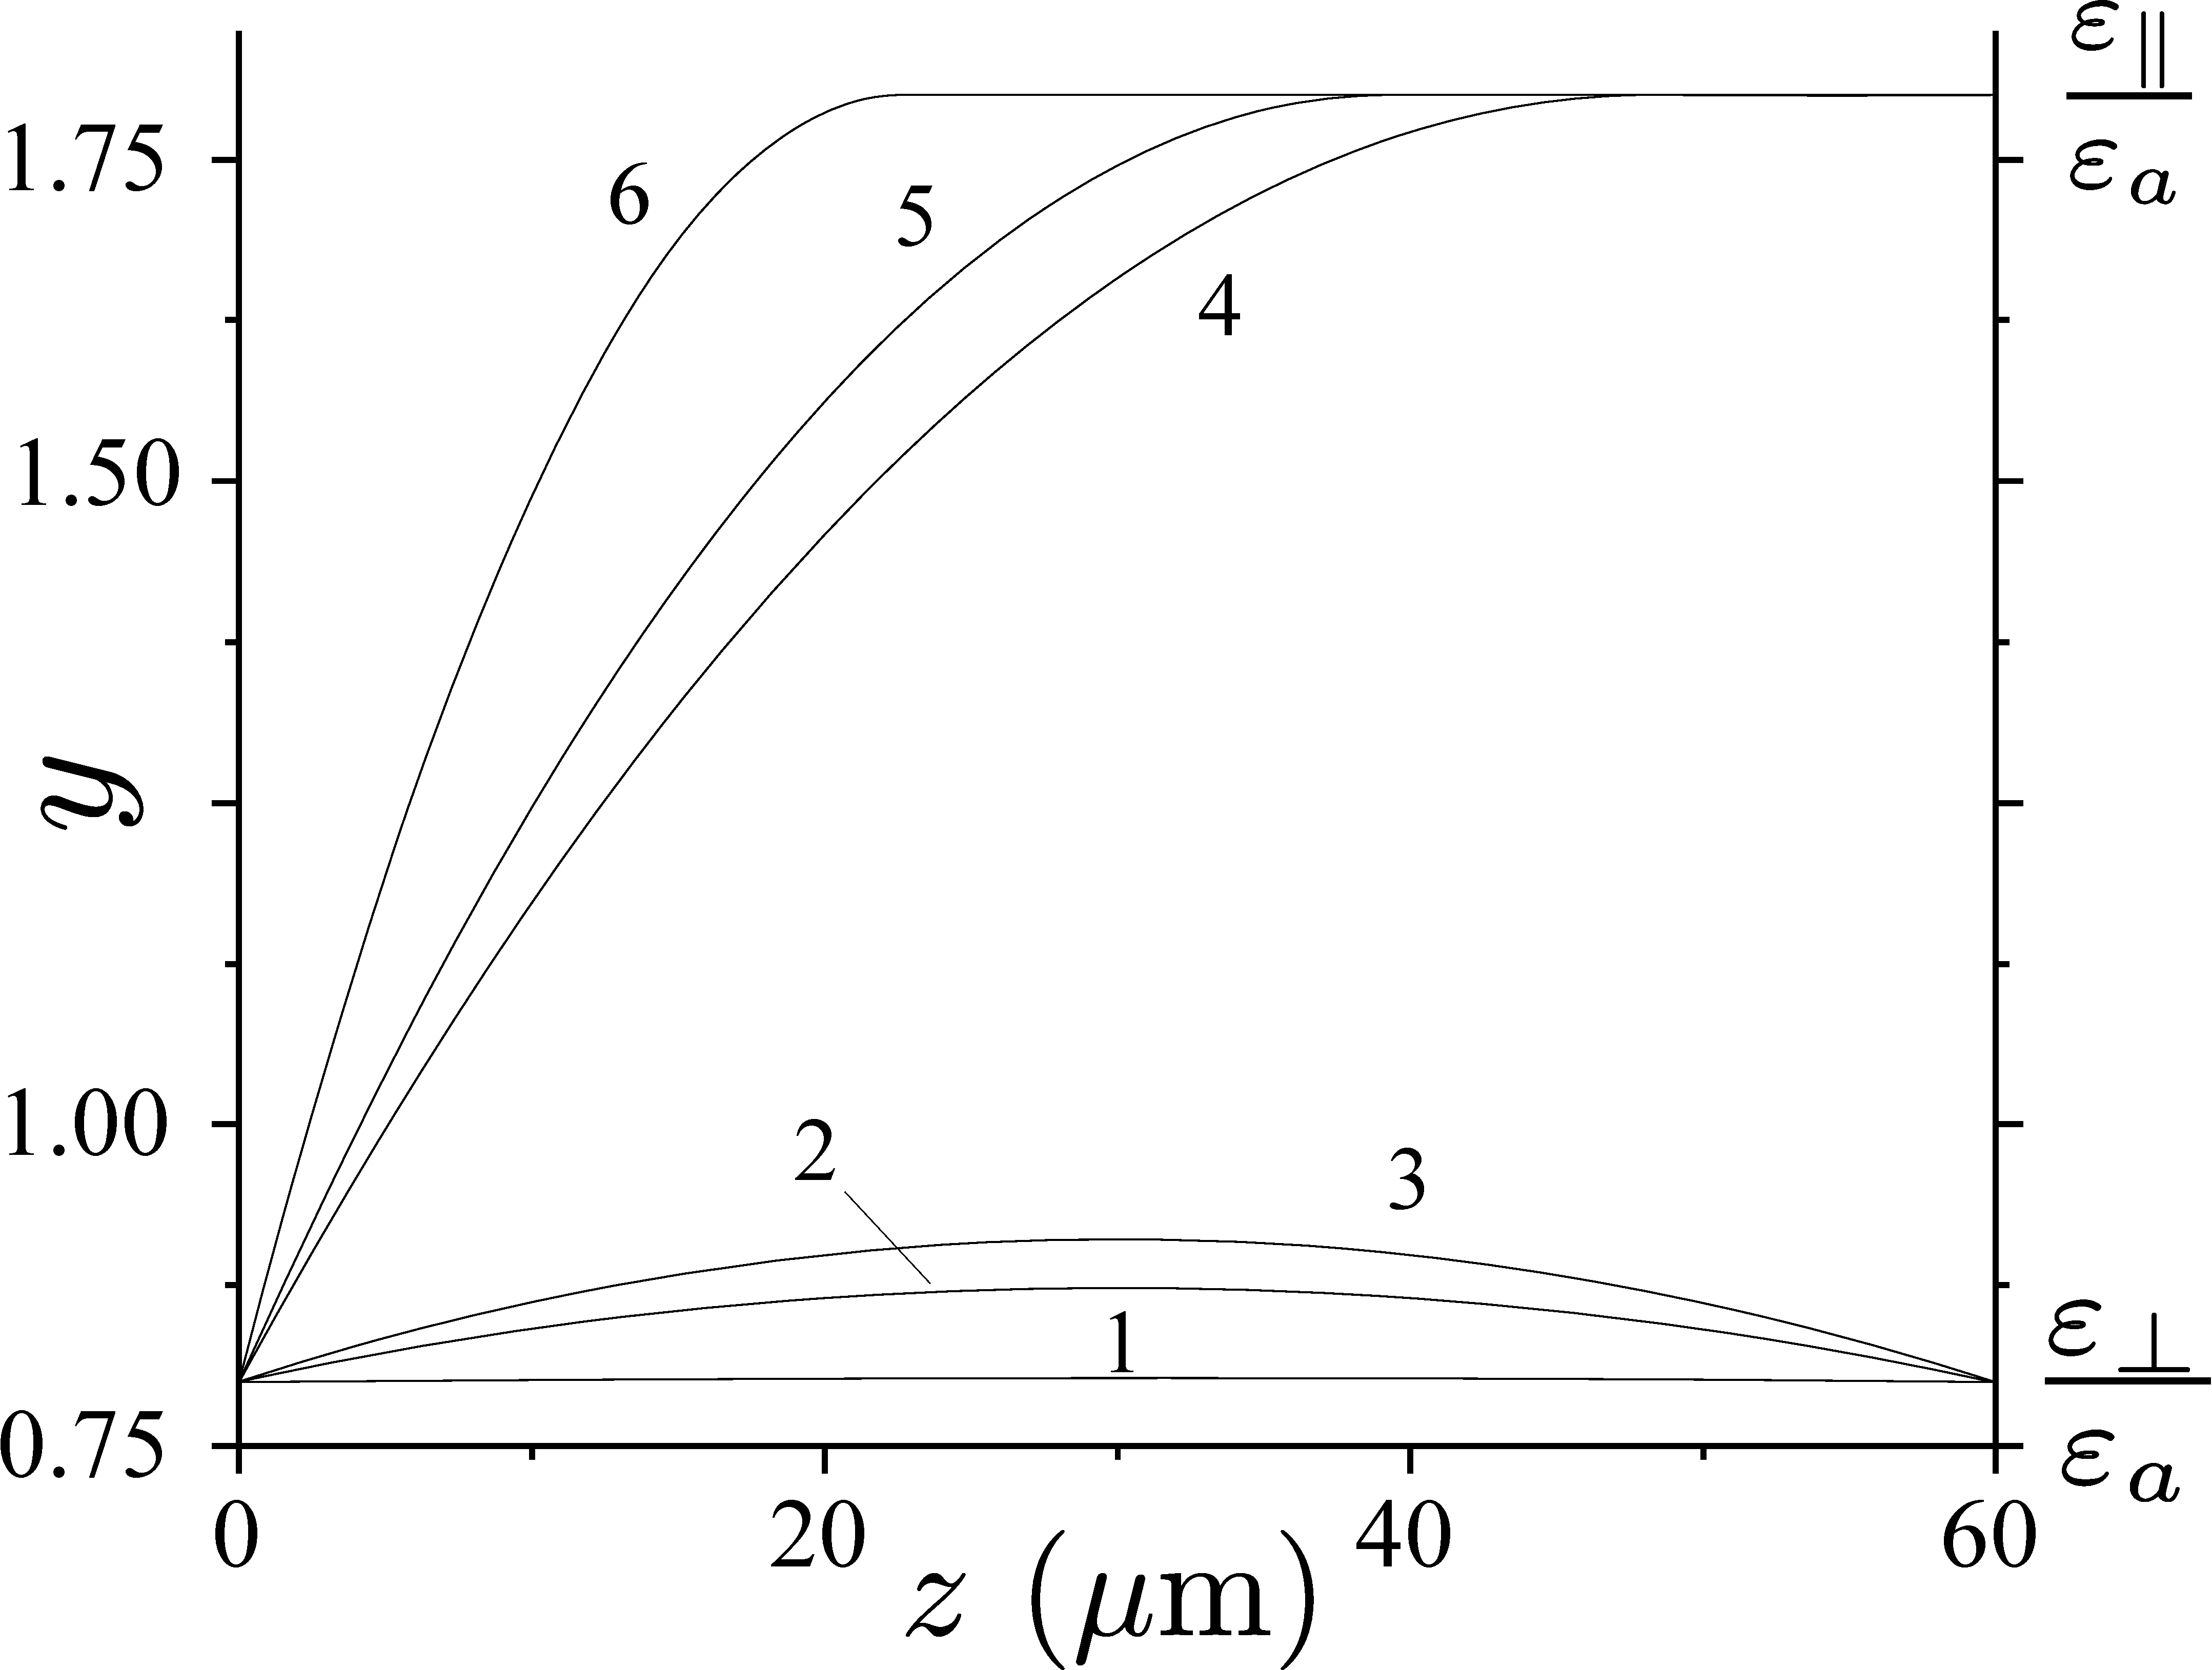
\includegraphics[width=18.9pc]{Fig2_y_mid_anchoring.eps}
	\caption{Графики зависимостей $\theta(z)$ (слева) и $y(z)$ (справа), полученные в случае среднего сцепления с подложкой, когда выполнено неравенство~\eqref{mid_anch}.
		Значения модулей сцепления с подложкой для всех кривых: $W_\theta^{(1)}=0.25\ \text{эрг}/\text{см}^2$, $W_\theta^{(2)} = 0.10\ \text{эрг}/\text{см}^2$.
		Соответствие линий и приложенного напряжения: 1 -- $U = 1$~В, 2 -- $U = 5$~В, 3 -- $U = 6.1$~В, 4 -- $U = 6.2$~В, 5 -- $U = 8$~В, 6 -- $U = 15$~В.}\label{ch5:fig2}
\end{figure}
При этом изменение ориентационной структуры при небольших напряжениях $U$ аналогично происходившим в предыдущем случае, однако когда напряжение достигает значения $\widetilde{U}_1$, происходит скачкообразный переход между кривыми 3 и 4.
Важной особенностью этого случая является то, что область насыщения в объёме ячейки появляется сразу после перехода.
Как и в предыдущем случае, при дальнейшем увеличении напряжения область насыщения в объёме растёт.

\todo{``Сильное зацепление''}

\todo{АО: В описании этого случая ошибка. При отрыве границы она не сразу оказывается насыщенной, и там есть ещё одно характеристическое напряжение}

Наконец, когде энергия сцепления с подложкой удовлетворяет неравенству
\begin{equation}\label{ineq_strong_anch}
g_2L > \frac{4}{\varkappa - 1},
\end{equation}
наблюдается третий сценарий эволюции ориентационной структуры.
\begin{figure}[ht]
	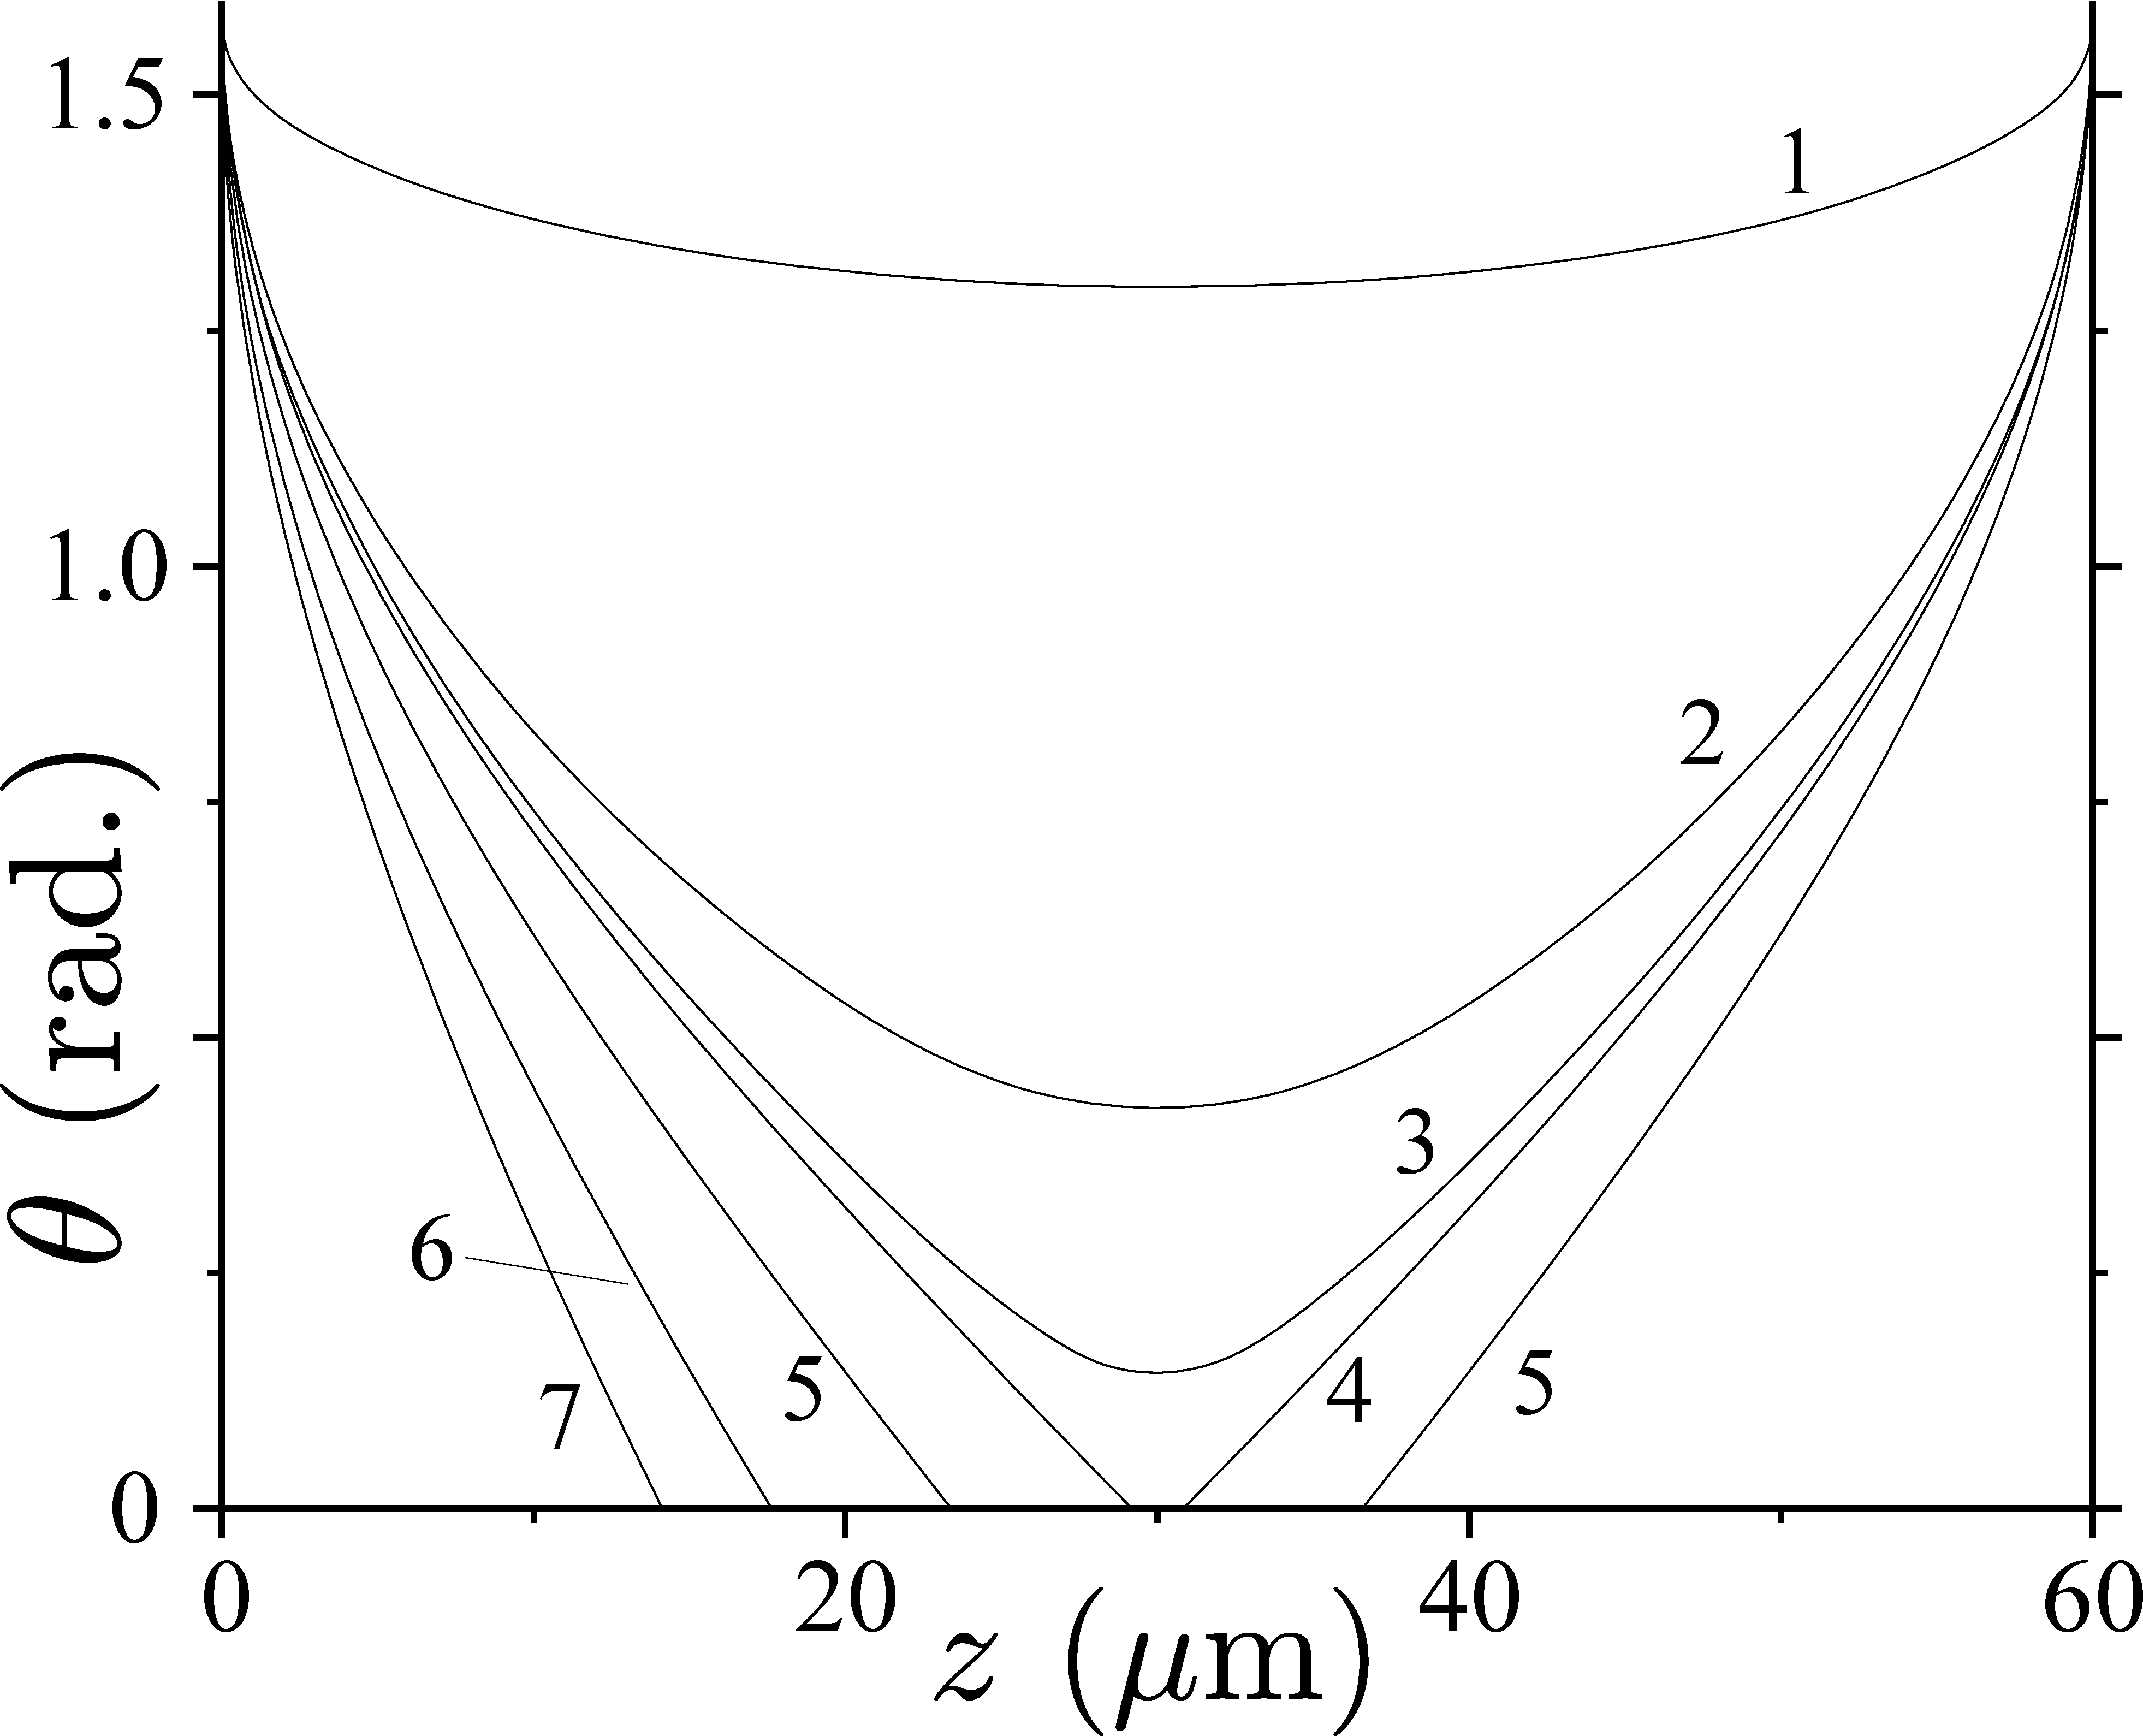
\includegraphics[width=17pc]{Fig3_theta_high_anchoring.eps}\hspace{2pc}%
	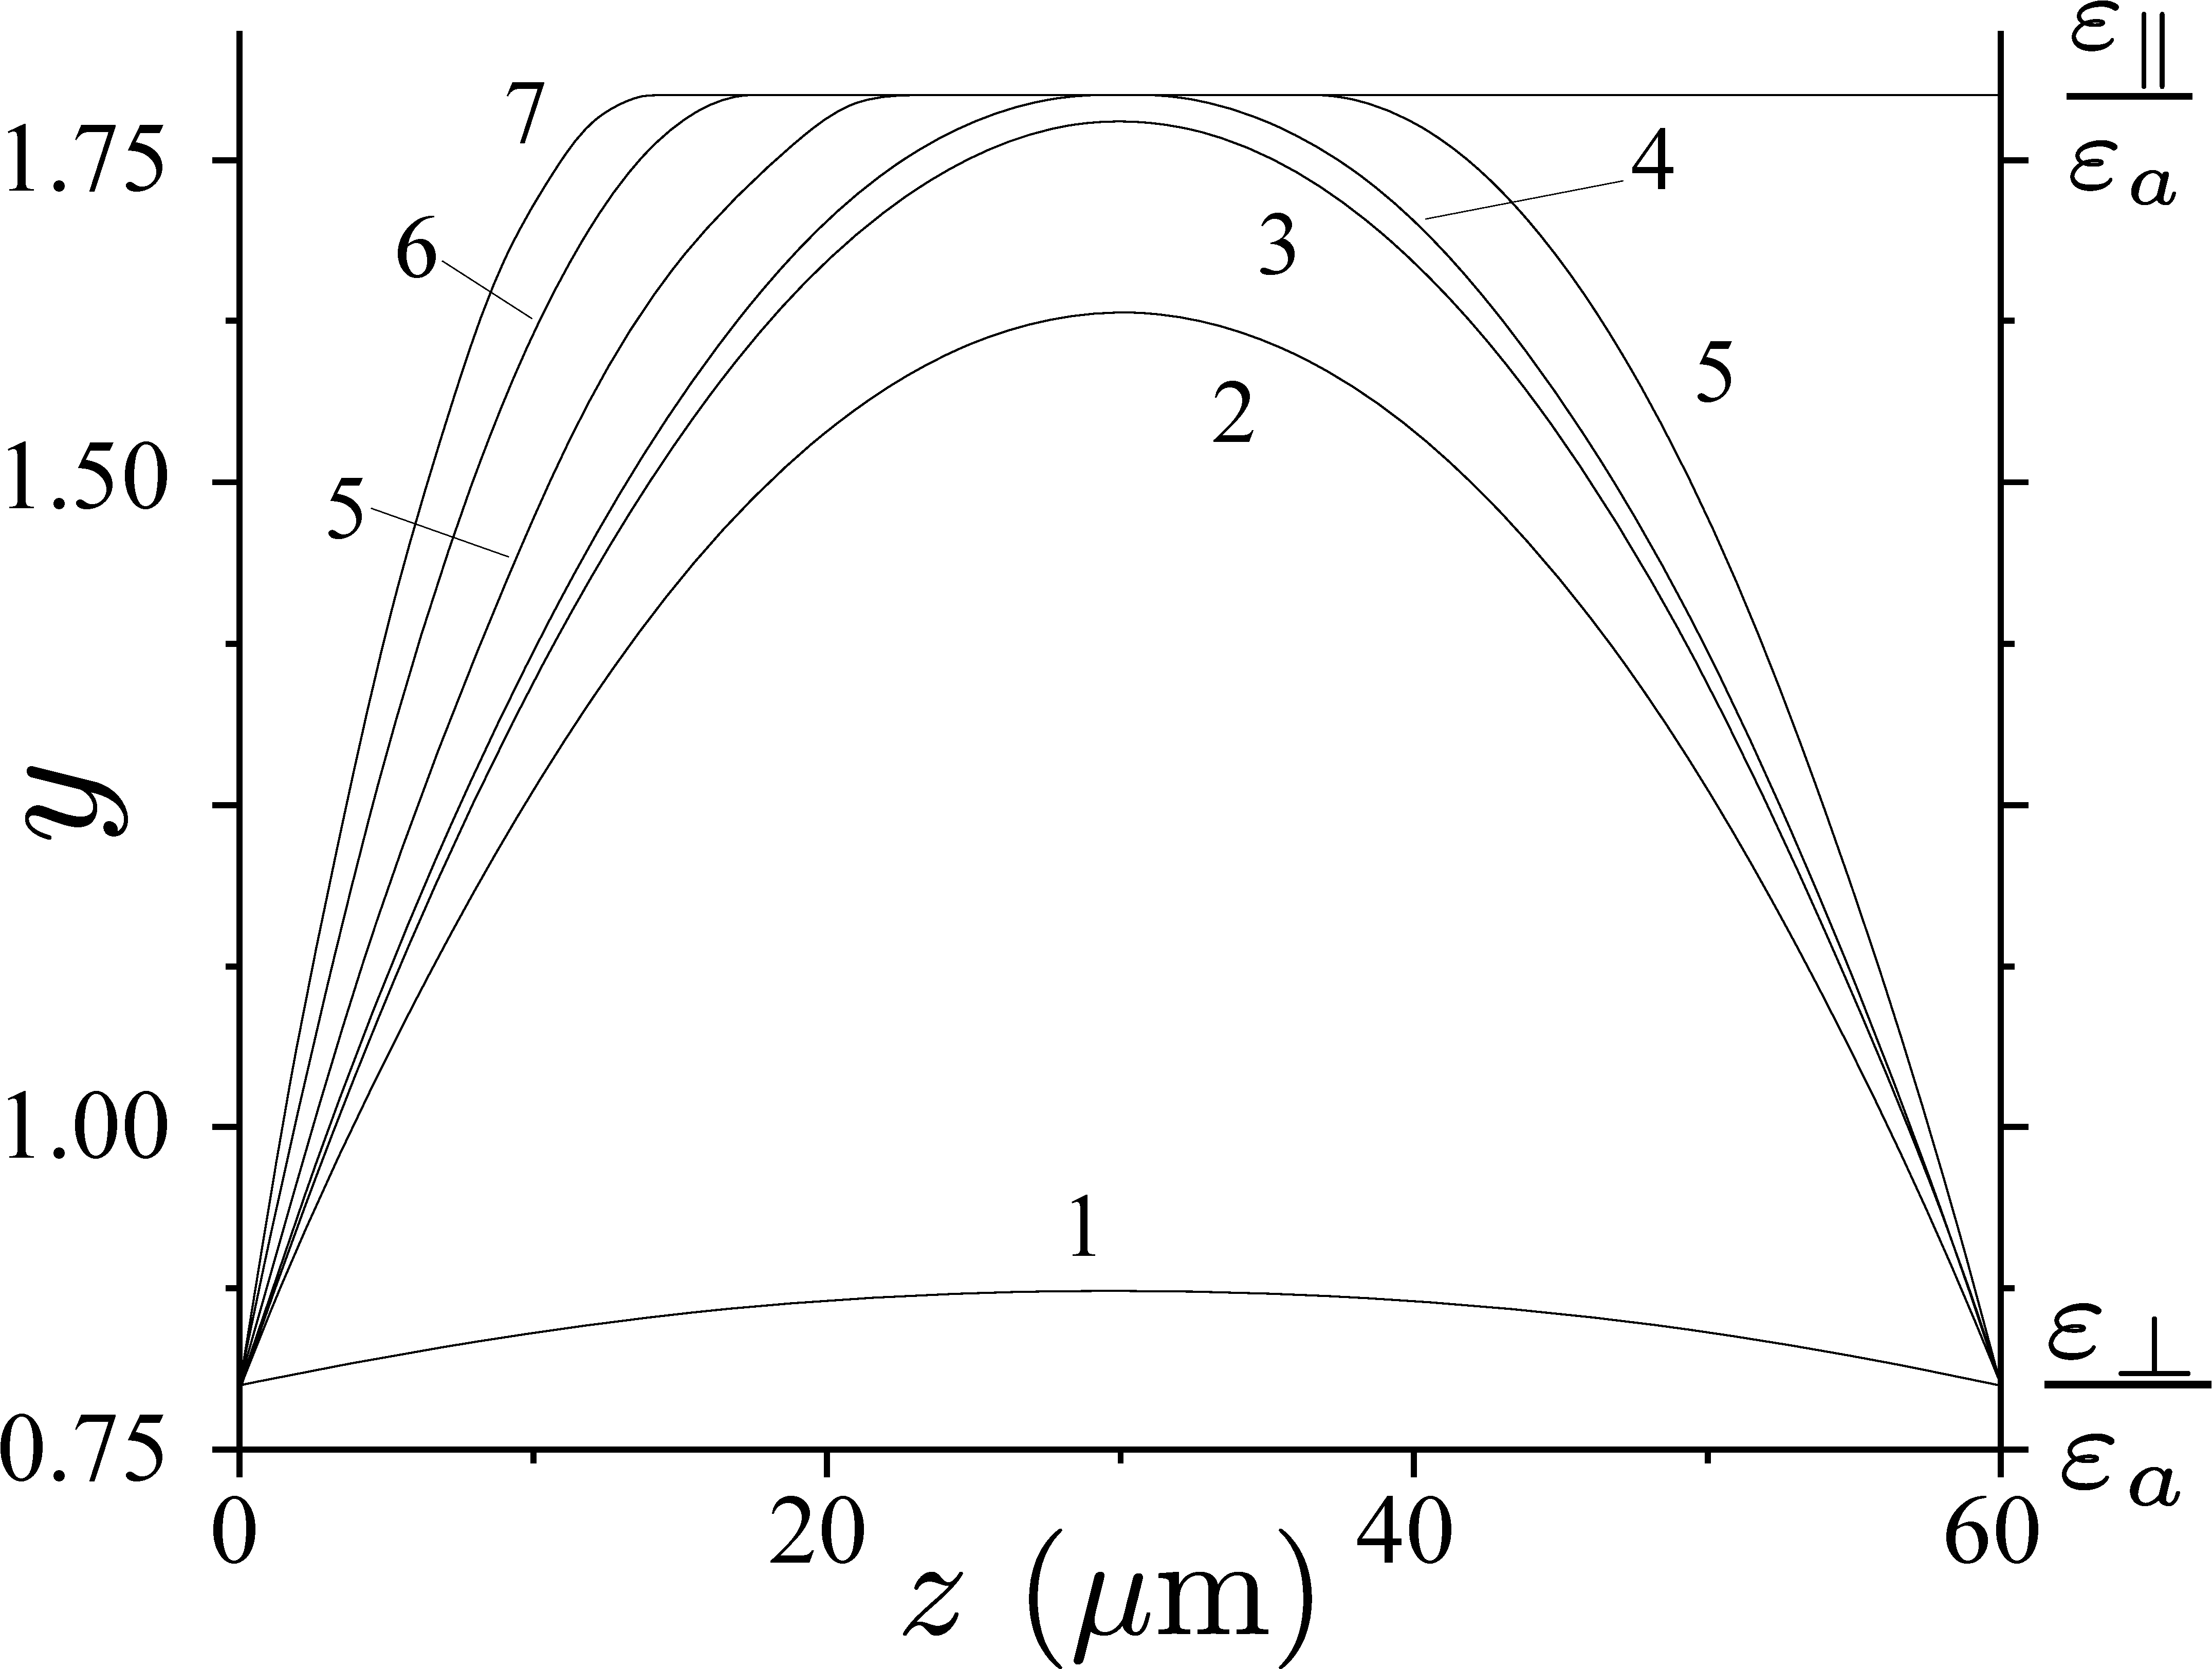
\includegraphics[width=18.9pc]{Fig3_y_high_anchoring.eps}
	\caption{Графики зависимостей $\theta(z)$ (слева) и $y(z)$ (справа), полученные для случая сильного сцепления с подложкой, когда выполнено неравенство~\eqref{ineq_strong_anch}.
		Модули сцепления с подложкой для всех кривых: $W_\theta^{(1)}=1.75\ \text{эрг}/\text{см}^2$, $W_\theta^{(2)} = 0.7\ \text{эрг}/\text{см}^2$.
		Соответствие линий и приложенного напряжения: 1 -- $U = 5$~В, 2 -- $U = 15$~В, 3 -- $U = 16$~В, 4 -- $U = 16.5$~В, 5 -- $U = 19.65$~В, 6 -- $U = 19.75$~В, 7 -- $U = 25$~В.}\label{ch5:fig3}
\end{figure}
Этот сценарий показан на Рис.~\ref{ch5:fig3}.
Опять же, трансформации при малых напряжениях $U$ аналогичны предыдущим случаям.
Однако когда напряжение достигает значения
\begin{equation}
U_2 = \frac{8\pi\bar{e}}{\ve_a}\ln\left( \frac{\varkappa + 1}{\varkappa - 1} \right),
\end{equation} 
в середине ячейки появляется область насыщения (кривые 4 и 5 на Рис.~\ref{ch5:fig3}).
С ростом $U$ эта область продолжает симметрично расширяться от центра ячейки до тех пор, пока напряжение не достигнет значения
\begin{equation}
\widetilde{U}_2 = U_2 + \frac{8\pi \bar{e}}{\ve_a}\left(\frac{g_2L}{2}\cdot\frac{\varkappa}{\varkappa - 1}\cdot \frac{\ve_\bot}{\ve_\parallel} - \frac{2}{\varkappa}\right).
\end{equation}
Когда это происходит, ориентационная структура скачком меняется от описываемой линией 5 на Рис.~\ref{ch5:fig3} до описываемой кривой 6 (при указанном наборе параметров пороговое напряжение составляет $U_2 = 19.68$~В).
Интересно, что если сравнить графики 5 и 6, можно увидеть, что в результате переходе область насыщения расширилась и справа, и слева от центра.
При дальнейшем увеличении $U$ область насыщения также увеличивается (см. линии 6 и 7 на Рис.~\ref{ch5:fig3}).

полученные результаты показывают, что в ячейках с большим усреднённым флексоэлектрическим коэффициентом возможны три сценария эволюции ориентационной структуры с ростом приложенного напряжения.
При этом то, какой сценарий будет реализовываться, зависит от энергии сцепления с одной из границ.
Наши результаты также показали, что в таких ЖК-ячейках возможны разнообразные скачкообразные ориентационные переходы, а также переходы к насыщению.
Такие свойства могут быть использованы при разработке переключателей нового типа.